% -*- root: ../Crypto.tex -*-
\section{Hoja 1}
\begin{problem}[1]
	Un general espartano recibe el siguiente mensaje de un amigo de Cantoblanco:


	SONFAUHPINPEOCTOHRIANEQLSGCUTUOHEEEQOENRUBSETEIDRELEIT

	¿Qué dice el mensaje?

	\solution
	\doneby{Jorge}

	Si consiguiéramos una escítala cuyo diámetro hiciera que entraran 5 letras por fila conseguiríamos el mensaje:

	SUPONGOQUELOHEHECHOBIENPORQUEESDIFICILTENERTANTASUERTE

\end{problem}

\begin{problem}[2]
	Recibes el mensaje VEILRÑW, cifrado usando una clave de Cesar en el alfabeto castellano de 27 letras (con Ñ y W). Lee el mensaje, da las transformaciones para cifrar y descifrar, y cifra el mensaje GRACIAS utilizando la clave correspondiente.

	\solution
	\doneby{Jorge}

	Usando la transformación:
	\[\appl{f_{17}}{ℤ/27}{ℤ/27}\]
	\[f_{17}(x) = x + 17\]

	Se consigue $f_{17}(\{V,E,I,L,R,Ñ,W\}) = \{M,U,Y,B,I,E,N\}$.

	De modo que para cifrar nos basta:
	\[f_{17}^{-1}(x) = f_{-17}(x) = f_{10}(x)\]
	\[f_{10}(\{G,R,A,C,I,A,S\}) = \{P,B,K,M,R,K,C\}\]
\end{problem}

\begin{problem}[3]
	Utilizando el análisis de frecuencias, descifra el siguiente mensaje, del que sabes que está escrito en inglés (26 letras, con W pero sin Ñ) y que ha sido cifrado con una clave de Cesar:
	PXPXKXENVDRUXVTNLXHYMXGMAXYKXJNXGVRFXMAHWGXXWLEHGZXKVBIAXKMXQM

	\solution
	\doneby{Jorge}

	Al hacer el análisis de frecuencias se obtiene:

	\begin{center}
		\begin{tabular}{ l l }
			P & 0.03225806451612903 \\
			X & 0.24193548387096775 \\
			K & 0.06451612903225806 \\
			E & 0.03225806451612903 \\
			N & 0.04838709677419355 \\
			V & 0.06451612903225806 \\
			D & 0.016129032258064516 \\
			R & 0.03225806451612903 \\
			U & 0.016129032258064516 \\
			T & 0.016129032258064516 \\
			L & 0.03225806451612903 \\
			H & 0.04838709677419355 \\
			Y & 0.03225806451612903 \\
			M & 0.08064516129032258 \\
			G & 0.06451612903225806 \\
			A & 0.04838709677419355 \\
			J & 0.016129032258064516 \\
			F & 0.016129032258064516 \\
			W & 0.03225806451612903 \\
			Z & 0.016129032258064516 \\
			B & 0.016129032258064516 \\
			I & 0.016129032258064516 \\
			Q & 0.016129032258064516
		\end{tabular}
	\end{center}

	Se puede ver que la más frecuente entre todas es la letra X. Si tomamos como letra más usada del ingés la E (en vez de la T) se obtiene el mensaje:

	WEWERELUCKYBECAUSEOFTENTHEFREQUENCYMETHODNEEDSLONGERCIPHERTEXT

	Gracias a la transformación $f_{7}(x) = x + 7$.
\end{problem}

\begin{problem}[4]
	La distribución de frecuencias (en porcentaje) en castellano de las 26 letras (es decir, sin W) es aproximadamente la siguiente.

	\begin{tabular}{c c c c c c c c c c c c c c c c c c c c c c c c c c c}
		A & B & C & D & E & F & G & H & I & J & K & L & M \\
		12,6 & 1,0 & 5,1 & 5,7 & 13,7 & 0,9 & 0,8 & 0,5 & 7,0 & 0,2 & 0,0 & 4,6 & 3,2 \\
		N & Ñ & O & P & Q & R & S & T & U & V & X & Y & Z \\
		7,0 & 0,1 & 8,8 & 2,9 & 1,1 & 6,6 & 7,2 & 5,1 & 3,9 & 0,8 & 0,1 & 0,6 & 0,3
	\end{tabular}

	Recibes un mensaje escrito en castellano (con ese alfabeto) que ha sido cifrado con el criptosistema de Cesar. Las dos letras más frecuentes en el texto cifrado son, por ese orden, la J y la N. Deduce razonadamente cual puede haber sido la clave utilizada para cifrar.

	\solution
	\doneby{Jorge}

	Lo lógico sería que las letras más frecuentes en el alfabeto se correspondieran con las más correspondientes en el mensaje, de modo que lo primero que a uno se le viene a la cabeza es corresponder la J (la más frecuente en el mensaje) con la E (la más frecuente en el alfabeto). Esto viene a ser la transformación $f_{-5}=f_{21}$, la cual manda la N (la segunda más frecuente en el mensaje) a la I (que no es la segunda más frecuente en el español).

	De modo que igual la segunda más frecuente en el mensaje es la que se corresponde con la más frecuente en el alfabeto ($f_{-9}=f_{17}$). Con esta transformación se consigue:
	\[f_{17}(J)=A\]
	\[f_{17}(N)=E\]
	Lo cual es más coherente, ya que hace una correspondencia entre las 2 letras más frecuentes del alfabeto (la E y la A) con las 2 más frecuentes del mensaje.
\end{problem}

\begin{problem}[5]
	Interceptamos un mensaje en el que dos profesores hablan de las asignaturas del plan de estudios de Matemáticas. El mensaje es el siguiente:

	DONQONHOSDGXQKCHDKSNSJSDOQOBDCUQ

	Sabemos que el mensaje ha sido cifrado utilizando una sustitución simple en el alfabeto castellano de 27 letras (con Ñ y W), y sospechamos que en el mensaje original aparecía la palabra CALCULO. Lee el mensaje.

	\solution
	\doneby{Jorge}

	Haciendo el análisis de frecuencias del mensaje interceptado se obtiene:

	\begin{center}
		\begin{tabular}{l l}
			D & 0.15625 \\
			O & 0.15625 \\
			N & 0.09375 \\
			Q & 0.125 \\
			H & 0.0625 \\
			S & 0.125 \\
			G & 0.03125 \\
			X & 0.03125 \\
			K & 0.0625 \\
			C & 0.0625 \\
			J & 0.03125 \\
			B & 0.03125 \\
			U & 0.03125
		\end{tabular}
	\end{center}

	Dentro del mensaje interceptado CALCULO se corresponde con NQONHOS, para darse cuenta basta con fijarse que hayan dos pares de letras iguales al igual que pasa en CALCULO. Con dicha correspondencia de letras tenemos (mostramos el mensaje cortado en 2, donde la fila de debajo de cada trozo se corresponde con lo que llevamos descifrado):

	\begin{center}
		\begin{tabular}{c c c c c c c c c c c c c c c c}
			D & O & N & Q & O & N & H & O & S & D & G & X & Q & K & C & H \\
			\_ & L & C & A & L & C & U & L & O & \_ & \_ & \_ & A & \_ & \_ & U
		\end{tabular}
	\end{center}

	\begin{center}
		\begin{tabular}{c c c c c c c c c c c c c c c c}
			D & K & S & N & S & J & S & D & O & Q & O & B & D & C & U & Q \\
			\_ & \_ & O & \_ & O & \_ & O & \_ & L & A & L & \_ & \_ & \_ & \_ & A
		\end{tabular}
	\end{center}

	Puesto que el análisis de frecuencias nos dice que la D es la letra que más aparece, probaremos a corresponderla con la letra E:

	\begin{center}
		\begin{tabular}{c c c c c c c c c c c c c c c c}
			D & O & N & Q & O & N & H & O & S & D & G & X & Q & K & C & H \\
			E & L & C & A & L & C & U & L & O & E & \_ & \_ & A & \_ & \_ & U
		\end{tabular}
	\end{center}

	\begin{center}
		\begin{tabular}{c c c c c c c c c c c c c c c c}
			D & K & S & N & S & J & S & D & O & Q & O & B & D & C & U & Q \\
			E & \_ & O & \_ & O & \_ & O & E & L & A & L & \_ & E & \_ & \_ & A
		\end{tabular}
	\end{center}

	Fijándonos en que la K y la C son las siguientes letras con mayor frecuencia, y que de entre las no utilizadas del alfabeto, la S y N son las siguientes que tienen más frecuencia en español. Probando se llega a que la K va a la N, y la C a la B.

	\begin{center}
		\begin{tabular}{c c c c c c c c c c c c c c c c}
			D & O & N & Q & O & N & H & O & S & D & G & X & Q & K & C & H \\
			E & L & C & A & L & C & U & L & O & E & \_ & \_ & A & N & B & U
		\end{tabular}
	\end{center}

	\begin{center}
		\begin{tabular}{c c c c c c c c c c c c c c c c}
			D & K & S & N & S & J & S & D & O & Q & O & B & D & C & U & Q \\
			E & N & O & \_ & O & \_ & O & E & L & A & L & \_ & E & B & \_ & A
		\end{tabular}
	\end{center}

	Llegados a este punto, somos capaces de adivinar que lo que pone el mensaje es:

	EL CALCULO ES TAN BUENO COMO EL ALGEBRA
\end{problem}


\begin{problem}[6]
	Interceptamos cuatro mensajes cifrados. Sabemos que tanto los mensajes en claro como los mensajes cifrados han sido escritos utilizando el alfabeto inglés de 26 letras. Las frecuencias con que cada letra aparece en cada mensaje son las siguientes:

	\begin{center}
		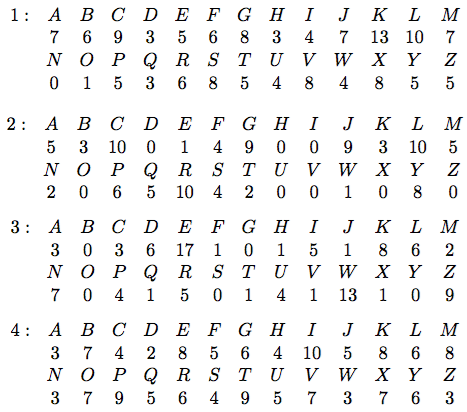
\includegraphics[width=0.5\textwidth]{img/freqsEj1_6}
	\end{center}

	¿Cuáles de los mensajes es razonable pensar que han sido cifrados utilizando sustituciones simples sobre letras?

	\solution
	\doneby{Pedro}

	Lo único que podemos hacer es fijarnos en las frecuencias de las diferentes letras y ver en qué mensajes las letras tienen unas frecuencias similares a las del inglés.

	Basándonos en la tabla de frecuencias de moodle podemos agrupar las letras del alfabeto inglés según la frecuencia con que se usan (en inglés y en cada uno de los mensajes interceptados).

	Si la columna de un mensaje se asemeja a la segunda columna, ese mensaje tendrá alta probabilidad de haber sido cifrado empleando una sustitución simple sobre letras.

	\begin{center}
	\begin{tabular}{| c | c || c | c | c | c |}
	\hline
	\textbf{Porcentaje} & \textbf{Nº Ingles} & \textbf{Nº M1} & \textbf{Nº M2} & \textbf{Nº M3} & \textbf{Nº M4} \\
	\hline
	0-2 & 10 & 2 & 9 & 12 & 0\\
	\hline
	2-4 & 6 & 3 & 4 & 3 & 5 \\
	\hline
	4-6 & 1 & 8 & 5 & 3 & 7 \\
	\hline
	6-8 & 7 & 6 & 1 & 3 & 8 \\
	\hline
	8-10 & 1 & 5 & 3 & 2 & 5 \\
	\hline
	>10 & 1 & 2 & 3 & 2 & 1 \\
	\hline
	\end{tabular}
	\end{center}

	Antes de nada hay que comentar que no sabemos qué longitud tenía cada mensaje por lo que tampoco sabemos cómo de válidas son las frecuencias calculadas. Por ello se ha tomado la decisión de agrupar las frecuencias por valores.

	Si sabemos que cada mensaje era un ``Los Pilares de la Tierra'' en inglés y cifrado, tendremos unas estimaciones de la frecuencia de cada letra muy muy buenas, por lo que podríamos agrupar las frecuencias por unidades.

	El primer y el último mensajes tienen muy pocas letras con baja frecuencia y demasiadas con frecuencia 8-10 por lo que parece razonable descartar la posibilidad de que hayan sido escritos en inglés.

	Entre el segundo y el tercero, el que más posibilidades tiene de haber sido escrito originalmente en inglés es el tercero, pues el segundo tiene muy pocas letras con frecuencia 6-8 y quizás demasiadas con frecuencias altas.

	Para el espía experto otra posibilidad sería estudiar la media y la varianza de la distribución de frecuencias en cada mensaje y apoyarse también en eso a la hora de tomar la decisión.
\end{problem}


\begin{problem}[7]
	En un alfabeto de 28 letras, las 27 del castellano y el espacio=27, utiliza la clave afíın sobre letras $f(m) = 13m + 9$ para cifrar el mensaje ``MUY BIEN''.

	\solution

	\doneby{Jorge}

	Utilizamos el $\_$ para representar el espacio y que este se vea claro.
	\[f(``MUY\_BIEN'')=``SXTRPW\_E''\]
\end{problem}


\begin{problem}[8]
	Sabemos que el enemigo está utilizando transformaciones afines sobre letras para cifrar mensajes escritos en inglés con el siguiente alfabeto de 37 letras: los números 0,...,9 que se codifican como ellos mismos; las letras A,…,Z (con W, sin Ñ), que corresponden a 10,…,35; y el espacio en blanco=36. Interceptamos el siguiente mensaje cifrado

	OH7F86BB46R3627O266BB9 (Atención, no hay ceros, sólo os)

	Sabiendo que el mensaje original acaba con la firma 007 (cero, cero, siete), ¿qué dice el mensaje?

	\solution
	\doneby{Jorge}

	La transformación afín será de la forma:
	\[ f_{a,b}(x) = ax+b \]

	Luego planteando un sistema de ecuaciones obtenemos a y b, sabemos que B=11:
	\[ f_{a,b}(11) = a·11 + b = 0\]
	\[ f_{a,b}(9)  = a·9  + b = 7 \]

	\[ b = -11a = 26a \]

	Luego
	\[ 9a + 26a = 35a = 7 \implies a = 15  \implies b = 20\]

	Aplicando $f_{a,b}$ al mensaje cifrado se obtiene:
	\begin{center}
		``AGENT 006 IS DEAD  007''
	\end{center}
\end{problem}


\begin{problem}[9]
	Una unidad de texto (en claro) m se dice que es fija para una transformación para cifrar si $f(m) = m$. Supongamos que estamos usando transformaciones afines sobre letras en un alfabeto de N letras, $f(m) = a · m + b$ con $a ≠ 1$.

	\begin{enumerate}
		\item Demostrar que si N es primo hay exactamente una letra fija.
		\item Demostrar que para N arbitrario cualquier transformación lineal (es decir, con b = 0) tiene al menos una letra fija, y que si N es par cualquier transformación lineal tiene al menos dos letras fijas.
		\item Dar un ejemplo de una transformación afín (para algún N) sin letras fijas.
	\end{enumerate}

	\solution
	\doneby{Jorge}
	\begin{enumerate}
		\item $m = a · m + b  \implies (a-1)·m + b = 0 \implies m = -(a-1)^{-1} · b$. En caso de que $N$ sea primo sabemos que existe $(a-1)^{-1}$, ya que en ese caso $U(ℤ/N)=ℤ/N$ y por tanto $(a-1) ∈ U(ℤ/N)$. Así que $m$ es único al quedar determinado por el producto de $(a-1)^{-1}$ y $b$.

		\item En caso de que $f(m) = a·m$ sabemos que siempre tendremos la letra fija asociada al 0 (ya que $f(0)=0$) independientemente de qué $N$ tengamos.

		Si $f(m) = a·m$ con $N$ par ($N=2M$), se cumple, además, que $f(M)=M$, ya que

		\[f(M)=M \iff aM = M \iff (a-1)M = 0 \iff 2M | (a-1)M \]

		Y puesto que $a$ debe ser unidad en $\ent_{2M}$, debe ser coprimo con $2M$ y, por tanto, impar. Por tanto, es claro que $(a-1)$ será par y, efectivamente $(a-1)M = k \cdot 2M$

		\item Para $N=2$ la transformación $f(x) = x + 1$ no deja letras fijas.
	\end{enumerate}
\end{problem}

\begin{problem}[10]
	Sea $A$ un anillo conmutativo con 1. Diremos que $a∈A$ es un divisor de 0 si existe $b∈A$, $b≠0$ y tal que $ab = 0$ (con esta definición, que no es la normal, 0 es un divisor de 0, pero no importa, simplifica los enunciados). Diremos que $a ∈ A$ es una unidad si existe $b ∈ A$ tal que $ab = 1$.

	\ppart Demostrar que $\left\{ \text{Unidades de } A \right\} ∩ \left\{ \text{Divisores de 0 en } A \right\} = \emptyset$
	\ppart Dado $a ∈ A$, definimos la aplicación ``multiplicar por $a$'', $\appl{m_a}{A}{A}$ como $m_a(x) = ax$. Caracterizar los divisores de 0 (o quizá los no divisores de 0) y las unidades de $A$ en términos de propiedades de la correspondiente aplicación $m_a$.
	\ppart Utilizar la caracterización anterior para demostrar que si $A$ es un anillo finito se tiene:

		\[\left\{ \text{Unidades de } A \right\} \cup \left\{ \text{Divisidores de 0 en } A \right\} = A\]

		(Esto generaliza lo que sucede en los anillos de congruencias $ℤ/Nℤ$.)
	\ppart Demostrar que la hipótesis de finitud es esencial en el apartado 3.

	\solution
	\doneby{Pedro}

	\spart
	Supongamos que tenemos un elemento $x$ que es unidad y divisor de 0 simultáneamente.

	En ese caso tendríamos que existen dos números $a$ y $b$, ambos distintos de 0, tales que: $ax = 0$ y $bx = 1$

	En esta situación podemos tomar la ecuación $bx=1$ y multiplicar por $a$ a ambos lados, con lo que mantenemos la igualdad, obteniendo:
	\[bx = 1 \iff abx = a \iff axb = a \iff 0 \cdot b = a \iff 0 = a\]

	Con lo que llegamos a una contradicción, pues dijimos que $a \neq 0$

	\spart

	Si tenemos que $a$ es un divisor de 0, habrá algún valor (distinto de 0) que nos llevará a 0, con lo que la función $f_a$ no será inyectiva.

	A raíz de esto podemos ver que si $a$ no es un divisor de 0, la función $m_a(x)=ax$ será inyectiva. Para comprobarlo basta con ver que:
	\[\forall x\neq y, \ ax=ay \implies a(x-y)=0 \implies a \text{ divisor de 0 ya que } x-y \neq 0\]
	lo que nos lleva a una contradicción.

	Por otro lado, si $a$ es una unidad, la función será sobreyectiva pues tendremos:
	\[\forall y \ ax = y \implies x = ya^{-1} \implies \exists x \tq m_a(x)=y\]

	Además, de esta misma fórmula podemos deducir que si no es unidad, no será sobreyectiva la función (no podremos llegar al 1, por ejemplo)

	\spart

	Si tenemos un elemento $a \in A$ que no es unidad ni divisor de 0 en $A$, tendremos que la función asociada $m_a$ será inyectiva pero no sobreyectiva.

	Si una función entre dos conjuntos finitos es inyectiva pero no sobreyectiva, esto implica que el conjunto de partida es menor que el de llegada. Pero por definición, la función $m_a$ va de un conjunto en si mismo, con lo que es imposible que sea inyectiva y no sobreyectiva.

	Por tanto es imposible que exista un $a$ como el que hemos definido. Es decir, tenemos demostrado que
	\[\left\{ \text{Unidades de } A \right\} \cup \left\{ \text{Divisidores de 0 en } A \right\} \supset A\]

	El otro sentido del contenido es trivial por la propia construcción del conjunto de unidades y de los divisores.

	\spart

	Si $A$ se tratase del anillo $(\ent, +, \cdot )$, dado $a=2$ podemos construir una aplicación $m_a$ que, como se probó en el apartado anterior, sería inyectiva pues 2 no es divisor de 0.

	Sin embargo, al no ser un cuerpo finito no hay problema en que una función vaya de un anillo en si mismo siendo inyectiva pero no sobreyectiva. Por tanto no podríamos deducir ninguna relación de contención.

	\doneby{Edu}

	\spart[a]

	Supongamos x $\in \text{Unidades de } A$ y $\exists y \neq 0 \tq x\cdot y = 0$, ie, x $\in \text{Divisores de 0 en } A$:
	\[ x \cdot y = 0 \implies x^{-1} \cdot x \cdot y = 0 \implies y = 0 \Rightarrow \Leftarrow \]
	{\bf Conclusión:} si x $\in \text{Unidades de } A \implies$ x $\not\in \text{Divisores de 0 en } A$

	Supongamos x $\in \text{Divisores de 0 en } A$, ie, $\exists y \neq 0 \tq x \cdot y = 0$ y supongamos $\exists z \neq 0 \tq x \cdot z = 1$:
	\[ x \cdot z = 1 \implies y \cdot x \cdot z = y \cdot 1 \implies 0 \cdot z = y \implies 0 = y \Rightarrow \Leftarrow \]
	{\bf Conclusión:} si x $\in \text{Divisores de 0 en } A  \implies$ x $\not\in \text{Unidades de } A$
	\newline\qed

	\spart[b]

	Si $m_a$ es inyectiva (y {\bf por ser A finito} entonces es sobreyectiva)

	$\implies \forall x,y \neq 0 \in A$, $m_a(x) = xa = ya = m_a(y) \implies x = y \implies $ a $\in $ unidades de A ya que, al ser {\bf sobreyectiva}, $\exists y \in A \tq a\cdot y = 1$.

	Si $m_a$ no es sobreyectiva, ie, GCD($m\cdot a$, |A|) $> 1$ para algún a, $\exists x,y \in A, x \neq y \tq$ $a \cdot x = a \cdot y \implies a (x - y) = 0 \implies a$ es divisor de 0.

	\spart[c]

	Como observación, diremos que si la afirmación es falsa, por el apartado 1, tiene que existir un $x$ que no pertenece a ninguno de los dos subconjuntos de A, lo cual es imposible por el apartado anterior: si $m_a$ es inyectiva, entonces $a$ es unidad, si $m_a$ no es sobreyectiva, $a$ es divisor de 0.
\newline\qed

	\spart[d]

	Leer la parte negrita del apartado B y convencerse de que no tiene por qué existir el inverso de $a$.

\end{problem}





\section{Control 1 (22-09-2014) Modelo A}
\begin{problem}[1]
Dado $N\geq 2$ y un elemento $a \in \ent_N$, consideramos la aplicación $\appl{m_a}{\ent_N}{\ent_N}$ tal que $m(x)=ax$.

Demostrar que son equivalentes:
\begin{enumerate}
\item $a$ es unidad en $\ent_N$
\item $a$ y $N$ son primos entre si.
\item $m_a$ es inyectiva
\item $m_a$ es sobreyectiva
\end{enumerate}

\solution
\doneby{Pedro}

Para demostrar que los enunciados son equivalentes vamos a demostrar una serie de implicaciones de modo que, al final, desde cualquiera de esas afirmaciones podamos llegar a cuaquier otra.

\begin{itemize}
\item \textbf{$1 \implies 2$}
Si $a$ es una unidad en $\ent_N$ sabemos que existe $c \in \ent_N$ tal que
\[ac = kN + 1\]

Supongamos ahora que $a$ y $N$ no son primos entre si, es decir,
\[\exists b \tq a = b \cdot a' \text{ y } N = b \cdot N'\]

Sustituyendo en la primera fórmula obtenemos
\[ba'c=bkN'+1 \iff b(a'c-kN')=1 \iff b \in U(\ent_N)\]

Pero está claro que $b$ no puede pertenecer a las unidades de $\ent_N$ ya que, siempre que $bc< N$ es claro que $bc \neq 1$ salvo que ambos sean 1 y, además:
\[\forall c \in \ent_N, \tq cb > N \iff cb = bN'α+bβ \text{ siendo } bβ < N\]
con lo que el resto nunca será 1.

\item \textbf{$2 \implies 3$}

Ahora tenemos $a$, $N$ tales que $(a,N)=1$ y queremos ver que la función $m_a$ es inyectiva.

Suponemos que no es inyectiva y que por tanto $\exists x,y \in \ent_N$ tales que $x \neq y$ y:
\[ax=ay \text{ mod } n \iff a(x-y)= 0 \ \text{mod } n \iff a(x-y) = c N\]

Pero, en caso de ser esto cierto, por definición, $a$ sería un divisor de $cN$ y, por tanto, $a$ divide a $c$ ya que estamos considerando $(a,N)=1$.

Si $a$ fuese divisor de $c$, podríamos escribir:
\[a(x-y)=kaN \iff (x-y) = kN\]
pero consideramos que $x$ y $y$ son dos elementos distintos de $\ent_N$ y, por tanto, su diferencia no puede ser múltiplo de $N$. Con lo que llegamos a una contradicción.

Por tanto no pueden existir $x$, $y$ como los descritos con lo que queda claro que la función es inyectiva.

\item \textbf{$3 \implies 4$}
Como estamos moviéndonos en un conjunto finito, si la función es inyectiva debe ser también sobreyectiva.

\item \textbf{$4 \implies 1$}

Si la función es sobreyectiva, entonces
\[\forall c \in \ent_N \exists b \in \ent_N \tq ab=c\]
en concreto esto es cierto para $c=1$ y por tanto $a$ tiene inverso, es decir, pertenece a las unidades de $\ent_N$

\end{itemize}

\end{problem}

\begin{problem}[2]
En un idioma que se escribe usando el mismo alfabeto que el inglés (26 letras), las letras más frecuentes son $B(20\%)$ y $Z(13\%)$, sin que ninguna de las demás letras tenga una frecuencia superior al $5\%$

Interceptamos un texto escrito en este idioma que ha sido cifrado usando un criptosistema afín sobre las letras vistas como elementos de $\ent_{26}$. Las letras más frecuentes en el mensaje cifrado resultan ser, por este orden, $H$ y $D$.

¿Qué letra en claro dirías que corresponde con la $E$ cifrada?

\solution
\doneby{Pedro}

Vamos a calcular directamente la función de descifrado, que será de la forma $f(m)=αm+β$. Sustituyendo los datos que tenemos nos queda el sistema:
\[\left\{
7α +β  = 1 \atop
3α + β = 25
\right. \implies 22α = 24 \implies 11α = 12 \]

Para resolver la ecuación tenemos que calcular el inverso de $11$ módulo 26. Para ello aplicamos el algoritmo de Euclides:
\[\begin{array}{l}
26 = 2 \cdot 11 +4\\
11 = 2 \cdot 4+ 3\\
4 = 1 \cdot 3 + 1
\end{array} \implies \begin{array}{l}
1 = 4 - 3 \\
3 = 11 - 2 \cdot 4 \implies 1 = 4 - 11 + 2 \cdot 4 = 3\cdot 4 -11 \\
4 = 26 -2 \cdot 11 \implies 1 = 3 \cdot 26 -6\cdot 11 - 11 = 3 \cdot 26 -7\cdot 11
\end{array}\]

Finalmente tenemos que $1 = 3\cdot 26 + 19 \cdot 11$, con lo que podemos resolver la ecuación, pues
\[α = 19 \cdot 12 = 20 \implies β = 17\]

Ahora podemos descifrar la letra $E$ obteniendo:
\[f(E)=f(4) = 15 = P\]
\end{problem}


\section{Hoja 2}
\begin{problem}[1]
El enemigo escribe en inglés y, para cifrar sus mensajes, utiliza transformaciones afines sobre digrafos en el siguiente alfabeto de 30 letras: las letras A,...,Z (con W, sin Ñ) corresponden a 0,...,25; el espacio=26; ?=27; !=28; ’=29. Interceptamos el siguiente mensaje cifrado:
\begin{center}
DXM SCE DCCUVGX
\end{center}

Un análisis de frecuencias sobre texto interceptado con anterioridad muestra que los digrafos más frecuentes son, por este orden, “M ”, “U ” e “IH”.

En inglés escrito con este alfabeto los digrafos más frecuentes son, por orden, “E ”, “S ” y “ T”.
\ppart Encuentra la clave para descifrar y lee el mensaje.
\ppart Encuentra la clave para cifrar y encripta el mensaje YES I’M JOKING!

\solution

\doneby{Pedro}

\spart
La función que emplearemos para descifrar el mensaje será de la forma: $f(m)=αm+β$ siendo α una matriz 2x2.

Así podemos plantear el sistema de ecuaciones:
\[
\left\{
386α+β = 146 \atop
626α+β = 566
\right. \implies 240α = 420\]

Ahora debemos calcular el inverso de 240 módulo $30 ^2 = 900$ pero 240 no es coprimo con 900 por lo que no será invertible.

Vamos a emplear el tercer par de letras más frecuentes para intentar plantear un sistema que podamos resolver. Así llegamos a
\[
\left\{
386α+β = 146 \atop
247α +β = 799
\right. \implies 761α = 653\]

Empleamos ahora el algoritmo de euclides para calcular el inverso de 761 en $\ent_{900}$
\[\begin{array}{l}
900 = 761 + 139\\
761 = 5\cdot 139 + 66 \\
139 = 2 \cdot 66 + 7\\
66 = 9\cdot 7 + 3 \\
7 = 2 \cdot 3 + 1
\end{array} \implies \begin{array}{l}
1 = 7 - 2 \cdot 3 \\
3 = 66 - 9 \cdot 7 \implies 1 = 19 \cdot 7 -2 \cdot 66 \\
7 = 139 - 2 \cdot 66 \implies 1 = 19 \cdot 139 -40 \cdot 66 \\
66 = 761 - 5 \cdot 139 \implies 1 = -40 \cdot 761 +219 \cdot 139 \\
139 = 900-761 \implies 1 = 219 \cdot 900 -259 \cdot 761
\end{array}\]

Así tenemos que el inverso de 761 es -259 = 641 con lo que podemos calcular
\[α = 641 \cdot  653 = 73 \implies β = 768\]

Ahora podemos descifrar el mensaje llegando a:
\begin{center}
ARE YOU JOKING?
\end{center}

\spart

En esta ocasión debemos resolver el sistema de ecuaciones:

\[
\left\{
146α+β = 386 \atop
799α +β = 247
\right. \implies 653α = 761\]

Empleamos ahora el algoritmo de Euclides para calcular el inverso de 653.
\[\begin{array}{l}
900 = 653 + 247\\
653 = 2\cdot 247 + 159\\
247 = 159 + 88\\
159 = 88 + 71\\
88 = 71 + 17 \\
71 = 4 \cdot 17 + 3 \\
17 =5 \cdot 3 + 2 \\
3 = 2 + 1
\end{array} \implies \begin{array}{l}
1 = 3 - 2 \\
2 = 17 - 5 \cdot 3 \implies 1 = 6 \cdot 3 - 17\\
3 = 71 - 4 \cdot 17 \implies 1 = 6 \cdot 71 -25\cdot 17 \\
17 = 88 - 71 \implies 1 =-25 \cdot 88 +31 \cdot 71 \\
71 = 159 -88 \implies 1 = 31 \cdot 159 -56 \cdot 88 \\
88 = 247 - 159 \implies 1 = -56 \cdot 247 +87 \cdot 159\\
159 = 653 - 2 \cdot 247 \implies 1 = 87 \cdot 653 -230\cdot 247 \\
247 = 900 - 653 \implies 1 = -230 \cdot 900 + 317 \cdot 653
\end{array}\]

Ṕor tanto el inverso de 653 es 317. Gracias a ello podemos calcular
\[α = 317 \cdot 761 = 37 \implies β = 384\]

Por último, solo nos queda cifrar el mensaje usando esta función, con lo que obtenemos
\begin{center}
VQKCAVICN MIQM
\end{center}

\doneby{Jorge}

Si la función de descifrado del aptdo. (a) es:
\[f(c) = α·c + β = m\]
Tendremos que la de cifrado será:
\[f^{-1}(m) = α^{-1}m-α^{-1}β = c\]

Echando cuentas (las he hecho con el ordenador :) ) se llega al mismo resultado que Pedro.

\end{problem}

\begin{problem}[2]
Ciframos un mensaje utilizando una transformación afín sobre n-grafos en un alfabeto de $N$ letras vistos como elementos de $\ent_{N^n}$. Escribimos el texto original como $m_1m_2m_3...$ y el cifrado como $c_1c_2c_3...$, donde cada $m_i$, $c_i$ es una letra.

\ppart Demuestra que $c_{in}$ depende sólo de $m_{in}$, esto es, que cada n-ésima letra cifrada depende sólo de la correspondiente letra sin cifrar.

\ppart Utiliza la observación anterior para explicar cómo alguien que intercepte el mensaje, que sepa que la clave es afín en n-grafos, pero que desconozca n, puede utilizar el índice de coincidencia para averiguar la longitud de la clave.

\solution

\doneby{Pedro}

\spart
Cuando ciframos un mensaje agrupamos las letras a cifrar en bloques, en este caso de longitud $n$. Es evidente que $c_i$ no dependerá de aquellas $m_j$ que no pertenezcan al bloque cifrado.

Supongamos que ciframos las letras $m_1,...,m_n$. En este caso, la relación entre las letras sin cifrar y las cifradas queda representada por la ecuación:
\[α\sum_{i=1}^n m_i\cdot N^{n-i} + β= \sum_{i=1}^n c_i\cdot N^{n-i}\ \text{ mod } N^n\]

Pero la única posibilidad de que esas ecuaciones coincidan es que $α\cdot m_i=c_i, \ \forall i \neq N$ y $αm_N +β = c_N$.

\begin{remark}
En el fondo estamos escribiendo números en formato $n-ario$. La única forma de que dos números en la misma base sean iguales es que los coeficientes sean iguales. Véase los casos a los que estamos acostumbrados como base 10 o base 2.
\end{remark}

\doneby{Jorge}

Sabemos que la cadena de letras $m_1m_2…m_n$ la codificamos como $N^{n-1}m_1 + N^{n-2}m_2 + … + Nm_{n-1} + m_n = \sum_{i=1}^n N^{n-i}m_i$.

De modo que al pasar una cadena de este tipo por una función afín nos queda:
\[c_1…c_n = f(m_1…m_n) = f\left(N^n \sum_{i=1}^n N^{-i} m_i\right) = αN^n \sum_{i=0}^nN^{-i}m_i + β\]

Puesto que estamos en $ℤ_{N^n}$ tendremos (escribiendo también la secuencia codificada en forma de suma):
\[α \sum_{i=0}^n N^{-i}m_i + β = \sum_{i=0}^n N^{-i}c_i\]

Expresando $β$ en forma de suma $β = \sum_{i=0}^n N^{-i}β_i$ :
\[\sum_{i=0}^n N^{-i}(α m_i + β_i) = \sum_{i=0}^n N^{-i}c_i\]

Para el caso particular $n=0$ se tiene que $αm_0 + β_0 = c_0$, y se ve que $c_0$ es función afín de $m_0$. Procediendo por \textbf{inducción} llegamos a que cada $c_i$ es función afín del $m_i$ correspondiente. Es decir, para $n=1$:

\[ N^{-1}(αm_1+β_1) + (αm_0+β_0) =\]
\[= N^{-1}(αm_1 +β_1) + c_0 \underbrace{=}_{\text{por como está definifa} f} N^{-1}c_1+c_0\]

Volvemos a ver que $c_1$ es función afín de $m_1$, y a medida que pongamos $n$s mayores obtenemos lo mismo (inducción).\textbf{Demostración del profesor}

\spart
Puesto que cada letra depende únicamente de la letra que ocupa su misma posición en el menaje original, nos encontramos ante la misma situación que en \textbf{Criptosistema de Vigenère} visto en clase y, de la misma forma, podríamos apoyarnos en el \textbf{índice de coincidencia} para encontrar $N$.
\end{problem}

\begin{problem}[3]
Interceptas el mensaje, escrito en inglés, ``!IWGVIEX!ZRADRYD'' que se ha cifrado usando una transformación lineal sobre vecores de $\ent_{29}^2$, donde los números del 0 al 25 equivalen a las letras de la A a la Z, el espacio es el 26, 27 = ? y 28 = !. Sabemos que la súltimas 5 letras del mensaje son la firma, MARIA.

\ppart Descifra el mensaje

\ppart Encuentra la matriz para cifrar y, haciéndote pasar por JO, que es la amiga a quien escribía María, envía cifrado el siguiente mensaje: ``DAMN FOG! JO''


\solution
\doneby{Jorge}

\approvedby{Carolina}

\spart
Nos serviremos de que ADRYD es la codificación de MARIA, y de que el mensaje se cifra a pares. De modo que para obtener la matriz $A$ para decodificar usaremos que $f(DR)=AR$ y $f(YD)=IA$.

\[ \left( \begin{array}{cc}
	a & b \\
	c & d
	\end{array} \right)
	%
	\left( \begin{array}{cc}
	3 \\
	17
	\end{array} \right)
	=
	\left( \begin{array}{cc}
	0 \\
	17
	\end{array} \right)
\]
\[
	\left( \begin{array}{cc}
	a & b \\
	c & d
	\end{array} \right)
	%
	\left( \begin{array}{cc}
	24 \\
	3
	\end{array} \right)
	=
	\left( \begin{array}{cc}
	8 \\
	0
	\end{array} \right)
\]

De estas matrices obtenemos los dos sistemas de ecuaciones:
\[
  \begin{cases}
    3a + 17b = 0\\
    24a + 3b = 8\\
  \end{cases}
\]

\[
  \begin{cases}
    3c + 17d = 17\\
    24c + 3d = 0\\
  \end{cases}
\]

Solucionando el primer sistema (restando la segunda a 8 veces la primera):
\[17b = -8 \implies 17b = 21 \implies b = 20 \implies a = 22\]

Solucionando el segundo sistema (restando la segunda a 8 veces la primera):
\[17d = 20 \implies d = 8 \implies c = -1 = 28\]

De modo que tendremos:
\[
	A =
	\left( \begin{array}{cc}
	22 & 20 \\
	28 & 8
	\end{array} \right)
\]

Si desciframos el mensaje usando $A$ se obtiene:
\[f(``!IWGVIEX!ZRADRYD'') = ``WHY\ NO\ GO?\ MARIA''\]

\spart
Para obtener la matriz con la que cifrar, tenemos que encontrar la inversa de $A$. Haciendo cálculos se obtiene que $det(A)=22 \implies 22^{-1} = 4$, y por tanto:
\[
	A^{-1} = \frac{1}{det(A)} Adj^T(A) =
	4·
	\left( \begin{array}{cc}
	8 & 1 \\
	9 & 22
	\end{array} \right)^T
	=
	\left( \begin{array}{cc}
	3 & 7 \\
	4 & 1
	\end{array} \right)
\]

Haciendo uso de $A^{-1}$ para cifrar, se obtiene (la barra baja es un espacio):
\[f(``DAMN\_FOG!\_JO'')=``JMLD\_W\_EFWJV''\]
\end{problem}

\begin{problem}[4]
Interceptas el mensaje, escrito en inglés, ``KVW? TA!KJB?FVR '' (ojo, acaba con un espacio en blanco) que se ha cifrado usando una transformación lineal sobre vecores de $\ent_{30}^2$, donde los números del 0 al 25 equivalen a las letras de la A a la Z, el espacio es el 26, 27 = ?, 28 = ! y 29 es el punto. Descifra el mensaje sabiendo que empieza con las 6 letras ``C.I.A.''

\solution
\doneby{Pedro}

Sabiendo que la función de descifrado ha transformado las letras $KVW? T$ en $C.I.A.$ podemos plantear la siguiente ecuación:
\[
	\left( \begin{array}{cc}
	a & b \\
	c & d
	\end{array} \right)
	%
	\left( \begin{array}{cc}
	10 & 22\\
	21 & 27
	\end{array} \right)
	=
	\left( \begin{array}{cc}
	2 & 8\\
	29 & 29
	\end{array} \right)
\]

El determinante de la matriz que aparece multiplicando a nuestra matriz desconocida es $10 \cdot 27 - 22 \cdot 21 \text{ mod } 30 = 18$ que no es coprimo con 30, por lo que la matriz no es invertible.

No obstante, tenemos información acerca de 6 letras, no solo 4, por lo que podemos plantear ecuaciones diferentes. Así, teniendo en cuenta el descifrado de las letras $C.A.$ tenemos:
\[
	\left( \begin{array}{cc}
	a & b \\
	c & d
	\end{array} \right)
	%
	\left( \begin{array}{cc}
	10 & 26\\
	21 & 19
	\end{array} \right)
	=
	\left( \begin{array}{cc}
	2 & 0\\
	29 & 29
	\end{array} \right)
\]

Aunque en este caso seguimos sin poder calcular la inversa de la matriz pues su determinante es: $10\cdot 19-21\cdot 26 = 4$, que no es coprimo con 30.

Lo mismo ocurre si trabajamos con las letras $I.A.$ pues obtenemos una matriz con determinante $22\cdot 19-27\cdot 26 = 16$, que tampoco es coprimo con 30.

Por tanto, tenemos que pensar un poco más. Tomamos la última ecuación matricial mencionada:
\[
	\left( \begin{array}{cc}
	a & b \\
	c & d
	\end{array} \right)
	%
	\left( \begin{array}{cc}
	10 & 26\\
	21 & 19
	\end{array} \right)
	=
	\left( \begin{array}{cc}
	2 & 0\\
	29 & 29
	\end{array} \right)
\]

Vamos a trabajar módulo 15, así podremos invertir la matriz, puesto que 4 y 15 son coprimos. Con esto obtenemos:
\[
	A = \left( \begin{array}{cc}
	a & b \\
	c & d
	\end{array} \right)
	%
	=
	\left( \begin{array}{cc}
	2 & 0\\
	29 & 29
	\end{array} \right)
	\left( \begin{array}{cc}
	10 & 26\\
	21 & 19
	\end{array} \right)^{-1} = \left( \begin{array}{cc}
	2 & 0\\
	14 & 14
	\end{array} \right) 4 \left( \begin{array}{cc}
	4 & 4\\
	9 & 10
	\end{array} \right) = \left( \begin{array}{cc}
	2 & 2\\
	8 & 4
	\end{array} \right)
\]

Es decir, ya sabemos a qué es igual la matriz $A$ módulo 15.

Por el teorema chino del resto sabemos que la matriz $A$ será de la forma:
%\[A = \left( \begin{array}{cc}
%	3 & 3\\
%	8 & 4
%	\end{array} \right) + 15 \cdot \left( \begin{array}{cc}
%	a & b\\
%	c & d
%	\end{array} \right)\]
Por otro lado, el sistema matricial del que partimos también será cierto si trabajamos módulo 2, es decir,
\[\left( \begin{array}{cc}
	a & b \\
	c & d
	\end{array} \right)
	%
	\left( \begin{array}{cc}
	0 & 0\\
	1 & 1
	\end{array} \right)
	=
	\left( \begin{array}{cc}
	0 & 0\\
	1 & 1
	\end{array} \right)
\]
\end{problem}

Gracias a esto, aunque no podemos calcular $A$ módulo 2, podemos ver que:
\[\left\{  a \cdot 0 + b \cdot 1 = 0 \implies b = 0 \atop
 c \cdot 0 + d \cdot 1 = 1 \implies d = 1\right.\]

 Puesto que $A$ es invertible módulo 30, lo será también módulo 2. Por tanto $a,c$ no pueden tener un valor cualquiera, deben ser tales que la matriz:
 \[A = \left( \begin{array}{cc}
	a & 0 \\
	c & 1
	\end{array} \right)\]
sea invertible.

Una vez sabemos esto hay dos posibilidades para la matriz $A$ módulo 2, que dan lugar a dos posibilidades para la matriz $A$ módulo 30. Estas posibilidades son:
\[A = \left( \begin{array}{cc}
	1 & 0 \\
	0 & 1
	\end{array} \right) \mod 2 \implies A = \left( \begin{array}{cc}
	17 & 2 \\
	8 & 19
	\end{array} \right)\]
\[A = \left( \begin{array}{cc}
	1 & 0 \\
	1 & 1
	\end{array} \right) \mod 2 \implies A = \left( \begin{array}{cc}
	17 & 2 \\
	23 & 19
	\end{array} \right)\]

Ahora sólo nos queda probar a descifrar con ambas matrices y comprobar cuál nos da un resultado razonable.

Si probamos con la primera el mensaje obtenido es \textbf{C.I.A. WILLLHTLA}, mientras que al probar con la segunda se obtiene un mensaje con sentido \textbf{C.I.A. WILL HELP}. De modo que la segunda matriz es la correcta.


\begin{problem}[5]
Interceptamos el mensaje, escrito en inglés, ``S GNLIKD?KOZQLIOMKUL.VY'' que se ha cifrado usando una transformación lineal sobre vectores de $\ent_{30}^2$ donde 0...25 equivalen a las letras A...Z , 26 es el espacio en blanco, 27 el punto, 28 la coma y 29 el cierre de interrogación. Sabes que las últimas 6 letras corresponden a la firma: ``KARLA.'' (el punto es parte del mensaje). Descifra el mensaje.

\obs Quizás interese empezar por calcular la matriz módulo 3 y módulo 10 para después emplear el Teorema Chino del Resto.

\solution
\doneby{Jorge}

El procedimiento a seguir será el mismo del ejercicio anterior así que ahorraremos dar demasiadas explicaciones.

Planteamos el sistema matricial:

\[
	\left( \begin{array}{cc}
	a & b \\
	c & d
	\end{array} \right)
	%
	\left( \begin{array}{cc}
	10 & 11\\
	20 & 27
	\end{array} \right)
	=
	\left( \begin{array}{cc}
	10 & 17\\
	0 & 11
	\end{array} \right)
\]

Tratamos de despejar la matriz de descifrado, $A$, pero la matriz que la multiplica tiene determinante 20 que no es coprimo con 30 y por tanto no podemos despejar.

El determinante tampoco es coprimo con 15, ni con 10, por lo que no podremos repetir lo que hicimos en el ejercicio anterior. Tendremos que tomar otros dos pares de letras para plantear el sistema matricial, obteniendo:

\[
	\left( \begin{array}{cc}
	a & b \\
	c & d
	\end{array} \right)
	%
	\left( \begin{array}{cc}
	10 & 21\\
	20 & 24
	\end{array} \right)
	=
	\left( \begin{array}{cc}
	10 & 0\\
	0 & 27
	\end{array} \right)
\]

En esta ocasión la matriz que multiplica a $A$ tiene determinante 0 por lo que no podemos trabajar con ella. Vamos a plantear la última ecuación matricial posible.
\[
	\left( \begin{array}{cc}
	a & b \\
	c & d
	\end{array} \right)
	%
	\left( \begin{array}{cc}
	11 & 21\\
	27 & 24
	\end{array} \right)
	=
	\left( \begin{array}{cc}
	17 & 0\\
	11 & 27
	\end{array} \right)
\]
En esta ocasión obtenemos que el determinante de la matriz que acompaña a $A$ es 27, que es coprimo con 10.

Por tanto, puesto que la ecuación matricial se mantiene si pasamos a trabajar módulo 10, podemos escribir:

\[
	\left( \begin{array}{cc}
	a & b \\
	c & d
	\end{array} \right)
	=
	\left( \begin{array}{cc}
	7 & 0\\
	1 & 7
	\end{array} \right) \left( \begin{array}{cc}
	1 & 1\\
	7 & 4
	\end{array} \right)^{-1} = \left( \begin{array}{cc}
	7 & 0\\
	1 & 7
	\end{array} \right) \left( \begin{array}{cc}
	2 & 7\\
	9 & 3
	\end{array} \right) =\left( \begin{array}{cc}
	4 & 9\\
	5 & 8
	\end{array} \right) \mod 10
\]

Lo siguiente es plantear el mismo sistema en módulo 3:

\[
	\left( \begin{array}{cc}
	a & b \\
	c & d
	\end{array} \right)
	\left( \begin{array}{cc}
	2 & 0\\
	0 & 0
	\end{array} \right) = \left( \begin{array}{cc}
	2 & 0\\
	2 & 0
	\end{array} \right) \mod 3
\]

De esta igualdad se deduce que la matriz $A$ tiene el siguiente aspecto en módulo 3:
\[
	\left( \begin{array}{cc}
	a & b \\
	c & d
	\end{array} \right)=
	\left( \begin{array}{cc}
	1 & ? \\
	1 & ?
	\end{array} \right) \mod 3
\]

En un principio podríamos pensar que hay $9$ posibles matrices que podamos usar, pero esto no es cierto ya que las matrices han de ser invertibles $\mod 3$. Como $3$ es primo, para ver si es invertible nos basta con ver que el determinante sea $≠0$. Teniendo esto en cuenta, se consigue que las distintas posibilidades de
$A=\left( \begin{array}{cc}
	a & b \\
	c & d
	\end{array}
\right) \mod 3$ son:

\[
	\left( \begin{array}{cc}
	1 & 0 \\
	1 & 1
	\end{array} \right),
	\left( \begin{array}{cc}
	1 & 1\\
	1 & 0
	\end{array} \right),
	\left( \begin{array}{cc}
	1 & 0\\
	1 & 2
	\end{array} \right),
	\left( \begin{array}{cc}
	1 & 2\\
	1 & 0
	\end{array} \right),
	\left( \begin{array}{cc}
	1 & 1\\
	1 & 2
	\end{array} \right),
	\left( \begin{array}{cc}
	1 & 2\\
	1 & 1
	\end{array} \right)
\]

Estas son las 6 posibles matrices con las que podemos levantar $A$ en $\mod 30$. Vamos a probar una a una y ver si el mensaje pasa a tener sentido tras descifrar:

Si tenemos $\left( \begin{array}{cc}
	1 & 0 \\
	1 & 1
	\end{array} \right) \mod 3$, y $\left( \begin{array}{cc}
	4 & 9 \\
	25 & 28
	\end{array} \right) \mod 10$. Sabiendo que si $A$ es solución $\mod 10$, $A+k·10$ también será solución:

\[
	A=
	\left( \begin{array}{cc}
		a & b \\
		c & d
	\end{array} \right) =
	\left( \begin{array}{cc}
		4 & 9 \\
		5+20 & 8+20
	\end{array} \right)=
	\left( \begin{array}{cc}
		4 & 9 \\
		25 & 28
	\end{array} \right) \mod 30
\]

Esta matriz parece ser la buena, pues satisface los 3 sistemas propuestos al principio del ejercicio. Además si desciframos el mensaje sirviéndonos de ella, obtenemos que el mensaje original es:
\begin{center}
	\textbf{GIVE THE PLANS TO KARLA.}
\end{center}



\begin{center}
	
\includegraphics[width=0.5\textwidth]{img/4chan_frog.jpg}
\end{center}


\obs Nos habríamos ahorrado el probar con todas las matrices buscando un sistema en el que la matriz fuera invertible $\mod 3$.

\end{problem}

\begin{problem}[6]
Interceptamos el mensaje, escrito en castellano, que se ha cifrado usando una transformación afín sobre vectores de $\ent_{30}^2$, donde 0,...,26 equivalen a las letras A,...,Z, 27 es el espacio en blanco, 28=., 29=?, y para el que sabes que el mensaje original está firmado por `` BAROJA.'' (con espacio al principio y punto al final). Encuentra las posibles funciones para cifrar, $f_{A,B}$ si el mensaje cifrado termina con ``Z.MBGPCB''

\solution

\doneby{Pedro}

La función buscada será de la forma $f(m)=Am+B$ siendo $m,B$ vectores columna de dos coordenadas y $A$ una matriz de orden dos.

Con los datos que tenemos vamos a tratar de plantear un sistema de ecuaciones matriciales con el que podamos trabajar:

\[\left\{A \left( \begin{array}{cc}
		27 & 0 \\
		1 & 18
	\end{array} \right) + B = \left( \begin{array}{cc}
		26 & 12 \\
		28 & 1
	\end{array} \right) \atop A \left( \begin{array}{cc}
		15 & 0 \\
		9 & 28
	\end{array} \right) + B = \left( \begin{array}{cc}
		6 & 2 \\
		16 & 1
	\end{array} \right)\right.\]

Para resolver este choricito tiramos de Sage:

\begin{verbatim}
var('a1,a2,a3,a4,b1,b2')

solve_mod([a1*27+a2+b1 == 26, a2*18+b1==12, a3*27+a4+b2==28, a4*18+b2==1,
a1*15+a2*9+b1 == 6, a2*28 + b1 == 2, a3*9+a4*28 +b2 == 16, a4*28+b2 == 1],
30)

SOL:

[(6, 14, 15, 24, 0, 19), (6, 14, 25, 24, 0, 19), (6, 14, 5, 24, 0, 19),
(16, 14, 15, 24, 0, 19), (16, 14, 25, 24, 0, 19), (16, 14, 5, 24, 0, 19),
(26, 14, 15, 24, 0, 19), (26, 14, 25, 24, 0, 19), (26, 14, 5, 24, 0, 19),
(21, 29, 15, 24, 0, 19), (21, 29, 25, 24, 0, 19), (21, 29, 5, 24, 0, 19),
(1, 29, 15, 24, 0, 19), (1, 29, 25, 24, 0, 19), (1, 29, 5, 24, 0, 19),
(11, 29, 15, 24, 0, 19), (11, 29, 25, 24, 0, 19), (11, 29, 5, 24, 0, 19)]
\end{verbatim}

\textbf{A continuación mostramos la solución del profesor}

Empezamos planteando la ecuación:
\[A \left( \begin{array}{cccc}
		27 & 0 & 15 & 0\\
		1 & 18 & 9 & 28
	\end{array} \right) + \underbrace{[B,B,B,B,B,B]}_{\tilde{B}} = \left( \begin{array}{cccc}
		26 & 12 & 6 & 2\\
		28 & 1 & 16 & 1
	\end{array} \right)\]

El problema es que no hay forma de trabajar con estos datos en módulo 30. Lo que vamos a hacer es transformar este problema\footnote{Nos apoyamos en el teorema chino del resto que nos permite conocer la solución módulo 30 si la conocemos módulo los primos en que factoriza 30} en tres problemas que si podremos resolver: módulo 3, 5 y 2.

Si reducimos la ecuación a \textbf{módulo 5} tenemos:
\[A \left( \begin{array}{cccc}
		2 & 0 & 0 & 0\\
		1 & 3 & 4 & 3
	\end{array} \right) + \tilde{B} = \left( \begin{array}{cccc}
		1 & 2 & 1 & 2\\
		3 & 1 & 1 & 1
	\end{array} \right)\]


Si extraemos ecuaciones tomando sólo dos columnas de las matrices que hemos escrito podemos llegar al sistema matricial:
\[\left\{ A \left( 0 \atop 3\right) + B = \left(  2 \atop 1\right) \atop
A \left(  0 \atop 4\right) + B = \left( 1 \atop 1\right) \right. \implies A\left( 0 \atop 1\right) = \left( 4 \atop 0\right)\]

Con lo que ya conocemos la segunda columna de $A \mod 5$.

Llevando a cabo un procedimiento que me he perdido llegamos a calcular la primera columna de la matriz $A \mod 5$ con lo que nos queda:
\[A = \left( \begin{array}{cc} 1 & 4 \\ 1 & 0 \end{array}\right) \mod 5 , \ \ \ B={0 \choose 1} \mod 5\]

Si trabajamos \textbf{módulo 3} llegamos al sistema:
\[A \left( \begin{array}{cccc}
		0 & 0 & 0 & 0\\
		1 & 0 & 0 & 1
	\end{array} \right) + \tilde{B} = \left( \begin{array}{cccc}
		2 & 0 & 0 & 2\\
		1 & 1 & 1 & 1
	\end{array} \right)\]

Atendiendo a la segunda y tercera columnas de la matriz del texto descifrado podemos ver fácilmente que
\[A \left(0 \atop 0 \right) + B = \left(1 \atop 0\right)\implies B = \left(0 \atop 1  \right) \mod 3\]

De forma similar podemos encontrar la segunda columna de $A \mod 3$

\[A \left(0 \atop 1 \right) + \left(1 \atop 0 \right) = \left(2 \atop 1\right)\implies A \left(0 \atop 1 \right) = \left( 2 \atop 0 \right) \mod 3\]

Sabiendo que la primera columna de $A \mod 3$ no puede ser múltiplo de su segunda columna vemos que tenemos un total de 6 posibilidades para $A \mod 3$.

Por último, si trabajamos \textbf{módulo 2} llegamos al sistema:

\[A \left( \begin{array}{cccc}
		1 & 0 & 1 & 0\\
		1 & 0 & 1 & 0
	\end{array} \right) + \tilde{B} = \left( \begin{array}{cccc}
		0 & 0 & 0 & 0\\
		0 & 1 & 0 & 1
	\end{array} \right)\]

Igual que cuando trabajamos en módulo 3, podemos ver fácilmente que:
\[B = \left( 0 \atop 1\right) , \ \ A \left( 1 \atop 1 \right) = \left( 0 \atop 1 \right)\]

El vector columna $(1,1)$ puede considerarse un elemento de una base. Si llevásemos la matriz a esa base, tendríamos una de las columnas determinada y sólo tendríamos dos opciones para la otra columna. Por tanto, ya tenemos la matriz $A \mod 2$ reducida a dos posibilidades:

\[A = \left( \begin{array}{cc}1 & 1 \\ 0 & 1 \end{array}\right) \text{ ó } \left( \begin{array}{cc}1 & 1 \\ 1 & 0 \end{array}\right)\]

Procedemos ahora a \textbf{combinar todos los datos recogidos hasta ahora}.

Tenemos un total de 12 posibles combinaciones de valores de $A$ en diferentes módulos, por lo que tendríamos un total de 12 posibles formas de calcular $A \mod 30$ empleando el teorema chino del resto.

Como lo que nos queda por hacer es sólo cuestión de cuentas, vamos a calcular sólo una de esas doce matrices.

\[A =  \left( \begin{array}{cc}1 & 1 \\ 1 & 0 \end{array}\right) \mod 5 , \ \  \left( \begin{array}{cc}0 & 2 \\ 2 & 0 \end{array}\right) \mod 3, \ \  \left( \begin{array}{cc}1 & 1 \\ 0 & 1 \end{array}\right) \mod 2\]

Por la cuenta de la vieja llegamos a que:
\[ A = \left( \begin{array}{cc}21 & 29 \\ 26 & 15 \end{array}\right) \mod 30\]
\end{problem}

\begin{problem}[7]
Calcula el número de transformaciones afines (matriciales) que existen sobre un alfabeto de $N=26,27,28,29,30$ letras si utilizamos como unidades de mensaje una sola letra, digrafos o trigrafos vistos como vectores, esto es, como elementos de $\ent_N^n$

\solution
\doneby{Pedro}

\begin{itemize}
\item \textbf{n=1}
Estaremos empleando una función de cifrado de la forma
\[f(m)=αm+β, \ α,β \in \ent_N\]

Por tanto tendremos un total de $N$ posibles valores para β.

Para la α necesitamos encontrar valores que sean invertibles, es decir, coprimos con $N$\footnote{Para calcular el número de coprimos con $N$ podemos emplear la función $\varphi$ de Euler}. En concreto tenemos:
\begin{itemize}
\item \textbf{N=26}
\[12 \cdot 26  = 312\]
\item \textbf{N=27}
\[18 \cdot 27 = 486\]
\item \textbf{N=28}
\[12 \cdot 28 = 336\]
\item \textbf{N=29}
\[28 \cdot 29 = 812\]
\item \textbf{N=30}
\[ 8 \cdot 30 = 240\]
\end{itemize}

\item \textbf{n=2}

En esta ocasión tendremos que encontrar matrices cuadradas de orden 2 con todos sus elementos en $\ent_N$ y que sean invertibles.

Lo que haremos será emplear los métodos visto en teoría que nos permiten calcular el número de matrices invertibles en $\ent_N$ según el valor $N$.

Siendo $\appl{α}{\ent}{\ent}$ la función que nos da el número de matrices invertibles de orden 2 con coeficientes en $\ent_N$ tenemos:
\begin{itemize}
\item \textbf{N=26}

\[α(26)=α(13)\cdot α(2) = 157248\]

%En un principio tenemos un total de $p^4$ posibles matrices de orden 2 con coeficientes en $\ent_p$.

%Ahora vamos a eliminar de ese grupo aquellas que tengan determinante 0, es decir, aquellas que tengan filas dependientes.

%Para la primera columna tenemos un total de $p^2-1$ posibles vectores (todos los vectores de dos coordenadas en $\ent_p$ excepto el vector nulo). Si queremos que la matriz tenga determinante cero, dada la primera columna, tenemos $p$ formas de escoger la segunda columna, puesto que necesitamos que esta sea un múltiplo de la primera a fin de tener una matriz con determinante 0.

%Por otro lado, si la primera columna es el vector nulo, tendremos $p^2$ posibles formas de escribir la segunda columna manteniendo el determinante de la matriz nulo.

%Por tanto, tenemos un total de $p^4-p^3-p^2+p$ matrices posibles con inversa.

%En clase hemos visto que si el tamaño del alfabeto es producto de coprimos, podemos calcular el número de matrices invertibles como el producto del número de matrices invertibles en cada uno de los $\ent_{m_i}$ siendo $N=\prod m_i$.

%Así, en este
\item \textbf{N=27}
\[α(27) = (3^2)^4 \cdot 48 = 314928\]

\item \textbf{N=28}
\[α(28)=α(7)\cdot α(4) = 2016 \cdot 2^4\cdot 6 = 193536\]

\item \textbf{N=29}
\[α(29) = 682080\]
\item \textbf{N=30}
\[α(30) = α(2)α(5)α(3) = 138240\]
\end{itemize}

\item \textbf{n=3}
Ahora debemos calcular cuántas matrices hay invertibles de orden 3 con coeficientes en $\ent_N$

Lo que haremos será emplear los métodos visto en teoría que nos permiten calcular el número de matrices invertibles en $\ent_N$ según el valor $N$.

Siendo $\appl{β}{\ent}{\ent}$ la función que nos da el número de matrices invertibles de orden 3 con coeficientes en $\ent_N$ tenemos:
\begin{itemize}
\item \textbf{N=26}
\[β(26)=β(13)β(2) = 1634038189056\]
\item \textbf{N=27}
\[β(27) = β(3^3) = (3^2)^9\cdot β(3) = 4351506932448\]
\item \textbf{N=28}
\[β(28)=β(7)β(4) = 6129792184320\]
\item \textbf{N=29}
\[β(29)=13989670880640\]
\item \textbf{N=30}
\[β(30)=β(3)β(2)β(5) = 2807820288000\]
\end{itemize}
\end{itemize}
\end{problem}

\begin{problem}[8]
Supongamos que estamos cifrando usando transformaciones lineales (es decir, transformaciones de Hill) dadas por matrices $A \in GL_2(\ent_N)$ con $A \neq I$. Un vector digrafo $m={m_1 \choose m_2}$ se dice que es fijo para $A$ si $Am=m$

\ppart
Demuestra que el digrafo ``AA'' es siempre fijo, y encuentra una condición sobre la matriz $A$ que sea equivalente a que ``AA'' no sea el único digrafo fijo.

\ppart
Si $N$ es primo, y si ``AA'' no es el único digrafo fijo, demuestra que hay exactamente $N$ digrafos fijos.
\solution
\doneby{Pedro}

\spart

La primera afirmación es evidente si entendemos lo que nos piden.

La función de cifrado será de la forma $f(m)=Am$ donde $m$ es un vector y $A$ una matriz. Es evidente ver que el vector $(0,0)^T$ siempre pertenecerá al núcleo de la aplicación $A$ y por tanto $f((0,0)^T) = (0,0)^T$

Los vectores digrafos fijos son aquellos tales que $Am=m \implies (A-I)m = 0 \implies m \in Ker(A-I)$.

Es decir, habrá más puntos fijos a parte del trivial si y sólo si la matriz tiene un autovalor 1.

\textcolor{blue}{El profesor hizo esto mismo en clase considerando que la condición buscada (que es equivalente al hecho de que $A$ no tenga autovalor 1) es que la matriz $A-I$ sea inyectiva. \\Además, por estar en un cuerpo finito, $A-I$ inyectiva $\iff$ $A-I$ biyectiva $\iff$ $A-I$ invertible}

\spart

Si tenemos que $AA$ no es el único digrafo fijo tenemos que existe un digrafo $m={m_1 \choose m_2}$ tal que $Am=m$.

Es evidente ver que los digrafos $αm$ también serán fijos, puesto que $Aαm = \underbrace{Am + Am ... + Am}_{α \text{ veces }} =  αm$.

En geometría consideramos que dos vectores que son múltiplos uno de otro son el mismo vector pero esto no es cierto aquí. Es decir, el digrafo $AA$ y el $BB$ no son lo mismo.

Por tanto ya tenemos una forma de generar digrafos fijos a partir de uno dado.

Por último, podemos ver que el procedimiento para generar nuevos digrafos tiene sentido mientras no volvamos a obtener el digrafo inicial.

Básicamente tenemos dos elementos de $\ent_N$ y estamos calculando todos los múltiplos posibles. Puesto que sabemos que en el grupo $(\ent_N,+)$ todo elemento tiene orden $N$, sabemos que podremos obtener $N$ múltiplos distintos. \footnote{Esto sólo es cierto si $N$ es primo}

Como conclusión queda claro que a partir de un digrafo fijo podemos obtener otro $N-1$ digrafos fijos. Es decir, existen al menos $N$ digrafos fijos.

Podríamos plantearnos ahora qué ocurriría si existiera otro digrafo fijo. En caso de ser así tendríamos que $Am - An = A(m-n)=m-n$, es decir, la diferencia entre el nuevo punto fijo y el que ya teníamos sería un punto fijo.

Si el nuevo punto fijo no fuese de la forma $αm$ para algún α, tendríamos otro grupo cíclico $<n>$ de puntos fijos. Además, todos los puntos de la forma $k = αm+βn$ también serían puntos fijos y no serían múltiplo de $n$ ni de $m$.

Por tanto nos encontraríamos ante un total de $N^2$ puntos fijos, es decir, la aplicación sería la identidad.

Una vez suponemos que no es la identidad, puedo que no tendría sentido uns sistema de cifrado así, vemos que en caso de haber un punto fijo, sólo tenemos $N$ puntos fijos, los múltiplos del mismo.


\end{problem}

\begin{problem}[9]
Demuestra que si cifrásemos un mensaje utilizando una aplicación lineal dada por una matriz $A \in M_2 (\ent_N)$ que no fuese inversible, entonces cualquier unidad de texto cifrado, es decir, un vector $(c_1,c_2)$ donde $c_i$ son letras, podría ser el resultado de cifrar al menos dos unidades de mensaje en claro distintas.

\solution
\doneby{Pedro}

Sabemos que una aplicación lineal es invertible si y sólo si es biyectiva. Por tanto, en caso de no ser invertible es claro que no es biyectiva.

Por otro lado sabemos que una aplicación entre conjuntos finitos, como ocurre en este caso, es biyectiva si y sólo si es inyectiva. Por tanto al no ser biyectiva no sería inyectiva.

Finalmente, si tenemos una aplicación que no es inyectiva, cualquier vector $(c_1,c_2)$ podría ser imagen de varios vectores distintos.

\end{problem}

\begin{problem}[10]
Sean $\appl{f_1}{M_1}{C_1}$ y $\appl{f_2}{M_2}{C_2}$ dos funciones para cifrar (o criptosistemas). Si $C_1 \subset M_2$ podemos definir el \textit{criptosistema producto} mediante la función $f = f_2 \circ f_1$. Más formalmente, si llamamos $I=f_1(M_1)\subset C_1 \subset M_2$ ($I$=Intermedio), e criptosistema producto lo define la función $f$ dada por la composición:
\[f:M_1 \to^{f_1} I \to^{f_2}C_2\]

Supongamos que trabajamos con funciones para cifrar afines $\appl{f_i}{\ent_n^l}{\ent_n^l}$ con $n$ y $l$ fijos, que vendrán dadas por $f_i(m)=A_im+b_i$. Demuestra

\ppart
El producto de dos traslaciones es una traslación

\ppart
El producto de dos funciones de Hill es una función de Hill

\ppart
El producto de dos funciones afines cualesquiera es una función afín

\solution
\doneby{Pedro}

\spart
Si tenemos dos traslaciones $f_i(m)=m+b_i$ y estudiamos su composición tenemos:
\[f(m)=f_2(m+b_1) = m+b_1+b_2 = m + b_3 \text{ siendo } b_3 = b_1+b_2\]
y vemos que, efectivamente, sigue tratándose de una traslación.

\spart
Si tenemos dos funciones de Hill $f_i(m)=A_im$ y estudiamos su composición tenemos:
\[f(m)=f_2(A_1m)=A_2A_1m = A_3m \text{ siendo } A_3 = A_2 \cdot A_1\]
y vemos que, efectivamente, sigue tratándose de una función de Hill

\spart
Si tenemos ahora dos funciones afines cualesquiera $f_i(m)=A_im+b_i$ y estudiamos su composición tenemos:
\[f(m)=f_2(A_1m+b_1)=A_2(A_1m+b_1)+b_2 = A_2A_1m + \underbrace{\underbrace{A_2b_1}_{b_4} + b_2}_{b_3} = A_3m + b_3\]
y vemos que, efecitvamente, sigue tratándose de una función afín.
\end{problem}

\begin{problem}[11]
(Un ejemplo del ejercicio anterio que sí introduce algo nuevo). Escribes en el alfabeto inglés de 26 letras con las equivalencias usuales. Para aumentar la dificutad de romper tu criptosistema decides cifrar tus mensajes escribiéndolos como vectores digrafos en $\ent_{26}^2$, aplicarles la matriz $\left( \begin{array}{cc} 3 & 11 \\ 4 & 15 \end{array} \right) \mod 26$ y luego al resultado aplicarle la matriz $\left( \begin{array}{cc} 10 & 15 \\ 5 & 9 \end{array} \right) $ pero esta vez trabajando módulo 29.

Así tu mensaje cifrado estará formado por vectores digrafos en $\ent_{29}^2$ que veremos como escritos en el alfabeto de 29 letras donde el 26 es el espacio en blanco, 27=? y 28=!.

\ppart
Cifra el mensaje ``SEND''

\ppart
Descifra el mensaje ``ZMOY''

\solution
\doneby{Pedro}

\spart
El proceso de cifrado es sencillo y basta con seguir los pasos descritos en el enunciado. Vamos a ello:
\[\left( \begin{array}{cc}
 3 & 11 \\
 4 & 15
  \end{array} \right)
  \left( \begin{array}{cc}
  18 & 13\\
  4 &  3
  \end{array} \right) =  \left( \begin{array}{cc}
  20 & 20\\
  2  & 19
  \end{array} \right)\]

\[\left( \begin{array}{cc}
 10 & 15 \\
 5 & 9
  \end{array} \right)
  \left( \begin{array}{cc}
  20 & 20\\
  2 &  19
  \end{array} \right) =  \left( \begin{array}{cc}
  27 & 21\\
  2  & 10
  \end{array} \right)\]

 Con lo que el mensaje cifrado es ``?CVK''

\spart

\doneby{Edu}
Para descifrar debemos calcular la inversa de las dos matrices y deshacer el proceso.

Puesto que 29 es primo, la segunda matriz es invertible y, puesto que el determinante de la primera es 1, esta también lo es. Procedemos a calcular las inversas.

\begin{align*}
\left( \begin{array}{cc}
 3 & 11 \\
 4 & 15
  \end{array} \right)^{-1} = \left( \begin{array}{cc}
  15 & 15\\
  22 &  3
  \end{array} \right)\\
\left( \begin{array}{cc}
 10 & 15 \\
 5 & 9
  \end{array} \right)^{-1} = \left( \begin{array}{cc}
  18 & 28\\
  19 &  20
  \end{array} \right)
\end{align*}

Procedemos ahora a descifrar el mensaje.
\begin{align*}
\left( \begin{array}{cc}
  15 & 15\\
  22 &  3
  \end{array} \right)
  \left( \begin{array}{cc}
  18 & 28\\
  19 &  20
  \end{array} \right)
  \left( \begin{array}{cc}
  25 & 14\\
  12 &  24
  \end{array} \right) =\\
\left( \begin{array}{cc}
  15 & 15\\
  22 &  3
  \end{array} \right)
  \left( \begin{array}{cc}
  3 & 25\\
  19 & 21
  \end{array} \right) =
  \left( \begin{array}{cc}
  18 & 14\\
  19 & 15
  \end{array} \right)
\end{align*}
Con lo que el mensaje descifrado es ``STOP''

\end{problem}

\begin{problem}[12]
(Un criptosistema ligeramente más complicado). El texto en claro está escrito en un alfabeto con $N$ letras y el texto cifrado en un alfabeto con $M$ letras, $M>N$. Las unidades de texto en claro serán digrafos vistos como números de dos cifras en base $N$, es decir, enteros entre $0$ y $N^2-1$,

Análogamente, las unidades de texto cifrado serán enteros entre $0$ y $M^2-1$.

Elegimos tres enteros positivos, $L,a,b$ tales que $N^2\leq L \leq M^2$ y $m.c.d.(a,L)=1$.

La función para cifrar viene dada por $f(m)=am+b \mod L$.

Para ver un ejemplo concreto supongamos que el alfabeto en claro tiene $N=27$ símbolos siendo los 26 primeros el alfabeto en inglés y 26= espacio en blanco; y que el alfabeto cifrado tiene $M=30$, añadiendo al anterior 27=?, 28=!, 29='.

Usamos un criptosistema como el descrito con $L=853$. Sabemos que los digrafos en claro más frecuentes son ``E '' y ``S '', que se cifran, respectivamente como ``FQ'' y ``LE''.

Lee el mensaje cifrado ``YAVAOCH'D!''

\solution
\doneby{Pedro}

Por lo pronto sabemos que $a$ es coprimo con $L=853$. Por ahora no nos dice nada, pero quién sabe qué nos deparará el futuro.

Procedemos a calcular la función de descifrado, que tendrá la misma forma que la de cifrado aunque con diferentes constantes.

\[\left\{ 166α + β = 134 \atop 334α+β = 512\right. \implies 168α = 378 \mod 853\]

Puesto que 168 es coprimo con 853 podemos calcular su inverso mediante el algoritmo de Euclides. Vamos a ello:
\[
\begin{array}{l}
853 = 5\cdot 168 +13\\
168 = 12 \cdot 13 + 12 \\
13 = 12 + 1 \\
\end{array} \implies \begin{array}{l}
1 = 13 - 12 \\
12 = 168 - 12 \cdot 13 \implies 1 =-168 +13\cdot 13 \\
13 = 853 -5\cdot 168 \implies 1 = 13\cdot 853 -66\cdot 168

\end{array}
\]

Así llegamos a que el inverso de 168 módulo 853 es -66 = 787.

Con esto podemos calcular α=$787\cdot 378 \mod 853 = 642 \implies β = 187$

Una vez tenemos lista la función de descifrado sólo nos queda descifrar el mensaje: ``DUMB IDEA ''.

\end{problem}

\begin{problem}[13]
(Combinar las ideas de los ejercicios 10 y 12 para, sin mucho esfuerzo, conseguir un criptosistema más difícil de romper). Sean $f_1,f_2$ funciones para cifrar como las del ejercicio anterior, es decir $f_i(m)=a_im+b_i \mod L_i$ donde $N,M$ son iguales para las dos funciones pero $a_i,b_i,L_i$ pueden cambiar.

Supongaos $L2>L_1$. Podemos construir entonces el criptosistema producto $f= f_2 \circ f_1$ donde, a partir de una unidad de texto en claro $m$, el correspondiente texto cifrado se obtendrá en dos pasos:
\[i=a_1+b_1 \mod L_1 \, c=a_2i+b_2 \mod L_2\]

Observa que este criptosistema producto no es en general un criptosistema afín. Fijados los alfabetos, las claves son sextuplas sujetas a ciertas condiciones:
\[N^2 \leq L_1 \leq L_2 \leq M^2 \ \ mcd(a_i,L_i)=1\]

Para ver un ejemplo concreto supongamos que usamos para los textos en claro y cifrados los alfabetos con $N=27$ y $M=30$ letras del problema anterior. Sabiendo que la clave para cifrar es $(L_1,a_1,b_1,L_2,a_2,b_2)=(757,247,109,881,675,402)$, explica cómo descifrar y descifra el mensaje ``D!RAJ'KCTN''
\solution

\doneby{Pedro}

Puesto que conocemos la clave para cifrar, lo \textit{único} que debemos hacer es calcular la función inversa a la de cifrado.

Nuestro proceso de cifrado es:
\[i=247m + 109 \mod 757 \, c=675i+402 \mod 881\]

Puesto que podemos invertir, podemos escribir:
\[i = (c-402)\cdot 201 \mod 881 = 201 c + 250 \mod 881 \ \]
y una vez que tenemos la $i$ procedemos a calcular $m$ mediante la ecuación:
\[m = (i-109)\cdot 331 \mod 778 = 331i +257 \mod 757\]

\obs La inversión la he hecho a ordenador. Si quisiésemos hacerlo a mando tendríamos que emplear el algoritmo de Euclides que ya hemos empleado a lo largo de los ejercicios y la teoría en diversas ocasiones.

Finalmente, procedemos a descifrar el mensaje tomando letras de 2 en 2 y obteniendo las siguientes relaciones:
\[f^{-1}(118) = 365,\ \ f^{-1}(510) = 719,\ \ f^{-1}(299) = 127,\ \ f^{-1}(302) = 463,\ \ f^{-1}(583) = 19\ \]

Por último, debemos expresar esos números en base $N$ para poder tener el mensaje descifrado. Así obtenemos el mensaje:
\[NO\_RETREAT\]

Poderosa magia hombre blanco, obtuvimos un resultado razonable.
\end{problem}

\section{Control 2 (13-10-2014) Modelo A}

Los dos ejercicios siguientes se desarrollan en el mismo contexto:

\begin{enumerate}
\item Los mensajes (en claro y cifrados) se escriben con un alfabeto de 28 letras, las 27 del castellano y un punto.

\item Los mensajes se cifran utilizando funciones lineales $\appl{f_A}{\ent_{28}^2}{\ent_{28}^2}$ de la forma $f_A(x) = Ax$
\end{enumerate}

\begin{problem}[1]
Demuestra que hay exactamente 193536 funciones $f_A$ como las indicadas que puedan usarse para cifrar

\solution
\doneby{Pedro}

El objetivo es contar el número de matrices de orden 2 invertibles en $M_2(\ent_{28})$.

Con las fórmulas vistas en clase tenemos que:
\[GL_2(\ent_{28})=GL_2(\ent_{7})\cdot GL_2(\ent_{2^2})\]
siendo $GL_2(\ent_x)$ el número de matrices invertibles de orden 2 con coeficientes ent $\ent_x$

El caso $GL_2(\ent_7)$ es sencillo por ser 7 un número primo. La forma de razonarlo consiste en tomar el total de matrices de orden 2 en con coeficientes en $\ent_7$ y restar aquellas no invertibles (con columnas proporcionales). Así tenemos:

\[GL_2(\ent_7) = 7^4 -((7^2 -1)*7+7^2) = 7^4 -7^3-7^2+7 = 2016\]

En el casto de $GL_2(\ent_4)$, por ser $4$ potencia de un primo, tenemos que reducir las matrices a $\ent_2$, contar cuántas hay con esos coeficientes y luego deshacer la reducción, sabiendo que hay 2 números en $\ent_4$ que puedan dar lugar al mismo elemento en $\ent_2$ (mirar los apuntes para una explicación más detallada).

Así nos queda:
\[GL_2(\ent_4) = 2^4 \cdot GL_2(\ent_2)=16 \cdot 6 = 96\]

Por último, tenemos:
\[GL_2(\ent_{28}) = 96 \cdot 2016 = 193536\]



\end{problem}

\begin{problem}[2]
Usando la función $f_A$, resulta que al texto en claro ``HABLAR'' le corresponde el texto cifrado ``HHFEER''. Encuentra la matriz $A$ (que es única)

\solution

\doneby{Pedro}

\approvedby{Carolina}

Con la relación que tenemos entre el texto original y el texto cifrado podemos plantear la siguiente ecuación matricial:

\[A\left( \begin{array}{cc}
  7 & 1 \\
  0 & 11
  \end{array} \right) = \left( \begin{array}{cc}
  7 & 5 \\
  7 & 4
  \end{array} \right)\]

Pero no podemos despejar la matriz $A$ puesto que el determinante de la matriz que la acompaña no es coprimo con 28 y, por tanto, no tiene inversa.

Podemos observar que no hay forma de plantear una ecuación, con los datos que tenemos, tal que podamos despejar la matriz $A$. Por tanto tendremos que trabajar un poco más duro.

Tomamos la ecuación:
\[A\left( \begin{array}{cc}
  1  & 0\\
  11 & 18
  \end{array} \right) = \left( \begin{array}{cc}
  5 & 4\\
  4 & 18
  \end{array} \right) \mod 28\]

y podemos reducirla módulo 7, manteniendo la igualdad, con lo que tenemos:

\[A =  \left( \begin{array}{cc}
  5 & 4\\
  4 & 4
  \end{array} \right) \left( \begin{array}{cc}
  1  & 0\\
  4 & 4
  \end{array} \right)^{-1} = \left( \begin{array}{cc}
  5 & 4\\
  4 & 4
  \end{array} \right) \cdot \left(\frac{1}{4}=2\right) \cdot \left( \begin{array}{cc}
  4  & 0\\
  -4 & 1
  \end{array} \right) = \left( \begin{array}{cc}
  1 & 1\\
  0 & 1
  \end{array} \right) \mod 7\]

 Ahora ya sabemos cómo es la matriz $A \mod 7$

 Con un razonamiento similar, partiendo de la ecuación primera que planteamos, podemos ver cómo es la matriz $A$ módulo 4:

 \[A = \left( \begin{array}{cc}
  3 & 1 \\
  3 & 0
  \end{array} \right) \left( \begin{array}{cc}
  3 & 1 \\
  0 & 3
  \end{array} \right)^{-1} = \left( \begin{array}{cc}
  3 & 1 \\
  3 & 0
  \end{array} \right) \left( \begin{array}{cc}
  3 & -1 \\
  0 & 3
  \end{array} \right) = \left( \begin{array}{cc}
  1 & 0 \\
  1 & 1
  \end{array} \right) \mod 4\]

 Conociendo la matriz módulo 4 y módulo 7, podemos deducir sus coeficientes módulo 28:

 \[A = \left( \begin{array}{cc}
  1 & 8\\
  21 & 1
  \end{array} \right) \mod 28\]
\end{problem}


\section{Control 2 (13-10-2014) Modelo B}

Los dos ejercicios siguientes se desarrollan en el mismo contexto:

\begin{enumerate}
\item Los mensajes (en claro y cifrados) se escriben con un alfabeto de 28 letras, las 27 del castellano y un punto.

\item Los mensajes se cifran utilizando funciones lineales $\appl{f_A}{\ent_{28}^2}{\ent_{28}^2}$ de la forma $f_A(x) = Ax$
\end{enumerate}

\begin{problem}[1]
Demuestra que hay exactamente 193536 funciones $f_A$ como las indicadas que puedan usarse para cifrar

\solution

\doneby{Pedro}

Mirar el primer ejercicio del examen resuelto en la sección anterior.

\end{problem}

\begin{problem}[2]
Usando la función $f_A$, resulta que al texto en claro ``HABLAR'' le corresponde el texto cifrado ``HAISÑR''. Encuentra la matriz $A$ (que es única)

\solution
\doneby{Edu}

Tenemos los siguientes 3 sistemas:

\begin{align*}
\left( \begin{array}{cc}
  a & b \\
  c & d
  \end{array} \right)
\left( \begin{array}{cc}
  7 & 1 \\
  0 & 11
  \end{array} \right)
  =
  \left( \begin{array}{cc}
  7 & 8 \\
  0 & 19
  \end{array} \right) \mod 28\\
\left( \begin{array}{cc}
  a & b \\
  c & d
  \end{array} \right)
\left( \begin{array}{cc}
  7 & 0 \\
  0 & 18
  \end{array} \right)
  =
  \left( \begin{array}{cc}
  7 & 14 \\
  0 & 18
  \end{array} \right) \mod 28\\
\left( \begin{array}{cc}
  a & b \\
  c & d
  \end{array} \right)
\left( \begin{array}{cc}
  1 & 0 \\
  11 & 18
  \end{array} \right)
  =
  \left( \begin{array}{cc}
  8 & 14 \\
  19 & 18
  \end{array} \right) \mod 28
\end{align*}

Ninguna de las matrices que multiplican a A son invertibles, ya que tienen, respectivamente, determinantes 77, 126 y 18.

Sin embargo, podemos reducir a módulo 4 un sistema y reducir módulo 7 otro y ver si somos capaces de sacar A.

Comenzamos reduciendo el primer sistema módulo 4 y observamos que se puede resolver:
\begin{align*}
\left( \begin{array}{cc}
  a & b \\
  c & d
  \end{array} \right)
\left( \begin{array}{cc}
  3 & 1 \\
  0 & 3
  \end{array} \right)
  =
  \left( \begin{array}{cc}
  3 & 0 \\
  0 & 3
  \end{array} \right) \mod 4
\end{align*}

Calculamos la inversa de esa matriz:
\begin{align*}
\left( \begin{array}{cc}
  3 & 1 \\
  0 & 3
  \end{array} \right)^{-1}
  =
  \left( \begin{array}{cc}
  3 & 3 \\
  0 & 3
  \end{array} \right) \mod 4
\end{align*}
Y obtenemos A módulo 4:
\begin{align*}
\left( \begin{array}{cc}
  a & b \\
  c & d
  \end{array} \right)
  =
  \left( \begin{array}{cc}
  3 & 0 \\
  0 & 3
  \end{array} \right)
  \left( \begin{array}{cc}
  3 & 3 \\
  0 & 3
  \end{array} \right) =
    \left( \begin{array}{cc}
  1 & 1 \\
  0 & 1
  \end{array} \right) \mod 4
\end{align*}

Repetimos reduciendo el tercer sistema módulo 7:
\begin{align*}
\left( \begin{array}{cc}
  a & b \\
  c & d
  \end{array} \right)
\left( \begin{array}{cc}
  1 & 0 \\
  4 & 4
  \end{array} \right)
  =
  \left( \begin{array}{cc}
  1 & 0 \\
  5 & 4
  \end{array} \right) \mod 7
\end{align*}

Calculamos la inversa de esa matriz:
\begin{align*}
\left( \begin{array}{cc}
  1 & 0 \\
  4 & 4
  \end{array} \right)^{-1}
  =
  \left( \begin{array}{cc}
  1 & 0 \\
  6 & 2
  \end{array} \right) \mod 7
\end{align*}

Y obtenemos A módulo 7:
\begin{align*}
\left( \begin{array}{cc}
  a & b \\
  c & d
  \end{array} \right)
  =
  \left( \begin{array}{cc}
  1 & 0 \\
  5 & 4
  \end{array} \right)
  \left( \begin{array}{cc}
  1 & 0 \\
  6 & 2
  \end{array} \right) =
  \left( \begin{array}{cc}
  1 & 0 \\
  1 & 1
  \end{array} \right) \mod 7
\end{align*}

{\bf Paréntesis}

Aunque no es necesario porque no aporta nueva información, podemos hacer la siguiente comprobación: como el determinante se comporta bien con el módulo, sea det(A) = x, tenemos:
\[
    \begin{cases}
              x \equiv 1 \mod 4\\
              x \equiv 1 \mod 7
    \end{cases}
\]
Luego la solución módulo 28 es 1, es decir, que A tiene determinante 1 módulo 28 y por tanto, será invertible.

{\bf Fin del paréntesis}

Con toda esta información, y mirando componente a componente A\footnote{por el Teorema Chino del Resto sabemos que cada solución será única, y por tanto, A es única.}, deducimos que A es:
\begin{align*}
\left( \begin{array}{cc}
  a & b \\
  c & d
  \end{array} \right)
  =
\left( \begin{array}{cc}
  1 & 21 \\
  8 & 1
  \end{array} \right)
\end{align*}
\end{problem}

\section{Hoja 3}
\begin{problem}[1]
Se propone el siguiente sistema para jugar al poker por correo postal (el
problema es como repartir las cartas sin que ninguno de los dos jugadores sepa
las cartas que tiene el otro).

\begin{enumerate}
\item El jugador $A$ pone cada una de las 52 cartas en una caja
(todas las cajas son idénticas) y las cierra con candados para los
que solo él tiene las llaves. Envía las 52 cajas al jugador $B$.

\item El jugador $B$ selecciona 5 de las cajas, que formarán la mano
de $A$. Selecciona otras 5 cajas, que formarán su propia mano, y a
estas 5 les pone candados para los que solo él tiene la llave.
Envía las 10 cajas seleccionadas a $A$.

\item $A$ retira sus candados de las 10 cajas. Se queda con las 5
cartas que forman su mano y envía las otras 5 cajas a $B$.

\item $B$ abre las 5 cajas y ya tiene sus cartas. Pueden empezar a jugar.

\item En caso de disputa $B$ envía sus 5 cartas y las 42 cajas sin
abrir a un arbitro neutral, al que $A$ le envía las llaves.
\end{enumerate}

EJERCICIO: Convencerse de que no se pueden hacer trampas y dar un
método para jugar al poker utilizando el correo electrónico.
\solution

\doneby{Pedro}

Hacer trampas sería lograr que, de alguna forma, el un jugador pudiese ver cartas que no estarán en su mano.

Para empezar, si las cajas son idénticas, el jugador A envía las 52 cartas sin ningún conocimiento acerca de las relaciones carta-mano y, obviamente, sin saber cuáles serán las cajas que acabarán formando su mano.

El jugador B no puede abrir ninguna de las cajas puesto que no tiene la llave de A. Escoge 10 cajas al azar (puesto que todas son iguales) y pone su propio candado a 5 de ellas.

Ahora envía a A sólo esas 10 cajas. Ahora A quitará todos los candados pero con ello sólo conseguirá ver sus 5 cartas, ni hablar de las que pertenecen a B, que tienen otro candado diferente.

Finalmente enviará 5 cajas a B que sólo él podrá abrir puesto que es el único poseedor de la llave.

Este sistema, de cuya seguridad acabamos de autoconvencernos, puede emplearse para jugar al poker online usando funciones de un sólo sentido $f_a$ y $f_b$.

El procedimiento a seguir sería:

\begin{enumerate}
\item El jugador $A$ calcula $f_a$ de cada una de las 52 cartas y envía los 52 valores calculados al jugador $B$.

\item El jugador $B$ selecciona 5 de las cajas, que formarán la mano
de $A$. Selecciona otras 5 cajas, que formarán su propia mano, y a
estas 5 y calcula $f_b$ de los 5 valores esogidos. Envía los 10 números a $A$.

\item $A$ calcula $f^{-1}_a$ de los 10 datos recibidos. 5 de ellos le darán una carta y los otros 5 le darán números sin ningún significado para él. Envía los 5 últimos a $B$.

\item $B$ calcula $f^{-1}_b$ de los cinco valores recibidos y ya tiene sus cartas. Pueden empezar a jugar.

\item En caso de disputa $B$ envía sus 5 cartas y las 42 números sin descibrar a un arbitro neutral, al que $A$ le envía $f_a$.
\end{enumerate}

La dificultad de este método es que necesitaríamos funciones que conmuten. Esto es sencillo de hacer si trabajamos con funciones $f_x(m)=m^x$
\end{problem}

\begin{problem}[2]
En una red de comunicaciones cada usuario $U$ tiene
su función para cifrar $C_U$, que hace pública, y su función para
descifrar $D_U$, que mantiene secreta. Un mensaje $m$ del usuario
$A$ al usuario $B$ se enviará siempre en el siguiente formato:
$(C_B(m),A)$. La dirección $A$ le indica a $B$ quién ha enviado el
mensaje. El receptor $B$ recuperará $m$ a partir de $(C_B(m),A)$,
y también, de manera automática, contestará  $(C_A(m),B)$ a $A$
(obsérvese que $(C_A(m),B)$ tiene el formato adecuado). De esta
manera $A$ sabe que $B$ ha recibido correctamente el mensaje.

\ppart Prueba que un tercer usuario $C$ puede tambien leer el mensaje
$m$ que $A$ envió a $B$. Podemos asumir que $C$ puede interceptar
todos los mensajes transmitidos por la red (ya que una de las
ventajas de la clave pública es que elimina la necesidad de que el
canal sea seguro), y que $C$ puede enviar sus propios mensajes,
siempre que utilice el formato correcto.

\ppart Demuestra que las comunicaciones utilizando esta red siguen sin
ser seguras si el protocolo es que $A$ envía $C_B((C_B(m),A))$ a
$B$ y $B$ automaticamente responde  $C_A((C_A(m),B))$ a $A$.
\solution

\doneby{Pedro}

\spart

Es sencillo, basta con que $C$ se interponga en la comunicación y envíe a $B$ $(C_B(m),C)$ y así $C$ le responderá con $(C_C(m),B)$ y listo.

\spart

El hombre $C$ intercepta el mensaje de $A$ y envía él mismo a $B$ el mensaje $(C_B(C_B((C_B(m),A)),C)$. Ahora $B$ descifrara dos veces el mensaje y enviará a $C$ el mensaje: $(C_C(C_C((C_B(m),A)),B)$.

Gracias a esto $C$ ya conoce $(C_B(m),A)$ y ahora sólo tiene que enviar a $B$ el mensaje $C_B((C_B(m),C))$ y esperar la respuesta que sólo él sabrá descifrar.
\end{problem}

\begin{problem}[3]

Al pagar con una tarjeta de crédito los usuarios (compradores y
vendedores)
 deben comprobar una serie de cosas: el vendedor debe asegurarse de que
la tarjeta es auténtica y tiene fondos, de que la tarjeta no es
robada, de que el comprador no va a negar haber hecho la
compra,...; por su parte el comprador debe asegurarse de que el
vendedor no va a intentar cobrar de más o antes de tiempo, de que
no va a utilizar posteriormente los datos de su tarjeta para hacer
compras por su cuenta.... Para evitar todo esto se propone el
siguiente sistema.

La autoridad emisora de las tarjetas (que llamaremos AE) elige una
función de un sólo sentido, $f$ que hace pública, manteniendo
secreta la función inversa $f^{-1}$. Por su parte cada usuario $i$
del sistema (comprador o vendedor) elige una serie de datos de
identificación $I_i$ y una función de un sólo sentido $f_i$ (puede
elegirla cada usuario por su cuenta siguiendo las instrucciones de
la AE). El usuario $i$ envía $I_i$ a la AE, y ésta le devuelve
$s_i=f^{-1}(I_i)$. Con estos datos $i$ construye su credencial:
$(I_i, s_i,f_i)$, que hace pública, manteniendo secreta
$f_i^{-1}$. Con todos estos datos, cuando el comprador $i$ quiere
pagar al vendedor $j$, siguen el siguiente protocolo:

\begin{enumerate}
\item {\it Presentación de credenciales:} El comprador entrega al
vendedor $(I_i, s_i,f_i)$ junto con una descripción de la
transacción (pago, fecha de cobro,...) desde su punto de vista:
$u_i$. El vendedor comprueba si $f(s_i)=I_i$, y acepta o no la
tarjeta. Se procede de manera simétrica entregando el vendedor sus
datos,  $(I_j, s_j,f_j,u_j)$, al comprador.

\item {\it Autentificación:} El comprador y el vendedor unen (de
modo adecuado dependiendo del tipo de funciones que se use) $u_i$
y $u_j$, creando un $u=u_iu_j$. El comprador calcula
$t_i=f_i^{-1}(u)$ y se lo da al vendedor, quién comprueba si
$f_i(t_i)=u$. Se realiza la operación simétrica intercambiando los
papeles de comprador y vendedor.

\item {\it Recibos:} el comprador guarda $(I_j,
s_j,f_j,u_i,u_j,t_i,t_j)$ y el vendedor guarda $(I_i,
s_i,f_i,u_i,u_j,t_i,t_j)$.
\end{enumerate}

EJERCICIO: Discute la utilidad de este sistema para resolver los
problemas planteados en el primer parrafo, y cualquier otro que se
te ocurra relacionado con los pagos con tarjeta de crédito.
\solution

\doneby{Pedro}

En la explicación hablaremos de cómo el vendedor se cerciona de que el cliente es confiable. Puesto que el protocolo es simétrico, lo que se haga en un sentido se está haciendo también en el contrario

En el primer paso, cualquier usuario podría haber enviado $f(s_i)$, puesto que tanto $f$ como $s_i$ son datos públicos.

Con esta primera comprobación nos aseguramos de que se está empleando la tarjeta asociada al usuario que dice estar haciendo la compra. Es decir, no puedo decir que soy el usuario $I_{i_1}$ y enviar $I_{i_2}$.

A partir de este punto, si el usuario dice ser $I_i$ con una $i$ fija, nos restringimos a ese dato. Ya comprobaremos más tarde si es él de verdad o no.

Aún no hemos ganado prácticamente nada de seguridad puesto que basta con falsificar la tarjeta introduciendo los datos públicos y con ello ya habríamos pasado esta primera fase.

En el segundo paso nos podemos asegurar de que el cliente es de verdad quien dice ser, puesto que sólo él conoce $f^{-1}_i$, necesaria para realizar esta comprobación.

Ninguna persona que intercepte estos mensajes será capaz de obtener $u$ puesto que no conocerá ninguna de las funciones inversas empleadas.

Del mismo modo, si el vendedor ha llegado a obtener $u_i$ es porque el cliente, el único que conocía $f_i^{-1}$ se lo ha enviado. Así queda constancia de que la compra se ha realizado satisfactoriamente.

Toda la seguridad del sistema radica en que las $f_x^{-1}$ son secretas. Así, si el vendedor conocer $t_j$ es porque de verdad el comprador hizo la compra y viceversa.

Además, aunque alguien se haga con el recibo (compuesto por datos públicos), es sencillo comprobar si de verdad es él pidiéndole que envía $f_i^{-1}(u)$ una vez más.

\end{problem}

\begin{problem}[4] Supongamos que una red de inversores y agentes de bolsa utiliza criptografía de clave pública.
  Los inversores temen que sus agentes compren acciones sin
  su autorización (para cobrar comisiones) y luego, si pierden dinero, digan que recibieron instrucciones de hacerlo
  (mostrando un mensaje cifrado con una indicación en ese sentido y pretendiendo que venía del inversor).
  Los agentes, por su parte, temen que, si compran acciones siguiendo las instrucciones del inversor y éstas pierden valor,
   el inversor pretenda que nunca dio la orden de compra y que el mensaje está falsificado por un tercero o por el propio agente.

Explica cómo puede la criptografía de clave pública resolver estos
problemas de modo que cuando todos estos indeseables acaben ante
los tribunales demandándose unos a otros, haya una prueba de quién
es el culpable de las malas inversiones y consecuente pérdida de
dinero. Puedes suponer que, en caso de una demanda entre el
inversor $A$ y el agente $B$, se pone a disposición del juez toda
la información para cifrar/descifrar, es decir, las claves $e_A,
d_A, e_B, d_B$ y el software necesario para cifrar y descifrar.
[PISTA: hace falta un ``acuse de recibo" de los mensajes.]

\solution
\doneby{Pedro}

La base de la criptografía de clave pública es que cada usuario del sistema tenga una clave privada y una pública.

Si simplemente enviamos las órdenes cifrando el mensaje con la clave pública del destino, conseguiremos confidencialidad, pero al final cualquiera podría fingir que ha recibido un mensaje de una cierta persona.

Por ello lo que se debe hacer es enviar el mensaje $m$ de $A$ a $B$ mediante el envío de $f_B(m,f_A^{-1}(m))$.

Así el usuario $B$, tiene una ``prueba'' de que recibió una orden puesto que es la única forma de que $B$ se haga con $f^{-1}_A(m)$.

Con esto ya hemos solventado el problema de que el inversor se desentienda de la orden y que el agente actúe por su cuenta ya que la acción habrá sido ordenada por el inversor si y sólo si el agente tenga $f^{-1}(m)$.

Además evitamos problemas posibles de suplantación de identidad.

\end{problem}


\begin{problem}[5] Ana y Beatriz cifran sus mensajes con el criptosistema de Cesar
sobre el alfabeto castellano de 27 letras. Para poder cambiar de
clave con frecuencia, deciden emplear el intercambio de claves de
Diffie-Hellman. Para implementar el intercambio acuerdan que verán
las 27 claves, $\{A,\dots,Z\}$ como las clases
$\{1,\dots,27\}\subset(\ent_{29})^*$, y que utilizarán el logaritmo
discreto en $\mathbb{F}_{29}^*=(\ent_{29})^*$ con base $g=2$.

\ppart Supón que Ana elige como exponente en el intercambio $a=5$ y
Beatriz $b=8$. ¿Cómo cifrarán el mensaje {\it HOLA} con la clave
resultante?

%b) Supón ahora que Ana elige $a=6$ y Beatriz $b=7$. ¿Hay algún
%problema? ¿Puedes sugerir como resolverlo? (Intenta que tu
%solución funcione en situaciones similares que puedan plantearse
%%en otros casos.)

%c) ¿Hay algún problema si Ana elige $a=4$ y Beatriz $b=7$? ¿Es del
%mismo estilo que el problema anterior? ¿Puedes resolverlo?
%(Intenta de nuevo que tu solución funcione en situaciones
%similares que puedan plantearse en otros casos.)

\ppart Cristina intercepta un mensaje ``18"\ que Ana la envía a Beatriz
y un mensaje ``8"\ enviado por Beatriz a Ana. A continuación
intercepta el mensaje {\it ELHQKHFKR} de Ana a Beatriz. ¿Qué le ha
dicho Ana a Beatriz?

\solution

\spart

Ana enviará a Beatriz $g^5 \mod 29 = 2^5 \mod 29 = 3$ de forma que nadie que intercepte el mensaje será capaz de desucubrir el valor del exponente. Beatriz responderá enviando $g^{8} \mod 29 = 24$ con lo que ya tienen ambas la nueva clave: $e=(g^5)^8=(g^8)^5 \mod 29$.

A partir de aquí emplearan el cifrado de cesar empleando como clave del cifrado de César el valor $g^{40}=2^{40}+7 \mod 29$

Así el mensaje ``HOLA'' quedará convertido en ``ÑVRH''

\spart

Puesto que son números pequeños podemos ser capaces de vulnerar la seguridad del sistema por la cuenta de la vieja.

Para empezar podemos ver fácilmente que el número escogido por Beatriz es un $3$ y podemos para conocer $a$ podemos plantear la ecuación: $2^a \mod 29=18$

Puesto que 2 es un generador del grupo $\ent_{29}^*$ basta con que hagamos un total de 28 pruebas para encontrar el valor de $a$.

Haciendo un pequeño script en python en seguida encontramos que $a=11$ es la solución que buscamos.

Ahora Cristina ya sabe que la clave del cifrado de César que se ha empleado es $2^{33} \mod 29 =3$, por lo que el mensaje cifrado quería decir: ``BIEÑHECHO''

Podemos deducir que el profesor metió la pata al escribir el mensaje cifrado y cifró sin tener en cuenta la Ñ al preparar el ejercicio.
\end{problem}

{\vskip0.3cm}

El objetivo de los tres siguientes problemas es dar un método para lanzar una moneda al aire ``a
 distancia"\
 usando una función 2-a-1 de un sólo sentido. Por ejemplo, para que dos personas que juegan al ajedrez por internet
 puedan acordar quién lleva las blancas.

{\vskip0.2cm}

\begin{problem}[6]
Un sistema de funciones 2-a-1 de un sólo sentido es un algoritmo
que, dada una clave $e$, construye una función $f:\mathcal
M\longrightarrow\mathcal C$ tal que cada elemento $c\in Im(f)$
tiene exactamente dos preimágenes $m_1,m_2$ tales que $f(m_i)=c$;
junto a a otro algoritmo que, dada una clave $d$ que ``invierte
$e$", puede encontrar las dos preimágenes de cualquier $c\in
Im(f)$. Suponemos ademas que es computacionalmente imposible
encontrar $d$ conociendo sólo $e$. Observa que, dado
$m_i\in\mathcal M$, podemos encontrar el otro elemento $m_2$ tal
que $f(m_1)=f(m_2)$ si conocemos tanto $e$ como $d$; pero estamos
asumiendo que, conociendo sólo $e$, es computacionalmente
imposible calcular el compañero $m_2$ de \underbar{ningún} $m_1$.

Supongamos que Ana y Beatriz quieren utilizar esto para ``lanzar
una moneda al aire". Ana genera un par de claves $(e,d)$ y envía
$e$, \underbar{pero no $d$}, a Beatriz. Encuentra un procedimiento
en el que cada jugadora tenga una probabilidad del 50\% de
``ganar" (empieza por dar una definición adecuada de ``ganar") y
que incluya garantías de que no se puede hacer trampas.
\solution

Beatriz elige al azar un $m\in\mathcal M$, calcula (usando $e$) $c=f(m)$ y se lo manda a Ana [Beatriz ha ``creado la moneda"]. Ana calcula (usando $d$) las dos preimágenes, $m_1, m_2$, de $c$ por $f$, y manda una, digamos $m_1$ a Beatriz [Ana ha ``elegido cara o cruz"]. Diremos que Ana gana si $m_1=m$ y que Beatriz gana si $m_1\not=m$. Cada una de estas dos posibilidades ocurre con probabilidad 50\%.

Tras recibir un $m_1\not=m$, Beatriz puede mostrar $m_1$ y $m_2=m$ a Ana, demostrando así que gana. Si no puede hacer esto (porque $m_1=m$), gana Ana.

En el segundo caso, Beatriz puede pedirle a Ana que le envíe $m_2$ y comprobar (usando $e$) que, efectivamente, $f(m_1)=f(m_2)=c$, y por tanto $c$ tiene dos preimágenes. Esto es importante porque Ana podría haber hecho trampa y haber usado una clave $e$ que diese una función $f$ para la que cada $c\in Im(f)$ tuviese una sola preimagen, con lo que ella ganaría siempre. Observa que a Ana no le interesa crear una $f$ para la que $c$ tenga más de dos preimágenes, porque su probabilidad de ganar sería menor.

\end{problem}


\begin{problem}[7]

\ppart Sea $R$ un dominio de integridad [es decir, $ab=0\Rightarrow
a=0 \text{ ó } b=0$] y consideremos soluciones de ecuaciones en
$R$. Demuestraque la ecuación $X^2=0$ tiene exactamente una
solución. Ver que si $a\ne0$, la ecuación $X^2=a$ tiene a lo sumo
dos soluciones. Si además suponemos que $2\ne 0$ en $R$, demostrar
que, si  $X^2=a$ con $a\ne 0$ tiene solución, entonces tiene
exactamente dos soluciones.

\ppart Sea $N$ un número impar. Demuestra que en el anillo  $\ent_N$
existe algún $a$ tal que la ecuación  $X^2\equiv a \mod N$ no
tiene ninguna solución. (Sugerencia: ?`Cardinal del conjunto de
cuadrados?)

\ppart Demuestra que en el anillo $\ent_{p^2}$ con $p$ primo impar la
ecuación
 $X^2\equiv 0 \mod p^2$ tiene exactamente $p$ soluciones, mientras que si una
ecuación $X^2\equiv a \mod p^2$ con $a\not\equiv 0$ tiene
solución, entonces tiene exactamente dos soluciones.

\ppart Sean $p$ y $q$ primos impares distintos. Trabajaremos ahora en
el anillo $\ent_{pq}$.
\begin{itemize}
\item[$d_1$)] Demuestra que, dado $x\in\ent_{pq}$, existen $a,b\in\ent,\quad
0\le a<q,\quad 0\le b<p$ tales que $x\equiv ap+bq \mod pq$, y que
además $a$ y $b$ en estas condiciones son únicos.
\item[$d_2)$] Dados $x\equiv ap+bq, x'\equiv a'p+b'q \in\ent_{pq}$, da
condiciones sobre $a,b,a',b'$ que sean equivalentes a $x^2\equiv
{x'}^2 \mod pq$.
\item[$d_3)$] Lo mismo que en $d_2)$, pero exigiendo además que $x\not\equiv
x'\mod pq$.
\item[$d_4)$] Demuestra que la ecuación $X^2\equiv\alpha^2 \mod pq$ tiene:
1 solución si $\alpha\equiv0\mod pq$; 4 soluciones si $\alpha$ es
una unidad en $\ent_{pq}$;
 2 soluciones si $\alpha\not\equiv 0$ y $\alpha$ no es una unidad en
$\ent_{pq}$.
\end{itemize}
\solution

\doneby{Pedro}

\spart

Vamos a empezar probando que la ecuación tiene una única solución. Para ello basta con ver que cualquier solución cumplirá
\[x\cdot x = 0 \implies x=0 \text{ por ser un dominio de integridad}\]

Para trabajar con la ecuación $x^2=a$ con $a\neq 0$ podemos escribir:
\[x^2=a\iff x^2-a=0 \iff (x-\sqrt{a})(x+\sqrt{a})=0 \implies x-\sqrt{a}=0 \text{ ó } x+\sqrt{a}=0\]
donde la última implicación se deduce del hecho de que trabajamos en un dominio de integridad.

Así llegamos a que las dos únicas posibles soluciones, en caso de haberlas, de la ecuación $x^2=a$ son $x=\sqrt{a}$ y $x=-\sqrt{a}$. No obstante existe la posibilidad de que $\sqrt{a}$ se salga del cuerpo en que nos movemos, de modo que no tendríamos solución.

El número de soluciones de la ecuación será exactamente dos: $\sqrt{a}\neq - \sqrt{a}$. No obstante, es posible que estas dos soluciones acaben siendo la misma. No obstante, un número es igual a su opuesto en $\ent_n$ sólamente si $n$ es par y el número en cuestión es $\frac{n}{2}$ puesto que en ese caso tendríamos $\frac{n}{2} = n -\frac{n}{2}$.

Puesto que estamos en un dominio de integridad, la única forma de que $n$ sea par es que sea 2 y, puesto que el enunciado nos dice que $0\neq 2$ es claro que $n\neq 2$ con lo que tendremos exactamente dos soluciones.


\spart

Supongamos que vamos tomando elementos de $\ent_N$, calculando su cuadrado y resulta que siempre obtenemos un número distinto dentro de $\ent_N$. Es decir, en $\ent_N$ todos los elementos son cuadrados perfectos módulo $N$.

En este caso, tendríamos que la función $f(x)=x^2$ es biyectiva.

Sin embargo, podemos observar que para todo valor de $i$ impar, se tiene que
\[\left(\frac{N+i}{2}\right)^2 \mod N= \frac{N^2}{4} + \frac{Ni}{2} + \frac{i^2}{4} \mod N = \frac{i^4}{2} \mod N = \left(\frac{N-i}{2}\right)^2 \mod N\]
con lo que cláramente la función $f(x)=x^2$ no es inyectiva por lo que no puede ser biyectiva y su inversa tampoco.

\spart

Todas las soluciones de la ecuación $x^2=0$ serán de la forma $αp$, que al elevarlos al cuadrado nos darán $α^2p^2=0$, menores que $p^2$ puesto que si fuesen mayores no estarían en el anillo.

Una vez visto esto es sencillo ver que tendremos como soluciones los números $i\cdot p$ con $i=0,1,...p-1$, es decir, tendremos $p$ soluciones.

\obs La solución ha de ser múltiplo de $p$ puesto que en caso de no serlo tendríamos $\prod a_i^2 = kp^2$ pero, puesto que $p$ es primo, la única opción es que $\exists i\neq j, \ \ a_i=a_j=p$.

Si suponemos ahora que la ecuación $x^2=a$ tiene una solución α, entonces sabemos que $α^2=a$ con lo que podemos escribir la ecuación
\[(x-α)(x+α)=0 \iff x^2+xα-xα-α^2=0 \iff x^2=α^2 \iff x^2=a\]
que tiene exactamente dos soluciones $x=\pm α$.

Si no tuviese al menos una solución, α no sería un cuadrado perfecto y no podríamos aplicar este procedimiento puesto que al usar α nos estaríamos saliendo del anillo en el que estamos trabajando.

\spart

\spart[$d_1$]

Puesto que $p,q$ son primos distintos de 2, es claro que $x=m.c.d.(px,qx)$ y, por el teorema de Bezout sabemos que existirán dos números α,β (que incluso sabemos calcular con el algoritmo de Euclides) tales que
\[x = αpx + βqx \implies x = ax+bq \text{ siendo } a = αx \ \ b=βx\]

Tenemos $x$ escrito como $x=ap+bq$, supongamos que ahora podemos cambiar las cantidades de $p$ y $q$ que estamos sumando, llegando a otro valor posible. Sea $c \in \ent$ debemos escribir:
\[x=ap+bq = (a-c)p+bq+\frac{cp}{q}q = (a-c)p+\left( b+\frac{cp}{q}\right)q\]

La idea es que si solo tengo dos posibles números que sumar y quito unos pocos de uno de esos números, tengo que ver cuánto tengo que añadir del otro.

El problema que se nos plantea es que este razonamiento (con independencia del signo de $c$) sólo tiene sentido si la fracción es un entero, cosa que es imposible puesto que $p$ y $q$ son primos (salvo que $c=q$ cosa que no tiene sentido puesto que estamos trabajando en $\ent_{pq}$).

\spart[$d_2$]

Vamos a operar:
\[\left\{ \begin{array}{l}x^2=a^2p^2+b^2q^2+2abpq \\  x'^2=a'^2p^2+b'^2q^2+2a'b'pq\end{array}\right.\]


Como vamos a igualar los cuadrados en módulo $pq$ podemos (y debemos) ignorar el último sumando de cada ecuación con lo que llegamos a:
\[a^2p^2+b^2q^2 = a'^2p^2+b'^2q^2\]

Sin pérdida de generalidad podemos suponer que $a^2=a'^2+c$ con lo que tenemos que $b'^2=\frac{cp^2}{q^2}b^2$

No obstante, como vimos en el apartado anterior, puesto que $b'^2$ es un entero, esto sólo tiene sentido si $c=αq^2$.

Es decir, llegamos a la relación:
\[a^2 = a'^2 \mod q^2 \text{ y } b'^2=αp^2b^2 \equiv b'^2 = b^2 \mod p^2\]

\spart[$d_3$]

Puesto que en el apartado $d_1$ vimos que $x=x'$ sólo si los coeficientes coincidían, lo único que tenemos que hacer es añadir la condición $a\neq a'$ y $b\neq b'$ a la relación obtenida en el apartado anterior.

\spart[$d_4$]

La ecuación $x^2=0 \mod pq$ tiene la solución trivial únicamente puesto que, en caso de haber otra, tendríamos $α^2 = 0 \mod pq$ pero esto es imposible puesto que $p$ y $q$ son primos.

Por otro lado, si α es distinto de 0, la ecuación $x^2=α^2$ puede escribirse como

\[x^2-α^2 = 0 \iff (x-α)(a+α) = 0 \implies x=\pm α\]

Por lo que tendríamos dos soluciones posibles.

Sin embargo, en caso de que α fuese una unidad, tendríamos que α también es unidad en $\ent_p$ y en $\ent_q$.

Sean $β_p,β_q$ los inversos de α en cada uno de esos dos anillos, tendríamos que
\[x=\pm \frac{1}{β_p} \text{ y } x = \pm \frac{1}{β_q}\text{ son soluciones de }x^2=α^2 \text{ en } \ent_p \text{ y } \ent_q \text{ respectivamente}\]

A partir de estas soluciones podemos reconstruir la solución en $\ent_{pq}$ como hacíamos al descifrar criptosistemas afines y obtener 4 resultados distintos.

\textbf{Solución del profesor}

 a) $X^2=0$ significa $X\cdot X=0$, y por ser $R$ un dominio la única solución es $X=0$. Para $a\not=0$, si $\alpha$ en una solución de $X^2=a$, es decir, si $\alpha^2=a$, tenemos que
\[
X^2=a \iff X^2-a=0 \iff X^2-\alpha^2=0 \iff (X-\alpha)(X+\alpha)=0.
\]
Por ser $R$ un dominio esto ocurre sólo si $X-\alpha=0$ o $X+\alpha=0$, es decir,  $X=\alpha$ o $X=-\alpha$. Queremos ver que estas dos soluciones son distintas. Si fuese $\alpha=-\alpha$ sería $2\alpha=0$. Como $R$ es un dominio, si $2\not=0$ debe ser $\alpha=0$ y por tanto $a=0$. En consecuencia, si $a\not=0$ y $2\not=0$,  $X^2=a$ o bien no tiene solución o bien tiene exactamente dos soluciones (distintas), $\alpha$ y $-\alpha$.

{\vskip0.2cm}

b) [Estamos asumiendo que $N>1$, condición que no hemos hecho explícita, pero necesaria para que $\ent_N$ no sea trivial]. Para $\alpha\not=0$ se tiene $\alpha\not=-\alpha$, ya que $\alpha=-\alpha$ implica $N\mid 2\alpha$ y, por ser $N$ impar, esto implica $N\mid \alpha$, es decir $\alpha=0$. Pero $(\alpha)^2=(-\alpha)^2$, así que, como los cuadrados no nulos se obtienen (al menos) de dos maneras, por lo que el número de elementos de $\ent_N$ que son cuadrados es como mucho $\frac{N-1}{2}+1=\frac{N+1}{2}$. [Esta es exactamente la cantidad de cuadrados si $N$ es primo, pero, para $N$ compuesto, pueden ser menos porque puede habermás repeticiones. Por ejemplo, en $\ent_15$ hay sólo 6 cuadrados]. Como $\frac{N+1}{2}<N$ siempre que $N>1$, tiene que existir algún $a\in \ent_N$ que no sea un cuadrado. De hecho, existen al menos $N-\frac{N+1}{2}=\frac{N-1}{2}$ elementos $a\in \ent_N$, que no son cuadrados y para los que, por tanto, $X^2\equiv a \mod N$ no
tiene solución.

{\vskip0.2cm}


c) Primero, $X^2\equiv 0 \mod p^2 \iff p^2\mid X^2 \iff p\mid X$, y por tanto tenemos $p$ soluciones en $\ent_{p^2}$: los elementos de la forma $kp$ para $k=0,1,\dots, p-1$.

Por otra parte, si $X^2\equiv a \mod p^2$ con $a\not\equiv 0$ tiene
solución, es decir, si $a\equiv \alpha^2 \mod p^2$, tenemos que  $X^2\equiv a \mod p^2 \iff X^2\equiv \alpha^2 \mod p^2 \iff p^2\mid X^2- \alpha^2 \iff p^2\mid (X- \alpha)(X+\alpha)$.

Una posibilidad es $p^2\mid (X- \alpha)$, es decir, $X=\alpha$; otra es $p^2\mid (X+ \alpha)$, lo que nos da $X=-\alpha$; la tercera opción sería $p\mid (X- \alpha)$ y  $p\mid (X+ \alpha)$. Pero entonces, restando, $p\mid 2\alpha$ y, como $p$ es impar, $p\mid \alpha$, de donde $p^2\mid \alpha^2=a$ y sería $a\equiv 0 \mod p^2$.

En resumen, para $a\not\equiv 0$, $X^2\equiv a \mod p^2$, o bien no tiene soluciones, o bien tiene exactamente dos.

{\vskip0.2cm}

d1) Como $p, q$ son primos distintos, tenemos $(p,q)=1$ y, por tanto, existen $\alpha, \beta\in\ent$ tales que $1=\alpha p+\beta q$. Multiplicando por $x$ resulta $x=(x\alpha)p+(x\beta)q$. Pongamos $x\alpha=a+a'q, x\beta=b+b'p$ con  $0\le a<q,\quad 0\le b<p$ [basta con dividir] y veamos que $x\equiv ap+bq \mod pq$.

Para eso basta con probar que $x\equiv ap+bq \mod p$ y $x\equiv ap+bq \mod q$.
Para $p$ tenemos $x\equiv (x\beta)q=bq+b'pq\equiv bq \equiv ap+bq \mod p$. Análogamente $x\equiv (x\alpha)p=ap+b'qp\equiv ap \equiv ap+bq \mod q$.

Respecto a la unicidad, observa que $p$ es una unidad módulo $q$ y $q$ es unidad módulo $p$. De $x\equiv ap+bq \mod pq$ deducimos $x\equiv bq \mod p$ y $x\equiv ap \mod q$, de modo que $b\equiv xq^{-1} \mod p$ y $a\equiv xp^-1 \mod q$. La condición adicional $0\le a<q,\quad 0\le b<p$ implica que estos representantes de $xq^{-1} \mod p$ y de $xp^-1 \mod q$ son únicos.

{\vskip0.2cm}


DEMOSTRACIÓN ALTERNATIVA. Consideramos la aplicación $\phi: \ent_q \times \ent_p\longrightarrow \ent_{pq}$ dada por $\phi(a,b)=ap+bq$. Esta aplicación está bien definida porque $(a+a'q)p+(b+b'p)q\equiv ap+bq \mod pq$ y es un homomorfismo de grupos aditivos [no lo demostraremos].

El núcleo de $\phi$ es trivial porque  $ap+bq\equiv 0 \mod pq \iff p\mid ap+bq \quad\text{y}\quad q\mid ap+bq \iff p \mid bq \quad\text{y}\quad q\mid ap \iff p \mid b \quad\text{y}\quad q\mid a \quad\text{(recordemos que $p,q$ son primos distintos)}\quad \iff a\equiv 0 \mod q \quad\text{y}\quad b\equiv 0 \mod p$.

Por tanto $\phi$ es inyectiva y, por ser los dos conjuntos del mismo cardinal, biyectiva. Que $\phi$ sea sobre implica que todo $x\in\ent_{pq}$ se escribe de la forma deseada y la unicidad se sigue de la inyectividad de $\phi$.

{\vskip0.2cm}

d2) Si $x\equiv ap+bq, x'\equiv a'p+b'q \in\ent{pq}$, tenemos $x^2\equiv a^2p^2+b^2q^2, x'^2\equiv a'^2p^2+b'^2q^2$. De aquí, deducimos:  $x^2\equiv {x'}^2 \mod pq \iff x^2\equiv {x'}^2 \mod p , x^2\equiv {x'}^2 \mod q \iff b^2q^2\equiv b'^2q^2 \mod p, a^2p^2\equiv a'^2p^2 \mod q$.  Usando de nuevo que $p$ es unidad módulo $q$ y $q$ es unidad módulo $p$ esto es equivalente a pedir que $b^2\equiv b'^2 \mod p$ y $a^2\equiv a'^2 \mod q$, lo que, por ser $p,q$ primos, equivale a $b'\equiv \pm b \mod p, a'\equiv \pm a \mod q$, que son las condiciones buscadas.

Este es un buen momento para observar que, por ser $q$ impar, si $a\not\equiv 0 \mod q$ entonces $a\not\equiv -a \mod q$, y la observación análoga para $b \mod  p$.

{\vskip0.2cm}

d3) Teniendo en cuenta lo anterior y la unicidad en d2, tenemos que  $x^2\equiv {x'}^2 \mod pq$ con $x\not\equiv x'\mod pq \iff a\equiv \pm a' \mod q$ y  $b\equiv \pm b \mod p$, con $a\not\equiv a' \mod q$ o $b\not\equiv b' \mod p$.

{\vskip0.2cm}


d4) Con las notación de los apartados anteriores, escribamos $\alpha=ap+bq$ y $X=a'p+b'q$ c para una solución $X$ de $X^2\equiv\alpha^2 \mod pq$. Sabemos que $b'\equiv \pm b \mod p, a'\equiv \pm a \mod q$.

\begin{itemize}
\item $\alpha=0 \iff b\equiv 0 \mod p, a\equiv 0 \mod q$. Por tanto la única posibilidad es $b'\equiv 0, a'\equiv 0$ y la solución es única.

\item $\alpha$ es una unidad en $\ent_{pq} \iff (\alpha, pq)=1 \iff pq\nmid \alpha \iff b\not\equiv 0 \mod p, a\not\equiv 0 \mod q$. Entonces $b'\equiv \pm b \mod p, a'\equiv \pm a \mod q$ da 2 posibilidades para $b'$ y 2 posibilidades para $a'$, 4 soluciones en total para la ecuación $X^2\equiv\alpha^2 \mod pq$

\item $\alpha\not\equiv 0$ y $\alpha$ no es una unidad en
$\ent_{pq}$ significa $(\alpha, pq)=p$ o $(\alpha, pq)=q$. Supongamos sin pérdida de generalidad que $(\alpha, pq)=p$, es decir, $p\mid \alpha, q\nmid\alpha$. Tenemos entonces $b\equiv 0 \mod p, a\not\equiv 0 \mod q$, de donde $b'\equiv 0 \mod p$, una única opción, y $a'\equiv \pm a \mod q$ da dos opciones. En total 2 soluciones para la ecuación $X^2\equiv\alpha^2 \mod pq$.
\end{itemize}

NOTA: d4) se podría deducir también, quizás de forma menos explícita, del Teorema Chino del Resto. Observa que la función $\phi$ en la demostración alternativa de d1) es homomorfismo de grupos aditivos, pero no es homomorfismo de anillos, mientras que sí lo es la función de ``reducción módulo $p$ y módulo $q$" que se suele (o se puede) usar para demostrar  el Teorema Chino del Resto.
\end{problem}

\begin{problem}[8]
Supongamos que tenemos un método rápido [existen algunos
probabilísticos] para resolver la ecuación   $X^2\equiv a \mod p$
cuando $p$ es primo y existe solución [esto es, $a$ es un {\it
residuo cuadrático} módulo $p$]. Supongamos también que si $n$ es
compuesto y producto de dos primos distintos, $n=pq$, no hay forma
razonable de resolver   $X^2\equiv a \mod n$ que no pase por
factorizar $n$ (en cuyo caso podemos resolver $X^2\equiv a \mod p$
y $X^2\equiv a \mod q$ y utilizar el Teorema Chino del Resto).
Supongamos por último que $p$ y $q$ no son ambos $\equiv 1 \mod
4$.

[RECUERDA: $p\equiv 1 \mod
4$ $\iff$ existe $a\in \ent_p$ tal que $a^2\equiv -1 \mod p$.]

Sea $K_e=n$ y sea $K_d=\{p,q\}$ su factorización. Pongamos $
\mathcal{P}= \mathcal{ C}=(\ent_n)^*/\{\pm 1\}$, esto es
identificamos cada clase inversible $x$ con su opuesta $-x$, y
consideremos la función $f:  \mathcal{P}\to  \mathcal{C}$ definida
por $f(x)=x^2$. Demuestra que todo esto es un ejemplo de la
situación descrita  en el problema 6 y que por tanto acabamos de
dar una forma explícita de lanzar monedas al aire ``a distancia".
\solution

\doneby{Pedro}

En el problema 6 teníamos una función de un sólo sentido tal que todo elemento tiene exactamente dos preimágenes. Esta función sería $f(x)=x^2 \mod n$ siendo $n$ la clave pública que todo el mundo puede conocer.

A partir del valor de $f(x) \mod n$ nadie puede encontrar $x$.

En esta versión del problema, el usuario $A$ conoce $n$ y la función $f$. Este usuario escoge un número y envía a B $f(x)\mod n$.

El jugador B, conocerá $p$ tal que $pq=n$ y, puesto que también conoce $n$, tendrá $q$ y podrá conocer los posibles $x_1,x_2$ que dan lugar al valor de $f$ que ha recibido.

Selecciona uno al azar y pregunta a A si ha acertado a lo que ha debe responder afirmando que B acertó (con lo que ganaría B) o diciendo cuál es su número, número que no puede haber calculado a posteriori puesto que A no sabe invertir la función $f$.

Por tanto, queda claro que a partir de los datos del enunciado podemos definir un algoritmo para realizar el lanzamiento de ponedas ``a distancia''. No obstante, aún hay un par de detalles que debemos precisar.

\textbf{¿Quién nos garantiza que haya dos soluciones a la ecuación $x^2=a \mod n$?}

A partir de la ecuación que tenemos que resolver podemos escribir:
\[x^2 = a \mod n \implies \left\{\begin{array}{l} x^2=a \mod p \implies x = \pm \sqrt{a} \mod p\\ x^2=a \mod q \implies x = \pm \sqrt{a} \mod q\end{array}\right. \]

Por tanto tendríamos 4 posibles soluciones de la ecuación. Sin embargo, puesto que estamos identificando cada clase con su opuesta, realmente tendremos solo dos soluciones, pues tenemos que $\sqrt{a} = -\sqrt{a}$.

Sólo nos queda comprobar que realmente tenemos dos soluciones posibles, es decir, que no puede ser que $x_p=x_q$.

\textbf{Solución del profesor:}

Sólo tenemos que demostrar que la función $f$ es 2-a-1, es decir, que cada elemento $c\in Im(f)$ tiene exactamente dos preimágenes, ya que el resto de las condiciones que definen las funciones 2-a-1 de un sólo sentido están contempladas en el enunciado de este problema:

\begin{itemize}

\item ``un algoritmo
que,dada una clave $e$, construye una función $f:\mathcal
M\longrightarrow\mathcal C$": conocida la clave $K_e=n$, queda construida $f:  \mathcal{M}\to  \mathcal{C}$ definida
por $f(x)=x^2$ [veremos que se puede pasar sin problema a los cocientes por $\{\pm1\}$].

\item ``otro algoritmo que, dada una clave $d$ que ``invierte
$e$", puede encontrar las dos preimágenes de cualquier $c\in
Im(f)$": estamos suponiendo que tenemos un método rápido para resolver las ecuaciones $X^2\equiv a \mod p$ y  $X^2\equiv a \mod q$; la clave secreta $K_d=\{p,q\}$ nos da la factorización de $n$ y nos permite, usando el Teorema Chino del Resto, encontrar las soluciones de $X^2\equiv a \mod pq$ a partir de las de $X^2\equiv a \mod p$ y $X^2\equiv a \mod q$.

\item ``es computacionalmente imposible encontrar $d$ conociendo sólo $e$": como estamos suponiendo que no hay forma razonable de resolver   $X^2\equiv a \mod n$ que no pase por
factorizar $n$, esto no es otra cosa que la dificultad de factorizar un entero grande.

\end{itemize}

Recordemos que $(\ent_n)^*$ denota las unidades en $\ent_n$. Para demostrar que cada elemento $c\in Im(f)$ tiene exactamente dos preimágenes, empecemos por llamar $\mathcal A=\mathcal B=(\ent_n)^*$ [para mayor claridad, vamos a distinguir los conjuntos rango e imagen] y sea $f_1:\mathcal A\longrightarrow \mathcal B$ dada por $f_1(x)=x^2$.

El apartado d4) del problema anterior nos dice que si $c\in Im(f_1)$, entonces $c$ tiene exactamente 4 preimágenes, es decir, $f_1$ es 4-a-1. Hay que modificarla, porque si no tendríamos una moneda con 4 caras.

Sabemos que $f_1(x)=x^2=f_1(-x)$, por lo que podemos pasar al cociente y definir a partir de $f_1$ una función $f_2:\mathcal A/\{\pm1\}\longrightarrow \mathcal B$. Como $x\in \mathcal A=(\ent_n)^*$ implica $x\neq -x$, y hemos identificado estas dos preimágenes, la función $f_2$ es 2-a-1.

Podríamos para aquí porque la función $f_2$ ya cumple las condiciones del ejercicio 6 (donde no se pide que $\mathcal M=\mathcal C$), pero también podemos dar un paso más bajo la hipótesis adicional de que $p$ y $q$ no son ambos $\equiv 1 \mod 4$.

Componiendo $f_2$ con la aplicación de paso al cociente $\mathcal B \longrightarrow \mathcal B/\{\pm 1\}$ obtenemos la aplicación $$f: (\ent_n)^*/\{\pm 1\} \longrightarrow (\ent_n)^*/\{\pm 1\}$$ del enunciado, para la que ahora $\mathcal M=\mathcal C=(\ent_n)^*/\{\pm 1\}$. Para ver que esta función sigue siendo 2-a-1 tenemos que comprobar que en el cociente $\mathcal B /\{\pm 1\}$ no hay dos elementos de $Im(f)=Im(f_1)=Im(f_2)$ que estén en la misma clase ya que, si pasase esto, al identificarlos volveríamos a tener una función 4-a-1.

Que dos elementos de $Im(f)$ estén en la misma clase en $\mathcal B /\{\pm 1\}$ significa que existen $x,y\in(\ent_n)^*$ tales que $x^2\equiv -y^2 \mod n$, y por tanto $(\frac{x}{y})^2\equiv -1 \mod n$. En particular $(\frac{x}{y})^2\equiv -1 \mod p$ y $(\frac{x}{y})^2\equiv -1 \mod q$, lo que no es posible porque sabemos que al menos uno entre $p$ y $q$ no es $\equiv 1 \mod 4$, y por tanto $-1$ no puede ser un residuo cuadrático módulo $p$ y módulo $q$.

Así pues, nuestra $f: (\ent_n)^*/\{\pm 1\} \longrightarrow (\ent_n)^*/\{\pm 1\}$ construida a partir de $f_1$ es una función 2-a-1 de un sólo sentido y hemos acabado.

\end{problem}

\vspace{0.2cm}

Vamos a hacer  ahora algunas estimaciones sencillas de tiempos. Utiliza siempre la
notación $O$.

\vspace{0.2cm}

\begin{problem}[9]
La siguiente fórmula es bien conocida:
$$\sum_{j=1}^n j^2=\frac{n(n+1)(2n+1)}{6}.$$
Estima en función de $n$ el número de bit-operaciones necesarias para
calcular tanto el término de la izquierda como el de la derecha (¡sin usar la igualdad!).
\solution

\doneby{Pedro}

Siguiendo el tipo de cuentas que hemos hecho en clase, estaremos trabajando con $l=\log(n)$ bits.

Cada vez que elevamos al cuadrado tendremos que hacer $l-1$ sumas de $2l-1$ elementos.

\obs Para verlo basta con recordar la forma en que multiplicábamos en el colegio y tener en cuenta que debemos considerar todos los sumandos de igual longitud a fin de poder hacer las sumas adecuadamente.

Así, el lado de la izquierda de la igualdad requerirá
\[n(l-1)O(2l-1)=nO(\log(n))O(\log(n))=O(n\log^2(n)) \text{ operaciones}\]

Por otro lado, la parte de la derecha de la igualdad requiere:
\begin{enumerate}
\item Multiplicar $n$ por dos, lo cual no consume operaciones puesto que se hace desplazando los bits y listo.
\item Sumar 1 para calcular $2n+1$. Esto requiere un total de $O(\log(n))$ operaciones.
\item Sumar 1 para calcular $n+1$. Esto requiere un total de $O(\log(n))$ operaciones.
\item Multiplicar $n(n+1)$. Esto requiere $O(\log^2(n))$ operaciones.
\item Multiplicar $n(n+1)(2n+1)$. Esto requiere $O(\log(n)^2)$ operaciones.
\end{enumerate}

Finalmente, sumamos todas estas operaciones que, como estamos trabajando con estimaciones de tipo O, nos da un total de $O(\log(n)^2)$ operaciones.

\end{problem}

\begin{problem}[10]
Se trata de estimar en función de $n$ el número de bit-operaciones
necesarias para calcular el producto de todos los números primos menores que
$n$. Suponemos que hemos calculado con anterioridad una lista muy larga que
contiene todos los primos menores que $n$

\ppart Si definimos
\[\pi(n)=Card\{p\in\bold N\mid p<n, p \text{ es primo}\}\]
el Teorema del Número Primo nos dice que \linebreak $\lim_{n \to \infty}\frac{\pi(n)}{n/\log
n}=1$. Utiliza este resultado para estimar el número de dígitos en el producto
de todos los números primos menores que $n$.

\ppart Da una cota para el número de bit-operaciones necesarias para hacer una de
las multiplicaciones que intervienen en dicho producto.

\ppart Estima  el número total de bit-operaciones
necesarias para calcular el producto de todos los números primos menores que
$n$.
\solution


\spart

El Teorema del Número Primo nos viene a decir que
\[\lim_{n\to \infty} π(n) = \frac{n}{\log(n)}\]

Es razonable asumir que el último primo que tengamos que multiplicar, tendrá tantos dígitos como $n$.

Puesto que cada vez que multiplicamos dos números obtenemos un número que ocupa lo mismo que los dos factores juntos, podemos estimar el número de bits necesarios para almacenar el producto de todos los números primos como:
\[\sum_{i=1}^{n/\log(n)}O(log(i)) = O\left( \frac{n}{\log(n)}\right) O(\log(n)) = O(n)\]

\spart

Basta con considerar el producto de los dos números más grandes posibles. Así nos quedaría una cota de $O(n\log(n))$ que se obtiene al calcular el número de bit operaciones necesarias para elevar $n$ al cuadrado.

\spart
El número de operaciones necesarias para el producto de todos los primos será el producto del número de operaciones necesarias para hacer un producto por el número de productos, es decir:
\[O(n \log(n))O\left(\frac{n}{\log(n)} \right) = O(n^2) = O\left(2^{\log(n)^2}\right)\]

\end{problem}

\section{Control 3 (6-11-2014) Modelo A}
\begin{problem}[1]
Para garantizar la seguridad de las tarjetas que sus clientes utilizan para sacar dinero de cajeros, la Asociación de Bancos decide que cada banco elegirá una función de un sólo sentido, $f$, cuya inversa, $f^{-1}$, mantendrá secreta. El banco grabará en el chip de la tarjeta de cada usuario el par $(f,D)$, con la función $f$ que ha elegido y $D=f(PIN)$, donde $PIN$ es la clave que el usuario tecleará en el cajero cuando quiera sacar dinero.

Los cajeros de todos los bancos estarán preparados para poder calcular con las $f$ que leerán en las tarjetas (aunque las haya emitido otro banco). Una vez tecleado $PIN$, el cajero calcula $f(PIN)$ y comprueba si coincide con $D$, en cuyo caso dará el dinero.

Explica por qué si una ladrón se hace con una tarjeta, y tiene el equipo para leer y escribir en los chips, le será muy difícil utilizarla, pero podrá con mucha facilidad crear tarjetas falsas utilizables.
\solution
\doneby{Pedro}

Para empezar, será muy fácil falsificar la tarjeta puesto que basta con coger una tarjeta cualquiera, tomar su $f$, inventarnos un pin $PIN2$ y grabar en la tarjeta $(f,f(PIN2))$.

Así podremos pagar con esta tarjeta empleando el pin $PIN2$.

Sin embargo, no podrá utilizar la tarjeta tal cual puesto que no hay forma de conocder $PIN$ a partir de $f(PIN)$ puesto que no es posible calcular la inversa de $f$, que sólo es conocida por los bancos.

\end{problem}

\begin{problem}[2]
Sabiendo que $4433807^2 = 1 \mod 7156801$, demuestra que $7156801$ no es primo.
\solution

\doneby{Pedro}

Supongamos que queremos resolver la ecuación
\[a^2=1 \mod p \text{ siendo } p \text{ primo }\]
Esto seria equivalente a resolver la ecuación $a^2-1=0$ que, puesto que nos movemos en un cuerpo, sólo tiene dos soluciones: $1, p-1$.

Es decir, sabemos que si $p$ es primo los únicos elementos en $\ent_p$ que coinciden con su inverso son $1$ y $p-1$.

Puesto que aquí tenemos $1 \neq 4433807 \neq 7156801-1$, es claro ver que $7156801$ no puede ser primo.

\end{problem}

\begin{problem}[3]
En la guía de una red de comunicaciones aparece la siguiente información:

\begin{center}
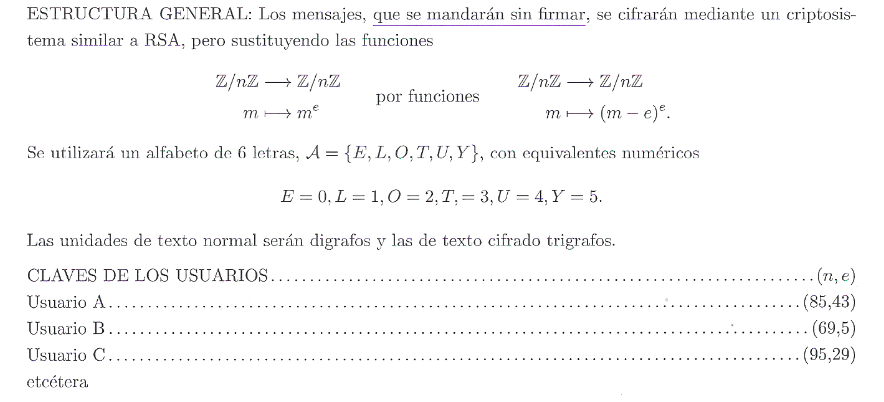
\includegraphics[width=\textwidth]{img/info_estructura_red_parcial.png}
\end{center}

Interceptamos un mensaje que el usuario $A$ ha enviado al usuario $B$, y que sabemos que termina con el nombre de $A$. El final del mensaje cifrado es $EOE$. ¿Cómo se llama el usuario $A$?
\solution

\doneby{Pedro}

% (85,43) -- (69,5)
Lo que tenemos que hacer es descifrar el mensaje $EOE$ para lo que necesitamos factorizar $n_B$.

Puesto que estamos trabajando con números pequeños es sencillo comprobar que $n_B=69 = 23\times 3$ con lo que tenemos $p=3$, $q = 23$.

A modo de comprobación, podemos ver que $e_B=5$ es coprimo con $(p-1)\cdot (q-1) = 44$.

Ahora calculamos el inverso de $e_B$:
\[d_B= \frac{1}{5} \mod 44 = 9\]

Este caso difiere un poco del caso habitual del algoritmo RSA visto en clase. Dado un mensaje $m$, el usuario $A$ envía a $B$ el valor
\[c = (m-e_B)^e_B\]
Para recuperar el valor de $m$, el usuario $B$ deberá calcular:
\[c^{d_B}+e_B = m-e_B+e_B = m\]

Una vez conocemos $e_B^{-1}$ podemos descifrar el mensaje:
\[EOE = 12 \mod 6^3 \]

\[f_{d_B}^{-1}(12) = (12)^9 + 5\mod 69 = 32 \mod 69 = 32 \mod 36 = YO\]

\end{problem}

\section{Hoja 4}
\begin{problem}[1]
 Una de las claves para que RSA funcione es el siguiente resultado:
 si $n=pq$, con $p,q$ primos distintos, y  $ed\equiv 1 \mod \phi(n)$, entonces $(m^e)^d\equiv m \mod n$ para cualquier entero $m$.

a) Sea ahora $N=mcm(p-1,q-1)$ [$mcm$=mínimo común múltiplo].
Demuestra que si  $ed'\equiv 1 \mod N$, entonces $(m^e)^{d'}\equiv
m \mod n$ para cualquier entero $m$.

b) Dados dos enteros cualesquiera $a,b$, describe un algoritmo
rápido para calcular $mcm(a,b)$, y explica por qué es rápido.
[SUGERENCIA: ¿Cuál es la relación entre $mcm(a,b), mcd(a,b)$ y
$ab$?]
\solution

\doneby{Pedro}

\spart
Puesto que $n=p\cdot q$ con $p$ y $q$ primos, sabemos que $\phi(n) = (p-1)(q-1)$.

Por definición del mínimo común múltiplo y del máximo común divisor sabemos que:
\[N=m.c.m.(p-1,q-1) = \frac{(p-1)(q-1)}{m.c.d.(q-1,p-1)}\]

Ahora sólo tenemos que ver que:
\[ed'=1\mod N \implies ed' = 1 + K\frac{(p-1)(q-1)}{m.c.d.(q-1,p-1)}\]

A partir, puesto que el $m.c.d.(p-1,q-1)$ divide tanto a $(p-1)$ como a $(q-1)$, podemos ver que,
\[\left\{ \begin{array}{l}
ed' = 1 \mod (p-1)\\
ed' = 1 \mod (q-1)
\end{array}\right.\]

Aplicando el Teorema chino del resto podemos deducir que
\[ed' = 1 \mod \left((p-1)(q-1)=\phi(n)\right) \implies (m^e)^{d'} = m \mod n\]

\spart

Podemos calcular el mínimo común múltiplo con la relación
\[m.c.m.(a,b) = \frac{ab}{m.c.d.(a,b)}\]
lo que sería muy rápido pues la multiplicación lleva tiempo $O(\log^2(N))$ y el máximo común divisor se calcula de forma rápida y sencilla con el algoritmo de euclides.

\end{problem}


\begin{problem}[2]
Encontrar la clave privada de un usuario  de un criptosistema basado en el RSA si su clave p\'ublica   es  $(7519, 35)$.

\solution

\doneby{Pedro}

Sabemos que, por definición del algoritmo RSA tenemos dos primos $p$, $q$ tales que:
\[\left\{ \begin{array}{l} 7519 = p \cdot q\\
35 = 1 \mod (p-1)(q-1)\end{array}\right.\]

Por la cuenta de la vieja podemos ver que $7519=73 \times 103$, por lo que ya conocemos $p$ y $q$.

Ahora sólo tenemos que encontrar el inverso de 35 módulo $72 \cdot 102 = 7344$ para lo que podemos emplear el algoritmo de Euclides.

\[
\begin{array}{l}
7344 = 209\cdot 35 +29\\
35 = 1 \cdot 29 + 6 \\
29 = 4\cdot 6 + 5 \\
6 = 5 + 1
\end{array} \implies \begin{array}{l}
1 = 6 - 5 \\
5 = 29 - 4 \cdot 6 \implies 1 = 5 \cdot 6-29\\
6 = 35 - 29 \implies 1 = 5\cdot 35 -6 \cdot 29 \\
29 = 7344 - 209 \cdot 35 \implies 1=1259 \cdot 35 -6\cdot 7344
\end{array}
\]

Así tenemos que la clave privada es $d=1259$

\end{problem}

\begin{problem}[3]
En la guía de una red de comunicaciones aparece la siguiente
información:

ESTRUCTURA GENERAL: Los mensajes se cifrarán mediante el
criptosistema RSA. Se utilizará el alfabeto castellano de 30
letras  con 0,\dots,14,\dots,26=A,\dots,Ñ,\dots,Z, 27=el punto,
28=espacio en blanco y 29=la interrogación. Las unidades de texto
normal serán digrafos y las de texto cifrado trigrafos. Los mensajes se mandan
{\bf sin firma}.

 CLAVES DE LOS
USUARIOS\dotfill$(n,e)$

Usuario A\dotfill(1711,125)

etcétera
\vspace{2mm}

  El usuario B envía el mensaje {\it ASÑAW.} al usuario A.   ¿Qué quiere decirle B a A?
\solution

\doneby{Pedro}

Lo que debemos hacer es encontrar los primos $p,q$ con los que se diseñó este sistema RSA.

Por la cuenta de la vieja llegamos a que $1711=p\cdot 1 = 29 \cdot 59$.

Una vez tenemos esto podemos conocer $(p-1)\cdot (q-1)=28 \cdot 58 = 1624$ lo que nos permite calcular la clave privada, que, en este caso, es el inverso de 125 módulo $1624$. Vamos a ello

\[
\begin{array}{l}
1624 = 12 \cdot 125 + 124\\
125 = 124 + 1
\end{array} \implies \begin{array}{l}
1 = 125 -124 \\
124 = 1624 - 12 \cdot 125 \implies 1 = 13 \cdot 125 - 1624
\end{array}
\]

Así tenemos que la clave privada, empleada para descifrar, será $d=13$.

Para descifrar el mensaje procedemos por bloques:
\[19\cdot 30 + 14 = 584 \mod 1711 \to 584^{13} \mod 1711 = 225 = 7\cdot 30 + 15 = HO\]
\[23 \cdot 30 + 27 = 717 \mod 1711 \to 717^{13} \mod 1711 = 330 = 11 \cdot 30 + 0 = LA\]

Así tenemos que el mensaje enviado era ``HOLA''
\end{problem}

\begin{problem}[4]
En la guía de una red de comunicaciones aparece la
siguiente información:

ESTRUCTURA GENERAL: Los mensajes se cifrarán mediante el
criptosistema RSA. Se utilizará el alfabeto castellano de 26
letras (con Ñ y sin W). Las unidades de texto normal serán
digrafos y las de texto cifrado trigrafos. Los mensajes se mandan
{\bf firmados} (usando el protocolo explicado en clase).

 CLAVES DE LOS
USUARIOS\dotfill$(n,e)$\hphantom{(9797,17)(8549,6083)}

Usuario A\dotfill(9797,17)\hphantom{$(n,e)$(8549,6083)}

Usuario B\dotfill(8549,6083)\hphantom{(9797,17)$(n,e)$}

etcétera
\vspace{2mm}


  El usuario A envía un mensaje al usuario B y lo termina con
la firma EOBIXD. ?`Cómo se llama el usuario A?
\solution

\doneby{Pedro}

Para saber cómo se llama el usuario $A$ lo que tenemos que hacer es descifrar el mensaje para lo que debemos atacar al sistema RSA.

Procedemos a factorizar $n_B$ por la cuenta de la vieja obteniendo
\[n_B= 83 \cdot 103 = p \cdot q\]

A partir de aquí podemos calcular la clave privada calculando:
\[\frac{1}{e_b} \mod (p-1)(q-1) \equiv \frac{1}{6083} \mod 8364\]

Empleamos el algoritmo de Euclides para calcular este inverso:

\[
\begin{array}{l}
8364 = 1 \cdot 6083 + 2281 \\
6083 = 2\cdot 2281 + 1521 \\
2281 = 1\cdot 1521 + 760 \\
1521 = 2 \cdot 760 + 1
\end{array} \implies \begin{array}{l}
1 = 1521 -2\cdot 760 \\
760 = 2281 - 1521 \implies 1 = 3\cdot 1521 -2\cdot 2281 \\
1521 = 6083 - 2\cdot 2281 \implies 1 = 3 \cdot 6083 -8 \cdot 2281 \\
2281 = 8364 - 6083 \implies 1 = 11 \cdot 6083 - 8 \cdot 8364
\end{array}
\]

Por tanto tenemos que $d_B=11$.

Puesto que el mensaje ha sido firmado lo que hemos recibido es
\[\algb{C}=f_{d_A}(f_{e_B}(\algb{M}))\]

luego para descifrarlo debemos emplear primero la clave pública de $A$ y luego la privada de $B$, que acabamos de descubrir.

Una vez sabemos esto podemos descifrar el mensaje:
\[\begin{array}{l}
EOB = 3095 \mod n_A \to 3095^{17} \mod n_A = 1431 \mod n_A \to 1431^{11} \mod n_B = 255\\
255 = 9 \cdot 26 + 21 = ``JU''\\
IXD = 6009 \mod n_A \to 6009^{17} \mod n_A = 1954 \mod n_A \to 1954^{11} \mod n_B = 12\\
12 = 0 \cdot 26 + 12 = ``AN''
\end{array}\]


\end{problem}


\begin{problem}[5]
Un grupo de espias decide cifrar sus mensajes, escritos en
un alfabeto de 27 letras (las 26 del castellano, con Ñ y sin W, y
un espacio en blanco ``\_" que cifrarán como el 26), utilizando un
sistema de Vigenére sobre pares de letras. Para dificultar la
labor del enemigo, y en particular el análisis de frecuencias,
deciden cambiar la clave en cada mensaje. Para intercambiarse las
claves acuerdan utilizar el sistema RSA de clave pública. El
protocolo que utilizan es el siguiente:

Cuando $A$ quiere enviar a $B$ un mensaje $m$, busca una clave de
Vigenére, $K$, que será un par de letras $k_1k_2$. Esta clave le
da una función para cifrar $g_K$. Además $B$ tiene una función
pública para cifrar claves, $f_B$, cuya correspondiente función
para descifrar, $f^{-1}_B$, es secreta. $A$ interpreta $K$ (en
principio un par de letras) como un digrafo (un ``número de dos
cifras") al que puede aplicar $f_B$, y lo que envía a $B$ es el
par $(f_B(K),g_K(m))$. $B$ puede recuperar $K$ a partir de
$f_B(K)$, y una vez que conoce $K$ puede leer $m$ a partir de
$g_K(m)$.

\ppart Si las claves para cifrar son de la forma $(n,e)$, ?`Hay alguna
restricción sobre el tamaño de $n$?

\ppart Las primeras lineas de la guía de claves públicas para cifrar
claves de Vigenére dicen:

 Usuario
A\dotfill$((3^9-1)/2,3629)$\hphantom{$((2^{15}-1)/49,643)$$((3^9-1)/2,3629)$}


Usuario
B\dotfill$((2^{15}-1)/7,643)$\hphantom{$((3^9-1)/2,3629)$$((3^9-1)/2,3629)$}

 El usuario $B$ recibe el mensaje (AGR, TPXUROXK\_X). ?`Qué le han
querido decir?

\ppart Como acabas de comprobar, el protocolo anterior tiene un serio
problema de autentificación: cualquiera podría haber enviado el
mensaje. Discute si para resolver este problema es suficiente que
cuando $A$ escribe a $B$ envie el mensaje en la siguiente forma:
(Hola soy $A$, $f^{-1}_A(f_B(K)),g_K(m)$); o si hace falta
introducir alguna firma adicional. Discute también si siempre se
podrá utilizar $f^{-1}_A(f_B(K))$ o si habrá casos en los que
convenga sustituirlo por $f_B(f^{-1}_A(K))$. ?`Introduce esta
modificación alguna nueva restricción sobre el tamaño de las
posibles $n$ de las claves?

\ppart Supón que los espias han decidido cambiarse al nuevo protocolo
descrito en c), y que quien envió el mensaje de b) fue $A$. ?`Como
debería enviar ese mismo mensaje con el nuevo protocolo?
\solution

\doneby{Pedro}

\spart

La clave $k_1k_2$ se interpretará como un número en $\ent_{27^2}$.

Puesto que para cifrar este dato mediante el algoritmo RSA tendremos que calcular su módulo $n$, necesitaremos que $n>27^2$ pues, de lo contrario, tendríamos dos claves distintas en claro que podrían llevar a la misma clave cifrada.

\spart

Para empezar debemos factorizar el $n_B$.

Para todo factor primo tenemos distinto de $7$, que sabemos que es factor, tenemos:
\[p|2^{15}-1 \implies \left\{ \begin{array}{l}
p|(2^1-1)\implies \text{ imposible}\\
p|2^3-1 \implies p|7 \implies p=7\\
p|2^5-1 \implies p |31 \implies  p=31\\
p =1 \mod 30 \end{array}\right.\]

Así tenemos que
\[\frac{2^{15-1}}{7} = 31\cdot 151 = p\cdot q\]

Ahora, para descifrar el mensaje debemos calcular el inverso de $e_b$ en módulo $(p-1)(q-1)$, es decir, debemos calcular:
\[\frac{1}{643} \mod 4500\]

Como siempre, empleamos el algoritmo de Euclides
\[
\begin{array}{l}
4500 = 6 \cdot 643 + 642\\
643 = 642 + 1
\end{array} \implies \begin{array}{l}
1 = 643 - 642 \\
642 = 4500 - 6 \cdot 643 \implies 1 = -4500 + 7\cdot 643
\end{array}
\]

Con esto procedemos a descifrar el mensaje:

\[\begin{array}{l}
AGR = 180 \mod n_B \to 180^{7} \mod n_B = 521 \mod 151\cdot 31 = 521 \mod n_A \\
521 = 19 \cdot 27 + 8
\end{array}\]

Una vez tenemos $k_1,k_2=19,8$ procedemos a descifrar el mensaje $m$ obteniendo:
\[TPXUROXK\_X \to BIEN\_HECHO\]
\newpage

\spart

El nuevo sistema descrito nos permite garantizar la autoría del mensaje puesto que sólo el usuario $A$ conoce $f_A$.

Puesto que ahora vamos a cifrar con $f_A^{-1}$ el total del mensaje y calcularemos $\mod n$ de ese valor, necesitaremos que $n$ sea mayor que $27^N$ siendo $N$ la longitud máxima de mensaje que vamos a definir.

\spart

Para por ver como se enviaría el mensaje con el nuevo protocolo debemos calcular la clave privada de $A$ y cifrar todo el mensaje con ella.

Procedemos a factorizar $n_A$.

Para todo factor primo tenemos distinto de $2$, que sabemos que es factor, tenemos:
\[p|3^{9}-1 \implies \left\{ \begin{array}{l}
p|3^3-1\implies p|26 \implies p =13 \Or p=2\\
p =1 \mod 18 \end{array}\right.\]

Así tenemos que
\[\frac{3^9-1}{2} = 13 \cdot 757\]

Llegados a este punto deberíamos intentar factorizar el $757$ pero, puesto que sabemos que estamos trabajando con un algoritmo RSA, sabemos que $\frac{3^9-1}{2}=p\cdot 1$ por lo que $757$ ha de ser primo.

Ahora calculamos el inverso de $e_A \mod n_A$, es decir:
\[\frac{1}{3629} \mod 9072\]

Vamos a ello
\[
\begin{array}{l}
9072 = 2 \cdot 3629 + 1814\\
3629 = 2\cdot 1814 + 1
\end{array} \implies \begin{array}{l}
1 = 3629 - 2 \cdot 1814 \\
1814 = 9072 - 2 \cdot 3629 \implies 1 = -2\cdot 9072 + 5\cdot 3629
\end{array}
\]

Con esto procedemos a descifrar el mensaje, puesto que al ser $n=3629$ sabemos que el tamaño máximo del bloque es 2. (Lógicamente no tiene sentido que se usen bloques de una sóla letra, por lo que entendemos que los bloques son de longitud 2)

Puesto que el mensaje tiene un número de letras que no es múltiplo de 2, éste deberá ser completado de alguna forma previamente definida antes de ser cifrado.

\end{problem}


\begin{problem}[6]
Supongamos que el alfabeto en claro tiene $29$ letras con
0,...,26=A,...,Z [alfabeto castellano], 27=espacio en blanco,
28=el punto, y que el alfabeto cifrado tiene $30$ letras,
añadiendo al anterior 29=?.   Las unidades de texto en claro serán
digrafos vistos como números de dos cifras en base $29$, es decir,
enteros entre $0$ y $840$ [o elementos de $\ent_{841}$].
Análogamente, las unidades de texto cifrado serán digrafos vistos
como enteros entre $0$ y $899$ [o elementos de $\ent_{900}$].
\begin{itemize}
\item[a)] El cifrado de $m$ es un entero $0\le f(m)\le  850$ tal que
$$f(m):=m^{13}+2 \pmod {851}.$$ (Notar que $(29)^2<851<(30)^2$.)
 Descifra el mensaje {\it LFNÑ}.
\item[b)]  ¿Es posible usar $g(m):=m^{11}+2 \pmod{851}$ para cifrar?
\end{itemize}
\solution

\doneby{Pedro}

\spart

Para poder descifrar la clave podemos suponer que estamos trabajando con un sistema $RSA$ (una vez le restemos 2 al mensaje cifrado estaremos ante un sistema RSA literalmente) con clave pública $e=13$ y $n=851$.

Procedemos a factorizar $851=p\cdot q = 37 \cdot 23$ por la cuenta de la vieja.

Ahora procedemos a calcular la clave privada:
\[d=\frac{1}{13} \mod 792 = 61\]

En esta ocasión es fácil ver que si multiplicamos por $13\cdot 60$ andamos cerca de $792$ y probando vemos rápido cuál es el inverso.

Para quien no lo vea así de rápido siempre puede aplicar el algoritmo de Euclides.

Una vez conocemos la clave de descifrado procedemos a descifrar el mensaje:
\[\begin{array}{l}
LF = 335 \mod 851 \to 335^61 \mod 851 = 37 = ``BI''\\
N\tilde{N} = 404 \mod 851 \to 404^{61} \mod 851 = 129 = ``EN''
\end{array}\]

\spart

Podemos ver que no es posible emplear la función $g$ para cifrar puesto que
\[(p-1)(q-1) = 792 = 11\cdot 72\]

Por tanto, si tratásemos de emplear esta función para cifrar, al tratar de encontrar la clave privada veríamos que es imposible puesto que $e=11$ no es coprimo con $(p-1)(q-1)$.

 \end{problem}

\begin{problem}[7]
Supongamos que el alfabeto en claro tiene $29$
letras con 0,...,26=A,...,Z [alfabeto castellano], 27=espacio en
blanco, 28=el punto, y que el alfabeto cifrado tiene $30$ letras,
añadiendo al anterior 29=?   Las unidades de texto en claro serán
digrafos vistos como números de dos cifras en base $29$, es decir,
enteros entre $0$ y $840$ [o elementos de $\ent_{841}$].
Análogamente, las unidades de texto cifrado serán digrafos vistos
como enteros entre $0$ y $899$ [o elementos de $\ent_{900}$].
\begin{itemize}
\item[a)]  El cifrado de $m$ es un entero $0\le f(m)\le  852$ tal que
$$f(m):=m^{31}+2 \pmod {853}.$$ (Notar que $(29)^2<853<(30)^2$.)
 Descifra el mensaje {\it .CZE}
\item[b)]  ¿Es posible usar $g(m):=m^{32}+2 \pmod{853}$ para cifrar?
\end{itemize}
\solution
\doneby{Edu}

\spart
En primer lugar observamos que 853 es primo\footnote{No es divisible por ningún primo en $\set{p \tq p \in \set{\text{primes}}, p \leq \sqrt{853} \leq 30} = \set{2,3,5,7,11,13,17,19,23,29}$; y SAGE opina lo mismo.} y podría entrar la duda si podremos resolver el problema. La respuesta es que aunque RSA diga que $n = p \cdot q$ es un requisito, en realidad solo necesitamos que se pueda aplicar el Pequeño Teorema de Fermat (\ref{thm:FermatsLittleTh}) y el Teorema Chino del Resto.

Por tanto, buscamos un $d$ tal que $e \cdot d = 1 \mod \varphi(853)$. Como 853 es primo, $\varphi(853) = 852$.

Procedemos al cálculo de $d$ usando el Algoritmo de Euclides Extendido:
\begin{gather*}
852 = 27 \cdot 31 + 15\\
31 = 2 \cdot 15 + 1\\
1 = 55 \cdot 31 - 2 \cdot 852
\end{gather*}

Por tanto, $d = 55$; que en binario es $110111$, y nuestra función inversa queda $f^{-1}_{d}(y) = (y - 2)^{55} \mod 853$, con $y = f_{e}(x)$ para algún $x$.



Pasemos a descifrar. En primer lugar, pasamos el texto a números:

``.C'' $= 28 \cdot 30 + 2 = 842$

``ZE'' $= 26 \cdot 30 + 4 = 784$

Por lo que tenemos que calcular:
\begin{gather*}
(842-2)^{55} \mod 853\\
(784-2)^{55} \mod 853
\end{gather*}

Aplicamos el método de exponenciación binaria modular para calcular la potencia 55 en el primer caso:
\begin{gather*}
840^{2} \mod 853 = 169, \quad 840^{4} \mod 853 = 412\\
840^{8} \mod 853 = 850, \quad 840^{16} \mod 853 = 9\\
840^{32} \mod 853 = 81\\
840^{3} \mod 853 = 840 \cdot 840^{2} \mod 853 = 362\\
840^{7} \mod 853 = 840^{3} \cdot 840^{4} \mod 853 = 722\\
840^{23} \mod 853 = 840^{7} \cdot 840^{16} \mod 853 = 527\\
840^{55} \mod 853 = 840^{23} \cdot 840^{32} \mod 853 = 37\\
\end{gather*}
Y como $37 = 1 \cdot 29 + 8$, obtenemos ``BI'', como primera unidad de texto en claro.

Y repitiendo el proceso en el otro caso obtenemos $782^{55} \mod 853 = 129 = {4 \cdot 29 + 13}$, que en texto es ``EN''.

Juntándolo todo, el texto en claro es ``BIEN''.

\spart

No será posible emplear la función $g$ puesto que al calcular el inverso de $32$ tendríamos que calcular el inverso de $32$ en $\ent_{852}$ pero $(32,852) \neq 1$ por lo que no tendrá inverso.
\end{problem}

%\begin{problem}
% Al cifrar los mensajes mediante el criptosistema RSA el primer número de las claves de los usarios $(n,e)$  es producto de 2 primos.

%1) ¿Porqué $n$ no puede ser un número primo?
%Porque factorizarlo sería muy fácil (los tests de primalidad son más rápidos que factorizar), luego si publicas (n,e), calcular d sería superrápido con el algoritmo de Euclides.

%2) ¿Porqué no se usan claves con $n$ igual a producto de 3 primos?
% Sí que se puede, se llama Multiprime-RSA. http://crypto.stackexchange.com/a/5692
%\end{problem}


\begin{problem}[8]
Probar que 15 es un pseudo-primo en base 4,
que 28 es un pseudo-primo en base 9 y que 91 es un pseudo-primo en
base 3.
\solution
\doneby{Edu}

\spart
Vamos a ver que esos números son pseudoprimos para las bases dadas:

En primer lugar, vemos que $(15,4) = 1$.

En segundo lugar, calculamos $4^{(15-1)} \mod 15$. Como $14 = 1110$ en base 2:
\[
4^2 = 1 \mod 15, 4^4 = 1 \mod 15, 4^8 = 1 \mod 15
\]

luego $4^14 = 4^8 \cdot 4^4 \cdot 4^2 = 1 \cdot 1 \cdot 1 = 1 \mod 15 $ por lo que vemos que efectivamente da 1, luego 15 es pseudoprimo en base 4.

\spart

Comprobamos que $(28,9)=1$.

Calculando $9^{27} \mod 28$ comprobamos que efectivamente da 1.
$27$ en binario es $11011$:
\[ 9^2 = 25 \mod 28, 9^4 = 9 \mod 28, 9^8 = 25 \mod 28, 9^{16} = 9 \mod 28\]

Luego $9^{27} \mod 28 = 9 \cdot 25 \cdot 25 \cdot 9 = 1 \mod 28$, así que efectivamente, 28 es un pseudoprimo en base 9.

\spart

Nos cercioramos de que $(91,3) = 1$.

Y tenemos que calcular: $3^{90} \mod 91$. Que efectivamente, da 1. % fiaros de mi

\end{problem}

\begin{problem}[9]
Sea $n$ un número impar compuesto y sea $(b,n)=1$.

\ppart Sea $p$ un divisor primo de $n$ y escribamos $n'=n/p$. Probar que si $n$
es un pseudo-primo en base $b$ entonces $b^{n'-1}\equiv 1 \mod p$.

\ppart Demostrar que ningún entero de la forma $n=3p$, con $p>3$
primo, puede ser un pseudo-primo en bases 2, 5 ni 7.

\ppart Demostrar que ningún entero de la forma $n=5p$, con $p>5$
primo, puede ser un pseudo-primo en bases 2, 3 ni 7.

\ppart Probar que 91 es el menor pseudo-primo (impar) en base 3.

\solution

\doneby{Pedro}

\spart

Si $n$ es pseudoprimo en base $b$ sabemos que
\[b^{n-1} = 1 \mod n \implies b^{n-1}=1 \mod p \text{ puesto que } p|n\]

Por tanto tenemos que
\[b^{n'-1} = b^{\frac{n-p}{p}} \mod p =\footnote{Por el pequeño teorema de Fermat $a^p=a \mod p$ siendo $p$ un primo cualquiera} \left(b^{\frac{n-p}{p}}\right)^p \mod p\]

Asi tenemos:
\[b^{n'-1} \mod p= b^{n-p} \mod \frac{b^n}{b^p} \mod n = \frac{b^n}{b} \mod n = b^{n-1} \mod p = 1\]

\spart

Por el apartado $a)$ sabemos que si $n$ fuese pseudoprimo en base $b$, siendo $n=3 \cdot p$ tomando $n'=3$ deberíamos ver que $b^{n'-1}=1 \mod p$.

Sin embargo, en este caso tenemos:
\[2^{3-1} = 4=2^2 \mod p\]
\[5^{3-1} = 25=5^2\mod p\]
\[7^{3-1} = 49=7^2 \mod p\]

Recordemos que si tenemos una ecuación de la forma
\[a^2=1 \mod p\]
siendo $p$ un número primo, puesto que nos estamos moviendo en un cuerpo, necesitamos que $a=1$ ó $a=p-1$.

En los casos que tenemos en este ejercicio es obvio ver que $a\neq 1$ y, en caso de tener $a=p-1$ necesitaríamos que $p$ fuese 3,6 y 8 respectivamente.

El 3 es primo pero no cumple la condición de ser estrictamente mayor que 3 y las otras dos posibilidades no son valores primos.

En definitiva, no hay ningún primo $p>3$ que haga que $n=3p$ sea pseudoprimo en las bases 2,5 o 7.

\spart

Con la misma idea del apartado anterior tenemos:
\[2^{5-1} = 16=4^2 \mod p\]
\[3^{5-1} = 81=9^2 \mod p\]
\[7^{5-1} = 2041=49^2 \mod p\]

Si tuviésemos que, en alguno de los casos anteriores:
\[a^2 =1 \mod p\]
Ya hemos visto que necesitamos que $a=1$ ó $a=p-1$

Puesto que 10 y 50 no son primos y 5 no es estrictamente menor que $5$, es claro que no hay ningún primo $p$, con las condiciones iniciales dadas, que haga que $n=5p$ sea primo en bases 2,3 ni 7.

\spart {\color{red}Jorge: creo que está mal (yo no se cómo resolverlo)}

Podemos representar un número impar de forma general como $n=2k+1$. Si este número fuese pseudoprimo en base 3 tendríamos que:
\[3^{2k} = 1 \mod (2k+1)\]

Por el apartado $b)$ sabemos que ningún múltiplo de $5$ será pseudoprimo en base $3$ ({\color{red} esto es mentira, lo que dice el apartado b) es que ningún producto de un primo por $5$ será pseudoprimo, pero no dice nada de múltiplos de 5 en los que no multiplicamos por un primo, como $20=5·4$}). Además, es sencillo ver que si $n=3p$ entonces
\[3^{3p-1}=1 \mod 3p \implies 3^2 =1 \mod p \iff p=2\]

{\color{red} esta línea es mentira porque tomando $p=2$ queda $3^5\equiv3\not\equiv1 \mod 6$}

Por tanto tendremos que el $6$ es pseudoprimo en base 3, pero en este apartado nos estamos restringiendo a los números impares por lo que esto no nos interesa.

Hasta ahora, ya hemos probado que ni los múltiplos de 3 ni los múltiplos de 5 son pesudoprimos en base 3. Si demás eliminamos a los números primos, puesto que estos no son considerados pseudoprimos, tendremos muy pocos posibles números impares menores que 91 con los que debemos probar hasta obtener el primer pseudoprimo en base 3.

La lista de candidatos, recordando que sólo nos interesan los impares, queda como:
\[\{49, 77, 91\}\]

que es perfectamente manejable y sencilla de probar
\end{problem}

\begin{problem}[10]
\ppart Probar que si $2^n-1$ es primo entonces $n$ es primo, y que si
$2^n+1$
 es primo entonces $n=2^k$. Los números $M_p:=2^p-1$, con $p$ primo, se
llaman ``números de Mersenne"\ y ``primos de Mersenne"\ en caso de
ser primos. Los de la forma $F_k:=2^{2^k}+1$ se llaman\ ``números
de Fermat"\ y\ ``primos de Fermat"\ si son primos. Los primeros
primos de Mersenne son 3,7, 31, 127, y todos los primos de Fermat
conocidos son 3, 5, 17, 257 y 65537.

\ppart Probar que todos los números de Fermat y todos los números de
Mersenne son pseudo-primos en base 2. (SUGERENCIA: Para los
números de Fermat, estudiar primero $2^{2^k} \mod F_k$, y
comprobar que podemos calcular $2^{F_k}$ a partir de este valor
por iteración de cuadrados. Para los de Mersenne, empezar por ver
que $p\vert M_p-1$ y deducir de ello que $M_p= 2^p-1\vert
2^{M_p-1}-1$.)

\ppart A pesar de lo anterior, comprobar que uno puede ver que $M_{11}=2047$ no es
primo utilizando un sencillo test de primalidad.

\solution

\doneby{Pedro}

\spart
\begin{itemize}
\item \textbf{Demostramos que si $2^n-1$ es primo entonces lo es $n$}

\doneby{Jorge}

Por lo visto en teoría, en la proposición \ref{prop:pbn-1}, sabemos que si $p|2^n-1$ entonces ó bien $p|2^d-1$  con $d|n,\ d<n$, ó bien $p=1 \mod n$.

Tomemos $p=2^n-1$ y supongamos $n$ no primo, entonces sabemos que $n$ tiene algún divisor $d|n$ con $d<n$, y por la proposición \ref{prop:pbn-1} tenemos $p|2^d-1 < 2^n-1$. Sin embargo en nuestro caso tenemos precisamente $p=2^n-1$, con lo que llegamos a la contradicción de que $2^n-1< 2^n-1$.


\item \textbf{Demostramos que si $2^n+1$ es primo entonces $n$ es potencia de 2}
\footnote{Demostración sacada de \href{https://en.wikipedia.org/wiki/Fermat_number\#Other_theorems_about_Fermat_numbers}{Wikipedia}}

Si $n$ es un número positivo que no es potencia de 2, debe tener un factor impar $s>2$, por lo que podemos escribir
\[n = r\cdot s \ \text{ con } 1 \leq r < n\]
Por otro lado sabemos que $(a-b)|(a^m-b^m)$ (\href{https://en.wikipedia.org/wiki/Fermat_number\#Other_theorems_about_Fermat_numbers}{Wikipedia}). Si tomamos $a=2^r$, $b=-1$ y $m=s$ tenemos que
\[(2^r+1)|2^{rs}+1 \text{ puesto que s es impar} \implies (2^r+1)|2^n+1\]
es decir, llegamos a que $2^n + 1$ no es primo.

Queda claro por tanto que $n$ no puede tener ningún divisor impar y, por tanto, ha de ser potencia de 2.
\end{itemize}
\spart

\begin{itemize}
\item \textbf{Demostramos que los números de Fermat son pseudoprimos en bse 2}

Decimos que un número es un \concept{número de Fermat} si $F_k=2^{2^k}+1$.

Atendiendo a la indicación del enunciado vemos que
\[2^{2^k} \mod F_k = -1 \mod F_k\]

Si queremos ver que $F_k$ es pseudoprimo en base 2 debemos ver que
\[2^{F_k-1} = 1 \mod F_k \equiv 2^{2^{2^k}} = 1 \mod F_k\]

Atendiendo al valor de $2^{2^k} \mod F_k$, podemos ver que si multiplicamos este valor por si mismo $2^{2^k-k}$ veces obtenemos:
\[\left(2^{2^k}\right)^{2^{2^k-k}} = 2^{2^k\cdot 2^{2^k-k}} = 2^{2^{2k}} = 1 \mod F_k \text{ puesto que } 2^α \text{ es par}\]

Con lo que queda claro que $F_k$ es pseudoprimo en base 2.

\item \textbf{Demostramos que los números de Mersenne son pseudoprimos en bse 2}

Atendiendo a la sugerencia del enunciado vemos que
\[M_p-1=2^{p}-2=2(2^{p-1}-1)\]

Recordando nuevamente la proposición \ref{prop:pbn-1} tenemos que si $p=1 \mod n$ entonces $p|2^n-1$. En este caso tenemos que $n=p-1$ por lo que $p$, evidentemente satisface la condición, pues
\[p = 1 \mod p-1\]

Recordando una idea del apartado anterior tenemos que
\[(a-b)|(a^m-b^m)\]
si tomamos $a=2^p$, $b=1$ y $m=\frac{M_p-1}{p}$ (que sabemos que es un entero pues acabamos de demostrar que $p|M_p-1$) nos queda
\[2^p-1 | 2^{M_p-1}-1\]
que es justo lo que queríamos demostrar.

\end{itemize}


\spart

Podemos explotar que $2047 = 2^{11} - 1$ y aplicar \ref{prop:pbn-1}. De hecho, este es el ejemplo que vimos.
\end{problem}

%\begin{problem}
%Sea $n$ un número de Carmichael. Demostrar que

%a) $n$ no es divisible por $m^2$ para ningun $m>1$;

%b) $n-1$ es divisible por $p-1$ para cualquier divisor primo $p$de $n$;

%c) $n$ es divisible por lo menos por 3 primos.
%\end{problem}

\begin{problem}[11]
\ppart Prueba que los siguientes son números de Carmichael: 561,
1729, 2465, 41041, 825265.

\ppart Demuestra que 561 es el menor número de Carmichael.

\solution

\doneby{Pedro}

\spart
Recordemos que un número es de Carmichael es aquel número \textbf{compuesto}, $n$, tal que $b^{n-1}=1 \mod n$ para todo $b$ coprimo con $n$.

Vamos a comprobar que los números dados son de Carmichael comprobando, con el ordenador, que se satisfacen las ecuaciones necesarias. A continuación mostramos la factorización de cada uno de los números a estudiar

\[ \left\{\begin{array}{l}
561 = 11 \cdot 51 = 11 \cdot 17 \cdot 3\\
1729 = 7 \cdot 247 = 7 \cdot 13 \cdot 19\\
2465 = 5 \cdot 493 = 5 \cdot 17 \cdot 19\\
825265 = 5 \cdot 165053 = 5 \cdot 7 \cdot 23579 = 5 \cdot 7 \cdot 17 \cdot 1387 = 5 \cdot 7 \cdot 17 \cdot 19 \cdot 73
\end{array}\right.\]

\spart

Esta demostración parece ser un Kaos al punto de que es más fácil probar por fuerza bruta que cascarse algunas demostraciones que he encontrado por internet.

Os dejo esta como ejemplo: \href{http://math.stackexchange.com/questions/433029/the-smallest-example-of-a-carmichael-number}{Prueba de que 561 es el menor número de Carmichael}

\textbf{Solución en clase:}

Sabemos que los números de Carmichael tienen, al menos, 3 factores primos y que no tiene factores repetidos. (El \textbf{Teorema de Korset} nos lo garantiza). Además podemos descartar el 2 como factor, como demostraremos en el ejercicio 13 de esta sección.

El menor número posible que tenga 4 factores primos distintos es el número $n=3\cdot 5 \cdot 7 \cdot 11 > 561$, luego sabemos que los posibles números de Carmichael menores que 561 tendrán sólo tres factores primos.

Con esta idea podemos reducir la cantidad de candidatos posibles, al punto de poder probar a mano.

\end{problem}

\begin{problem}[12]
 Supongamos que $m$ es un entero positivo tal que $6m+1$, $12m+1$
y $18m+1$ son todos primos. Demostrar que $n=(6m+1)(12m+1)(18m+1)$
es un número de Carmichael. (Esta idea es una de las que han sido
utilizadas para intentar demostrar que hay infinitos números de
Carmichael, y durante mucho tiempo fue el método utilizado para
encontrar números de Carmichael muy grandes.)
\solution

Sabemos que $n=p_1\cdot p_2\cdot p_3$, con $p_i$ primos, será un número de Carmichael si y sólo si $p_i-1|n-1$, por el \textbf{criterio de Korset}

Lo que tenemos que hacer es demostrar que $6m,12m$ y $18m$ divide a $n-1$. En concreto basta con ver que $2^2,3^2,m$ dividen a $n-1$.

Es decir, debemos comprobar que $n=1 \mod 2^2,3^2,m$. Vamos a ello:

\[n \mod m = (6m+1 \mod m)(12m+1\mod m)(18m +1 \mod m) = 1 \mod m\]
\[n \mod 4 = (2m+1)(1)(2m+1) \mod 4 = 4m^2+4m+1 \mod 4 = 1 \mod 4\]
\[n \mod 9 = (6m +1 )(3m+1) (1) \mod 9 = 1-9m^2 \mod 9 = 1 \mod 9\]


\end{problem}

\begin{problem}[13]
Dado que es muy facil saber si un número par es primo o no (el
único par primo es el 2), no tiene demasiado sentido aplicar tests
de primalidad a los números pares. Sin embargo, y por aquello de
tener una teoría completa, se pide: demostrar que no existen
números de Carmichael pares, o sea, que para todo $n$ par existe
$b$ tal que $(b,n)=1$ y $b^{n-1}\not\equiv 1\mod n$.

\solution

\doneby{Pedro}

La demostración es bien sencilla pues basta con tomar $b=n-1$.

Así tenemos que $n-1$ y $n$ son coprimos, pues en caso de tener un factor común, tendríamos:
\[p|n \y p|n-1 \implies p|(n-(n-1)) \implies p| 1 \implies p=1\]

En este caso tendríamos
\[(n-1)^{n-1} \mod n = (-1)^{n-1} \mod n = -1 \mod n \neq 1 \mod n\]

donde la última desigualdad se basa en que $n-1$ será impar, puesto que $n$ es par.

\end{problem}

\begin{problem}[14]
Recordemos que la existencia de infinitos números de Carmichael es
un resultado reciente (Alford, Granville, Pomerance 1992). Sin
embargo, la existencia de infinitos pseudo-primos (verdaderos, o
sea, no primos) en base 2 era bien conocida. Posiblemente la
demostración más simple es la siguiente (Malo 1903): probar que si
$n$ es un pseudo-primo en base 2 compuesto, entonces $n':=2^n-1$
también es un pseudo-primo en base 2 compuesto. (SUGERENCIA: Tanto
la composición como la pseudo primalidad se basan en el hecho de
que si $a\vert b$ entonces $2^a-1\vert 2^b-1$, y en observar que
si $n$ es pseudo-primo en base 2 entonces $n\vert n'-1$.)
\solution

\doneby{Pedro}

Si $n$ es un pseudoprimo en base 2 tenemos que $2^n=2 \mod n$. A partir de esta información queremos demostrar que
\[2^{2^n-1}=2 \mod 2^n-1 \equiv 2^{2^n-2} = 1 \mod 2^n-1\]

Sabiendo que $n$ es pseudoprimo en base 2 tenemos que:
\[n|n'-1 \iff n| 2^n-2 \iff n|kn \text{ donde usamos que } 2^n=2 \mod n\]
Con lo que tenemos que $n|n'-1$.

Atendiendo de nuevo a la sugerencia del enunciado vemos que, dado que $n|n'-1$ sabemos que:
\[2^n-1 | 2^{2^n-2}-1 \implies 2^{2^n-2}-1 = 0 \mod 2^n-1 \implies 2^{2^n-1} = 1 \mod 2^n-1\]
que es justo lo que queríamos demostrar.

\end{problem}

\begin{problem}[15]
\ppart Encontrar los valores de $b$ para cuales $21$ es
pseudoprimo fuerte en base $b$.

\ppart  Encontrar los valores de $b$ para cuales $35$ es
pseudoprimo fuerte en base $b$.

\solution

\doneby{Pedro}

Recordemos que dado $n \in \ent$ impar con $n>9$ y $n-1=r2^s$ siendo $r$ impar y $s \geq 1$, diremos que $n$ es \textbf{pseudoprimo fuerte} en base $b$ si $(n,b)=1$ y o bien:
\[b^r=1 \mod n\]
o bien para algún $0 \leq i \leq s-1$ se cumple
\[b^{r2^i}=-1\mod n\]

\spart

En este caso tenemos $n-1=20 =5\cdot 2^2$, por lo que tenemos $r=5$.

Si tenemos que 21 es pseudoprimo en base $b$ tenemos como posibles valores de $b$ aquellos números coprimos con 21, es decir
\[b\in \{2,4,5,8,10,11,13,16,17,19\}\]

Para ninguno de estos valores se satisface la condición $b^r=1 \mod n$.

La segunda condición nos da la posibilidad de que $b^2r=1 \mod n$ para considerar $b$ como pseudoprimo fuerte.

Nuevamente no obtenemos ningún resultado, es decir, $21$ no es pseudoprimo fuerte en ninguna base.

\spart

En esta ocasión tenemos $n-1=34=17\cdot 2$ con lo que tenemos $r=17$.

Los posibles candidatos son:
\[\{2,3,4,6,8,9,11,12,13,16,17,18,19,22,23,24,26,27,29,31,32,33,34\}\]

De todos estos, ninguno satisface la condición $b^{17} =1 \mod 35$.

Nuevamente tenemos que el número dado (en este caso 35) no es pseudoprimo fuerte en ninguna base.
\end{problem}

\begin{problem}[16]
Encontrar el menor primo mayor que 7674. (La idea es entender
cómo se buscan primos ``grandes", aunque he limitado el tamaño
para que podamos trabajar en la calculadora. Si tienes acceso a un
ordenador puedes buscar primos mayores (por ejemplo, de 6 cifras).
Las dos pistas son: buscar siempre los factores ``muy pequeños"\ y
recordar que el menor número que es pseudoprimo fuerte en bases 2
y 3 es $1.373.653=829\cdot1657$.)
\solution

\doneby{Pedro}

Lo que haremos será ir probando con todos los números posibles a partir de 7674.

Para cada uno de estos números comprobaremos si es divisible por los primos más pequños:
\[\algb{P} = \{2,3,5,7,11,13,17,19,23,29,31,37,39\}\]

Si es divisible por todos estos números comprobaremos si es pseudoprimo en bases 2 y 3. En caso afirmativo sabremos que es primo, pues no hay ningún compuesto menor que 1373653 que sea pseudoprimo fuerte en esas bases.

A base de ordenador llegamos a que el menor primo por encima de 7674 es el 7681, que es pseudoprimo en las bases 2 y 3.

\end{problem}

\vspace{2mm}

  Los dos ejercicios siguientes muestran que la
condición de pseudo-primalidad fuerte es mucho más restrictiva
que la de pseudo-primalidad, y cómo esto se puede aprovechar para
factorizar.

\vspace{2mm}

\begin{problem}[17]
Demuestra que 561, que es incluso un número de Carmichael, no es un
pseudo-primo fuerte en base 2. (De hecho, 561 solo es pseudo-primo
fuerte en 8 de las 318 bases no triviales posibles. Los otros dos
pseudo-primos en base 2 menores que 1000, o sea, 341 y 645,
tampoco son pseudo-primos fuertes en base 2.)
\solution

\doneby{Pedro}

Para ver si es pseudoprimo fuerte en base 2 escribimos
\[561 - 1 = 560 = 35 \cdot 2^4 \implies r=35 \ \ s=4\]

Veamos si se cumple la primera condición de los pseudoprimos fuertes $2^r = 1 \mod n$:
\[ 2^{35}=263 \mod 561 \]
con lo que la primera condición no se satisface.

Veamos la siguiente: siendo $0 \leq i \leq s \ \ 2^{r2^i}=-1 \mod n$ para lo que tenemos que probar los 4 posibles valores de $i$.

Así obtenemos:
\[\begin{array}{rcrl}
2^{35} & = & 263 & \mod 561 \\
2^{35\cdot 2} & = & 166  & \mod 561\\
2^{35 \cdot 2^2} & = & 67 & \mod 561\\
2^{35\cdot 2^3} & = & 1 & \mod 561
\end{array}\]

Con lo que vemos que, efectivamente, el 561 no es pseudoprimo fuerte en base 2.

\end{problem}

\begin{problem}[18]
Prueba que si encontramos un $b$ tal que $n$ es pseudo-primo en base
$b$, pero no pseudo-primo fuerte en base $b$, entonces no es
difícil encontrar un factor no trivial de $n$.
\solution
\doneby{Edu}

\approvedby{Jorge}

Traducido de: \url{http://www.maths.ed.ac.uk/~chris/NTh/Ch4_Primality_testing.pdf}

Sabemos que $n$ es pseudo-primo en base $b$, luego
\[b^{n-1} = 1 \mod n\]
pero como no es pseudo-primo fuerte en base $b$, luego tenemos que si $n-1=2^{s}r$ entonces
\[\exists t\leq s-1 \text{ tal que } b^{2^{t}r} = 1 \mod n \text{ y } b^{2^{t-1}r} \neq \pm 1 \mod n\]

Luego $b^{2^{t}r} - 1 = 0 \mod n$, es decir,
\[b^{2^{t}r} - 1 = (b^{2^{t-1}r} - 1) (b^{2^{t-1}r} + 1) = AB = k \cdot n\]

Ahora, observamos que $n$ no puede dividir a ningún $(b^{2^{t-1}r} \pm 1)$ ya que si lo hiciera tendríamos que $b^{2^{t-1}r} = \pm 1 \mod n$.

Tomando $g_1 = \gcd(b^{2^{t−1}r}-1, n)$ y $g_2 = \gcd(b^{2^{t−1}r}+1, n)$, se tiene que:
\[\gcd(g_1, g_2) = \gcd(n, g_1, g_2) = \gcd(n, g_1, g_2 − g_1) = \gcd(n, g_1, 2) = 1,\]

La última igualdad se deduce del hecho de que $n$ es impar. Por tanto si expresamos $n$ como producto de primos $n = \prod_i p_i^{n_i}$, sabemos que cada potencia de primos $p_i^{n_i}$ solo divide $A$ ó $B$, y de este modo podemos expresar $n$ como producto de los factores:

\begin{gather*}
f_1 = \gcd(b^{2^{t-1}r} - 1,n)\\
f_2 = \gcd(b^{2^{t-1}r} + 1,n) \text{ y }\\
n = f_1 \cdot f_2
\end{gather*}


\end{problem}

\section{Hoja 5}
\begin{problem}[1]
Cifra la palabra ``CASA"\ usando el sistema ElGamal con  $p=997$, $g=2$ y $e=27$, utilizando como unidades de texto en claro digrafos  en el alfabeto castellano de 27 letras (de la manera estándar o con la observación del problema siguiente) y como unidades de texto cifrado los elementos de $\mathbb{F}_{997}^* \times \mathbb{F}_{997}^*$ (sin convertirlos en letras). Encuentra la clave privada $d$ y comprueba que el resultado es correcto.

\solution

\doneby{Pedro}

Para enviar el mensaje separamos la palabra ``CASA'' en dos bloques de dos letras y procedemos a cifrarlas, tomando como clave el valor $k=2$.

\obs El valor $k=2$ es ridículo pero al fin y al cabo estamos simplemente con un ejercicio.

\[\begin{array}{l}
CA = 54 \to (g^k,me^k) \mod p = (4,483) \mod 997 \\
SA = 513 \to (4, 102) \mod 997
\end{array}\]

Para encontrar la clave privada es sencillo ver que $997+27 = 1024 = 2^{10}$ con lo que la $d$ escogida por el usuario que recibe el mensaje es $d=10$.

Para descifrar el mensaje el usuario calcula:
\[c_1^{-d} = (g^k)^{-10} =(g^k)^{986} \implies me^k\cdot (g^k)^{986} = m\]
Es decir:
\[4^{986} \mod 997 = 93 \implies m = 483 \cdot 93 \mod 997 \implies m=54 = CA\]
\[m = 102 \cdot 93 \mod 997 = 513 =SA\]

\end{problem}

\begin{problem}[2]
En la guía de una red de comunicaciones aparece la siguiente
información:

 ESTRUCTURA GENERAL: Los mensajes, escritos en el alfabeto
castellano de 27 letras (con Ñ y W) con los equivalentes númericos
habituales ($A=0,\dots,Z=26$), se cifrarán mediante el
criptosistema de ElGamal sobre el cuerpo finito
$\mathbb{F}_{733}(=\ent/733)$, y  se utilizará $g=7$ como generador de
$\mathbb{F}_{733}^*$. (Nota para el lector interesado: 2, 3 y 5 NO son
generadores  de $\mathbb{F}_{733}^*$.) Las unidades de texto en claro
serán digrafos, pero para evitar inconvenientes que se discutirán
luego, en lugar de hacer lo habitual, $XY=X\cdot27+Y$, sumaremos 1
a esta cuenta: $XY=X\cdot27+Y+1$. De este modo el conjunto de
mensajes en claro es $\{AA=1,\dots,ZZ=729\}\subset\mathbb{F}_{733}$. Todas
las unidades de un mensaje se cifrarán con la misma clave, es
decir, para comunicar el mensaje $N_1N_2N_3\dots$ al usuario $A$
se le enviará $(g^k,N_1e_A^k,N_2e_A^k,N_3e_A^k,\dots)$. Este
mensaje se enviará como números.


CLAVES DE LOS
USUARIOS\dotfill$e(=g^d)$\hphantom{AAAAAAAAAAAAAAAAAAAA}

Usuario A\dotfill556\hphantom{$(=g^d)$AAAAAAAAAAAAAAAAAA}

Usuario B\dotfill369\hphantom{$(=g^d)$AAAAAAAAAAAAAAAAAA}

etcétera

\ppart Comprueba que no habría ninguna dificultad para usar el
sistema si se utilizase la convención usual para digrafos,
$XY=X\cdot27+Y$, pero que en ese caso $AA$ se cifraría siempre
como 0, lo que sería una debilidad del sistema. Pon un ejemplo de
un mensaje en el que aparezca el digrafo $AA$.

\ppart El usuario A, cuya clave secreta es $d_A=12$, recibe de $B$ el
mensaje $(654,449,549)$. ¿Qué le ha dicho $B$?

\ppart Ahora $A$ quiere decirle SI a $B$. Elige como exponente para
cifrar el mensaje $k=8$. ¿Qué debe enviarle a $B$?

\ppart $B$ ha sido descuidado y le ha dicho a $A$ que ha utilizado
como exponente secreto $d_B$ un número menor que 10. ¿Cómo es
$d_B$?
\solution

\doneby{Pedro}

\spart

Si $A$ emplea el sistema habitual para enviar un mensaje a $B$, una vez ha seleccionado un $k$ al azar, el procedimiento a seguir será:
\[XY \to 27\cdot X + Y \to (27X+Y)e_B^k \mod 733\]

Una vez $B$ reciba el mensaje, puesto que conoce $e_B=g^{e_d}$, puede calcular el inverso de $d_B=d'_B$ y calcular
\[(27\cdot X + Y)(g^k)^{d_B}(g^k)^{d'_B}=(27\cdot X +Y)\]

Puesto que descifrar el mensaje implica resolver el problema del logaritmo discreto (salvo que conozcas $d_B$), el sistema es seguro.

Sin embargo, si tenemos que cifrar el digrafo ``AA'', lo que enviaremos será un 0, lo que aporta bastante información al atacante acerca del mensaje que se está enviando.

Puesto que no se tienen en cuenta los espacios a la hora de cifrar, el digrafo es bastante habitual puesta basta con encontrar una palabra acabada en ``A'' y seguida por la preposici'on ``A''.

``Ataca al norte''.

Esto aporta mucha información al enemigo que puede realizar pruebas buscando las letras más probable que acompañan al digrafo ``AA'' llegando a encontrar la clave para descifrar, pues todo el mensaje está cifrado con la misma clave.

\spart
Para poder descifrar el mensaje, lo primero que debemos hacer es encontrar el inverso aditivo de $d_A=12 \mod  733 = 720$.

Una vez tenemos este valor, procedemos a descifrar el mensaje:
\[\begin{array}{l}
449 \cdot 654^{720} \mod 733 = 205 = 7\cdot 27 + 15 + 1 = HO\\
549 \cdot 654^{720} \mod 733 = 298 = 11 \cdot 27 + 0 + 1 = LA
\end{array}\]

\spart
Procedemos a cifrar el mensaje
\[\left.\begin{array}{l}
SI = 19 \cdot 27 + 8 +1 = 522\\
g^k \mod 733 = 7^8 \mod 733 = 489 \\
522 \cdot 369^{8} \mod 733 =236
\end{array}\right\}\implies \text{ Enviamos: } (489,236) \]

\spart

Podemos calcular las potencias posibles de $g=7$ y ver qué ocurre:
\[\begin{array}{lcl}
d_B=1 & \to & g^{d_b} \mod 733= 7\\
d_B=2 & \to & g^{d_b} \mod 733= 49\\
d_B=3 & \to & g^{d_b} \mod 733= 343\\
d_B=4 & \to & g^{d_b} \mod 733= 202\\
d_B=5 & \to & g^{d_b} \mod 733= 681\\
d_B=6 & \to & g^{d_b} \mod 733= 369\\
\end{array}\]

Ya tenemos que $d_B=6$

\end{problem}


\begin{problem}[3]
 El Gamal hizo la siguiente propuesta de firma digital utilizando
el logaritmo discreto sobre un cuerpo $\mathbb{F}_p$ con $p$ un primo
grande.

Paso 1) Todo el mundo se pone de acuerdo en un primo $p$ y en un
generador $g$ de $\mathbb{F}_p^*$.

Paso 2) Ana (y todos los demás usuarios), elige un exponente $d_A$
que mantiene secreto, y hace público $e_A\equiv g^{d_A}\mod p$
(exáctamente como en el criptosistema de El Gamal).

Paso 3) Para enviar su firma (para ese mensaje), que viene dada
por un número $f$, con $0\le f\le p-1$, Ana elige al azar un
número $k$ tal que $(k,p-1)=1$. Luego calcula $r\equiv g^k \mod p$
y resuelve la ecuación $g^f\equiv e_A^r r^x \mod p$ en la
incógnita $x$. Finalmente Ana envía a Beatriz el par $(r,x)$ junto
a su firma $f$.

Paso 4)  Beatriz comprueba que $g^f\equiv e_A^r r^x \mod p$, y se
asegura de que la firma $f$ corresponde a Ana.

\ppart Comprueba que Ana conoce todo lo necesario para
poder calcular $x$.

\ppart Comprueba que Beatriz conoce todo lo necesario para certificar
la firma.

\ppart Comprueba que Cristina no puede hacerse pasar por Ana sin
conocer $d_A$, es decir, sin resolver el problema del logaritmo
discreto, y que por tanto Beatriz puede estar segura de que el
mensaje procede de Ana.

\solution

\doneby{Pedro}

\spart

Ana deberá resolver la ecuación:
\[g^f=e_A^rr^x \mod p\iff g^f = e_A^r(g^k)^x \mod p\iff g^f=g^{d_A\cdot r}g^{k\cdot x} \mod p\iff\]
\[\iff f = rd_A+kx + h \text{ con } g^h=1 \mod p\]


Pero por ser $p$ primo sabemos que
\[g^p =1 \mod p \implies h = p\]

Puesto que $A$ conoce $f,r,d_A$ y $k$, sólo tiene que resolver una ecuación lineal para calcular $x$.

\spart

Beatriz, de la misma forma, debe comprobar que
\[g^f=e_A^rr^x\]

puesto que conoce $e_A,r,x,g$ sólo tiene que comprobar que la $f$ recibida encaja en la ecuación, de la cual conoce todos los demás valores.

\spart

El atacante, Cristina en este caso, conocerá $f,e_A,g$ tras haber interceptado una comunicación y haber realizado sus deberes de espía.

Es imposible que conozda $d_A$ sin resolver el problema de logaritmo discreto por lo que es imposible que resuleva la ecuación lineal $f = rd_A+kx + p$ y, por tanto, no puede hacerse pasar por Ana, ya que no podrá calcular el valor $x$ necesario.

Otra posible forma de atacar sería calcular la $x$ que empleará el destinatario para descifrar el mensaje.

El atacante conce $g^f,e_A^r$ y $r$. Aún en esta situación, para poder calcular la $x$ que satisface la ecuación necesitaría resolver un problema de logaritmo discreto, que sabemos no es viable.
\end{problem}

%  Algunos problemas relacionados con lo que se
%utiliza en R.S.A.

\begin{problem}[4]
 Factorizar los n\'umeros 200819 y 141467 usando el m\'etodo de Fermat.
\solution

\doneby{Pedro}

El método de Fermat consiste en encontrar dos enteros cercanos tales que la diferencia de sus cuadrados sea el número que queremos factorizar.

\[200819 = x^2 - y^2 \implies x = \sqrt{200819+y^2}\]

Empezamos a probar con enteros $x>\sqrt{200819}=448$:
\[\begin{array}{lcl}
x=449 & \to & y=\sqrt{782}\\
x=450 & \to & y=\sqrt{1681} = 41
\end{array}\]
Así llegamos a que
\[200819 = (x+y)(x-y) = 409 \cdot 491\]

Vamos a por el otro número:
\[x>\sqrt{141467} = 376\]
\[\begin{array}{lcl}
x= 378  & \to &  y=\sqrt{ 1417 }= 37.6430604494 \\
x= 379  & \to &  y=\sqrt{ 2174 }= 46.6261729075 \\
x= 380  & \to &  y=\sqrt{ 2933 }= 54.1571786562 \\
x= 381  & \to &  y=\sqrt{ 3694 }= 60.7782855961 \\
x= 382  & \to &  y=\sqrt{ 4457 }= 66.7607669219 \\
x= 383  & \to &  y=\sqrt{ 5222 }= 72.2634070606 \\
x= 384  & \to &  y=\sqrt{ 5989 }= 77.3886296558 \\
x= 385  & \to &  y=\sqrt{ 6758 }= 82.2070556583 \\
x= 386  & \to &  y=\sqrt{ 7529 }= 86.7698104181 \\
x= 387  & \to &  y=\sqrt{ 8302 }= 91.1153115563 \\
x= 388  & \to &  y=\sqrt{ 9077 }= 95.2732911156 \\
x= 389  & \to &  y=\sqrt{ 9854 }= 99.2673158698 \\
x= 390  & \to &  y=\sqrt{ 10633 }= 103.116439039 \\
x= 391  & \to &  y=\sqrt{ 11414 }= 106.836323411 \\
x= 392  & \to &  y=\sqrt{ 12197 }= 110.440028975 \\
x= 393  & \to &  y=\sqrt{ 12982 }= 113.938579946 \\
x= 394  & \to &  y=\sqrt{ 13769 }= 117.3413823 \\
x= 395  & \to &  y=\sqrt{ 14558 }= 120.656537328 \\
x= 396  & \to &  y=\sqrt{ 15349 }= 123.891081196 \\
x= 397  & \to &  y=\sqrt{ 16142 }= 127.051170794 \\
x= 398  & \to &  y=\sqrt{ 16937 }= 130.142229887 \\
x= 399  & \to &  y=\sqrt{ 17734 }= 133.169065477 \\
x= 400  & \to &  y=\sqrt{ 18533 }= 136.13596145 \\
x= 401  & \to &  y=\sqrt{ 19334 }= 139.046754727 \\
x= 402  & \to &  y=\sqrt{ 20137 }= 141.904897731 \\
x= 403  & \to &  y=\sqrt{ 20942 }= 144.713510081 \\
x= 404  & \to &  y=\sqrt{ 21749 }= 147.475421681 \\
x= 405  & \to &  y=\sqrt{ 22558 }= 150.193208901 \\
x= 406  & \to &  y=\sqrt{ 23369 }= 152.869225157 \\
x= 407  & \to &  y=\sqrt{ 24182 }= 155.505626908 \\
x= 408  & \to &  y=\sqrt{ 24997 }= 158.104395891 \\
x= 409  & \to &  y=\sqrt{ 25814 }= 160.667358228 \\
x= 410  & \to &  y=\sqrt{ 26633 }= 163.196200936 \\
x= 411  & \to &  y=\sqrt{ 27454 }= 165.692486251 \\
x= 412  & \to &  y=\sqrt{ 28277 }= 168.157664113 \\
x= 413  & \to &  y=\sqrt{ 29102 }= 170.593083095 \\
x= 414  & \to &  y=\sqrt{ 29929 }= 173.0 \\
\end{array}\]
Así llegamos a que
\[141467 = (x+y)(x-y) = 587 \cdot 241\]
\end{problem}


\begin{problem}[5]
Los números 85026517 y 85026567 son producto de dos
primos. Factorizarlos.
\solution

\doneby{Pedro}

Empleamos de nuevo el método de Fermat, que ya lo tengo implementado para que me escriba el texto en latex y todo y voy a darle uso.

Empezamos con el 85026517, para el que tenemos que $x> \sqrt{85026517}=9220$
\[\begin{array}{lcl}
x= 9221 & \to & y=\sqrt{ 324}= 18.0
\end{array}\]

Para factorizar el siguiente número, si empleamos el mismo algoritmo no acabamos nunca (lo probe con ordenador con hasta 500 pasos sin lograr nada). Por tanto, nos vemos obligados a pensar.

En este caso es sencillo ver que 85026567 es múltiplo de 3 por lo que tenemos:
\[85026567 = 3 \cdot 28342189\]
\end{problem}

\begin{problem}[6]
Sea $n=4633$. Encontrar el conjunto de primos $\cal P$ tal que los cuadrados de 699, 69 y 70 m\'odulo $n$ son $\cal P$-suaves. Usando esta informaci\'on factorizar $n$ con en el m\'etodo de Kraitchik.
\solution

\doneby{Pedro}

Los números $\algb{P}$-suaves son aquellos que factorizan en $\algb{P}$.

Por tanto, lo que tenemos que hacer es factorizar los cuadrados de los números que se nos dan y agrupar estos factores formando el conjunto $\algb{P}$.


\[\left.\begin{array}{l}
699^2 \mod n = 2136 = 267 \cdot 2^3 = 89 \cdot 3 \cdot 2^3 \\
69^2 \mod n = 128 = 2^7 \\
70^2 \mod n = 267 = 89 \cdot 3
\end{array}\right\} \implies \algb{P} = \{ 2,3,89\}\]

Para aplicar el método de Kraitchik empezamos calculando $x_0=\lceil \sqrt{n} \rceil=69$ y comenzamos a iterar aplicando la función $Q(x)=x^2-n$.

Así obtenemos los valores:
\[\begin{array}{l}
Q(69) = x_1 = 128 = 2^{7}\\
Q(70) = x_2 = 267 = 89 \cdot 3  \\
Q(71) = x_3 = 408 \text{ no es factorizable en } \algb{P} \\
Q(699) = x_{630} = 2136 = 267 \cdot 2^3 = 89 \cdot 3 \cdot 2^3
\end{array}\]

Ahora multiplicamos módulo $n$ los números que factorizan en $\algb{P}$ con lo que obtenemos:
\[(\underbrace{699 \cdot 69 \cdot 70}_{x})^2 = \underbrace{2^{10}\cdot 3^2 \cdot 89^2}_{y^2} \mod n\]

Ahora sólo tenemos que calcular el máximo común divisor:
\[m.c.d.(x-y,n)= m.c.d.\left(699 \cdot 69 \cdot 70 - 2^{5}\cdot 3 \cdot 89, 4633\right) = m.c.d.(3367626, 4633) = 113\]

Así nos queda que
\[n = 4633 = 113 \cdot 41\]
\end{problem}

\begin{problem}[7]
El número 12871 es el producto de dos
primos. Utiliza el método de Kraitchik para factorizarlo.
(Nota: al cribar los $Q(x)$ no hace falta que te preocupes de los
primos $p\ge 17$.)
\solution

\doneby{Pedro}

Atendiendo a la indicación del enunciado vamos a considerar
\[\algb{P} = \{2,3,5,7,11,13\}\]

Empezamos considerando $x_0 = \lceil \sqrt{12871} \rceil=114$

Procedemos a iterar:
\[\begin{array}{l}
Q(114) = x_1 = 125 = 5^3\\
Q(115) = x_2 = 354 \text{ no es factorizable en } \algb{P} \\
Q(116) = x_3 = 585 = 5 \cdot 3^2 \cdot 13 \\
Q(117) = x_4 = 818 \text{ no es factorizable en } \algb{P} \\
Q(118) = x_5 = 1053 = 3^4 \cdot 13 \\
Q(119) = x_6 = 1290 \text{ no es factorizable en } \algb{P}\\
Q(120) = x_7 = 1529 \text{ no es factorizable en } \algb{P}
\end{array}\]

Ahora tenemos
\[(114 \cdot 116 \cdot 118)^2 = 5^4 \cdot 3^6 \cdot 13^2 \mod n (=12871)\]

Calculamos
\[m.c.d.(x-y,n) = m.c.d.(1551657,12871)= 61 \]

Finalmente
\[12871 = 61 \cdot 211 \]
\end{problem}

%\begin{problem}  Sea $n$ un número natural impar.
%\begin{enumerate}
% \item Demostrar que $n$ es divisible por un sólo primo si y sólo si la ecuación $x^2=\bar 1$ tiene sólo 2 soluciones ($\pm \bar 1$) en $\ent_n$.
% \item Suponemos que $a^m=\bar 1$ para todos $a\in U(\ent_n)$. Demostrar que $m$ es un número par.
%\item Suponemos que $a^m=\bar 1$ para todos $a\in U(\ent_n)$ pero existe $b\in U(\ent_n)$ tal que $b^{\frac m2}\ne \bar 1$. Demostrar que $a^{\frac m2}\ne \bar 1$ por lo menos para la mitad de los elementos en $U(\ent_n)$.
%\item Suponemos que $n$ es producto de 2 primos impares $p$ y $q$ y $m$ cumple que $a^m=\bar 1$ para todos $a\in U(\ent_n)$ pero existe $b\in U(\ent_n)$ tal que $b^{\frac m2}\ne \bar 1$.  Sea $A$ el subconjunto de $U(\ent_n)$ tal que $a^{\frac m2}- \bar 1$ es divisible sólo por uno de los primos $p$ or $q$. Demostrar que $A$ tiene la mitad de los elementos de $U(\ent_n)$.
% \item Suponemos que $n$ es producto de 2 primos impares $p$ y $q$. Usando los apartados anteriores construir un algoritmo probabilístico que dado un algoritmo que rompe RSA (es decir, busca la clave $d$ a partir de la clave $e$) descompone $n$ con una probabilidad alta.
%\end{enumerate}
%\end{problem}

\begin{problem}[8]
Suponemos que $N$ es producto de dos primos distintos.
Demostrar que si conocemos  $x\in \ent_N$ distinto de $\bar 0$ y
$\bar 1$ tal que $x^2=x$, entonces podemos factorizar $N$ de forma
eficiente.
\solution

\doneby{Pedro}

Si sabemos que $x^2=x \mod n$ sabemos que
\[x^2-x = kn\]

por tanto, todo factor primo de $n$ cumple
\[p|n \implies p|(x^2-x) \implies p|x(x-1)\implies p|x \Or p|(x-1)\]

Por tanto, una vez tenemos el $x$ con la condición dada, basta con factorizar $x$ y $x-1$ para tener todos los posibles factores primos de $n$.

Una vez tenemos la lista de candidatos sólo tenemos que probar.
\end{problem}

%\begin{problem} Al cifrar los mensajes mediante el criptosistema RSA el primer número $n$ de la  clave $(n,e)$ de un usario    se coge igual al producto de 2 primos distintos.

%1) ¿Porqué no se usan claves con $n$ igual a un número  primo?

%2) ¿Qué ventajas o desventajas tendrías  si usaras una clave con $n$ igual al producto de 3 primos distintos?

%\end{problem}

%\begin{problem} En este ejercicio se explica una versi\'on (simplificada) de un algoritmo como encontrar un primo $p$ grande y un generador $g$ del grupo multiplicativo de $\mathbb{F}_p$.

%\begin{enumerate}
%\item Escoge un n\'umero $n$ grande (de tantos d\' igitos que quieres que tenga $p$). Describe un algoritmo r\'apido para encontrar un n\'umero $q>n$ que con la probabilidad $1-2^{-1000}$ sea un primo. (Ayuda: considera los n\'umeros $m=(2n)k+1$ con $k=0,1,\ldots$ y aplica alg\'un algoritmo de primalidad probabil\' istico.)

%\item Describe un algoritmo r\'apido para encontrar un n\'umero $p$ que tenga forma $(2 q)k+1$ con $k$ peque\~no  y con la probabilidad $1-2^{-1000}$ sea un primo.

%\item Suponiendo que $p$ y $q$ encontrados anteriormente son primos, describe un algoritmo r\'apido para encontrar un elemento $g$ de $\mathbb{F}_p^*$ que  sea un generador de $\mathbb{F}_p^*$.

%\end{enumerate}
%\end{problem}

%\begin{problem}
%Sea $\varphi$ la función de Euler

%a) Calcular $\varphi(n)$ para todos los $n$ de 90 a 100.

%b) Encontrar todos los $n$ tales que $\varphi(n)\le 12$.

%c) Supongamos que $n$ no es un cuadrado perfecto y que $n-1>\varphi(n)>n-n^{2/3}$. Demostrar que $n$ es el producto de dos primosdistintos.
%\end{problem}

\begin{problem} [9]
Sea
$n=7785562197230017200=2^4\cdot3^3\cdot5^2\cdot7\cdot11\cdot13\cdot19\cdot31
\cdot37\cdot41\cdot61\cdot73\cdot181$.

a) Encontrar $6647^{362}\mod n$. (SUGERENCIA:?`Cuánto vale $6647^{360}\mod
p^{\alpha}$ para cada $p$ si escribimos $n=\prod p^{\alpha}$?)

b) Sea $a$ un entero tal que $(a,n)=1$ encontrar una potencia positiva $r$,
con $r<500$ y tal que $a^r\equiv a^{-1}\mod n$.

\solution

\doneby{Edu}

\spart
Hay 3 formas de resolver el problema:

\begin{enumerate}
\item La matada (aka ``La mia''):

Pensamos en que es un excelente ejercicio de práctica del algoritmo de exponenciación binaria modular. Escribimos $362 = 101101010$ en base 2 y ya solo hay que calcular $6647^{362}$ módulo $2^4,3^3,5^2,7,11,13,19,31,37,41,61,73$ y $181$ y luego resolver un sistema de inecuaciones aplicando el Teorema Chino del Resto (\ref{thm:CRTh}).

\item La pasota:

Le pedimos a Sage que haga todos esos cálculos y resuelva el sistema. Hay gente más inteligente que nosotros que se dedica a optimizar estos cálculos por nosotros.

\item La ``inteligente'' o ``la buena'' o la de ``un matemático de verdad'':

Debido a que ninguna de las dos estrategias anteriores es ni eficiente ni de provecho, le pedimos ayuda al profesor y nos comenta que la pista {\bf NO} es una errata y que recordemos el teorema de Euler\footnote{\url{https://en.wikipedia.org/wiki/Euler's_theorem}}:

\begin{theorem}[Teorema\IS Euler-Fermat]
Sean $a$ y $n$ enteros primos entre sí, entonces
\[ a^{\varphi(n)} = 1 \mod n \]
donde $\varphi(n)$ es la función phi de Euler (\ref{func:Euler}).
\label{thm:Euler}
\end{theorem}
\obs De este teorema se deduce trivialmente \ref{thm:FermatsLittleTh}.

Bien, con estas dos poderosas herramientas en mente:

Primero factorizamos $360 = 2^3 \cdot 3^2 \cdot 5$. Después, debemos calcular las 13 congruencias, para finalmente aplicar el Teorema Chino del Resto.

Comenzamos calculando el valor de la $\varphi()$ de cada uno de los términos:
\begin{gather*}
\varphi(2^4) = 2^3 \cdot(2-1) = 8\\
\varphi(3^3) = 3^2 \cdot (3-1) = 18\\
\varphi(5^2) = 5 \cdot (5 - 1) = 20\\
\varphi(7) = 6, \quad \varphi(11) = 10\\
\varphi(13) = 12, \quad \varphi(19) = 18\\
\varphi(31) = 30, \quad \varphi(37) = 36\\
\varphi(41) = 40, \quad \varphi(61) = 60\\
\varphi(73) = 72, \quad \varphi(181) = 180\\
\end{gather*}

Y aplicando el teorema:
\begin{gather*}
6647^{362} = 6647^{2 + 45 \cdot 8} = 6647^2 = 1 \mod 2^4\\
6647^{362} = 6647^{2 + 20 \cdot 18} = 6647^2 = 25 \mod 3^3\\
6647^{362} = 6647^{2 + 18 \cdot 20} = 6647^2 = 9 \mod 5^2\\
6647^{362} = 6647^{2 + 60 \cdot 6} = 6647^2 = 2 \mod 7\\
6647^{362} = 6647^{2 + 36 \cdot 10} = 6647^2 = 9 \mod 11\\
6647^{362} = 6647^{2 + 30 \cdot 12} = 6647^2 = 3 \mod 13\\
6647^{362} = 6647^{2 + 20 \cdot 18} = 6647^2 = 9 \mod 19\\
6647^{362} = 6647^{2 + 12 \cdot 30} = 6647^2 = 14 \mod 31\\
6647^{362} = 6647^{2 + 10 \cdot 36} = 6647^2 = 21 \mod 37\\
6647^{362} = 6647^{2 + 9 \cdot 40} = 6647^2 = 25 \mod 41\\
6647^{362} = 6647^{2 + 6 \cdot 60} = 6647^2 = 4 \mod 61\\
6647^{362} = 6647^{2 + 5 \cdot 72} = 6647^2 = 16 \mod 73\\
6647^{362} = 6647^{2 + 2 \cdot 180} = 6647^2 = 147 \mod 181\\
\end{gather*}

Y ahora solo nos falta aplicar el Teorema Chino del Resto ya que todos los módulos son coprimos.

Llegados a este punto, nos plantearíamos si tenemos que resolver este sistema así, o si hay algo que no estamos enfocando correctamente.

\underline{Un matemático de verdad} saltaría al siguiente apartado, y luego vería si esto se puede resolver de forma más eficiente.

Por otro lado... yo tiro por hacer las cuentas a mano.

Calculamos los $M_i$ y los $b_i$:
\begin{align*}
M_{1} = 3^3\cdot5^2\cdot7\cdot11\cdot13\cdot19\cdot31\cdot37\cdot41\cdot61\cdot73\cdot181\\
b_{1} = M_{1}^{-1} \mod m_{1} = 3 \mod m_{1}\\
M_{2} = 2^4\cdot5^2\cdot7\cdot11\cdot13\cdot19\cdot31\cdot37\cdot41\cdot61\cdot73\cdot181\\
b_{2} = M_{2}^{-1} \mod m_{2} = 7 \mod m_{2}\\
M_{3} = 2^4\cdot3^3\cdot7\cdot11\cdot13\cdot19\cdot31\cdot37\cdot41\cdot61\cdot73\cdot181\\
b_{3} = M_{3}^{-1} \mod m_{3} = 2 \mod m_{3}\\
M_{4} = 2^4\cdot3^3\cdot5^2\cdot11\cdot13\cdot19\cdot31\cdot37\cdot41\cdot61\cdot73\cdot181\\
b_{4} = M_{4}^{-1} \mod m_{4} = 1 \mod m_{4}\\
M_{5} = 2^4\cdot3^3\cdot5^2\cdot7\cdot13\cdot19\cdot31\cdot37\cdot41\cdot61\cdot73\cdot181\\
b_{5} = M_{5}^{-1} \mod m_{5} = 4 \mod m_{5}\\
M_{6} = 2^4\cdot3^3\cdot5^2\cdot7\cdot11\cdot19\cdot31\cdot37\cdot41\cdot61\cdot73\cdot181\\
b_{6} = M_{6}^{-1} \mod m_{6} = 6 \mod m_{6}\\
M_{7} = 2^4\cdot3^3\cdot5^2\cdot7\cdot11\cdot13\cdot31\cdot37\cdot41\cdot61\cdot73\cdot181\\
b_{7} = M_{7}^{-1} \mod m_{7} = -3 \mod m_{7}\\
M_{8} = 2^4\cdot3^3\cdot5^2\cdot7\cdot11\cdot13\cdot19\cdot37\cdot41\cdot61\cdot73\cdot181\\
b_{8} = M_{8}^{-1} \mod m_{8} = -7 \mod m_{8}\\
M_{9} = 2^4\cdot3^3\cdot5^2\cdot7\cdot11\cdot13\cdot19\cdot31\cdot41\cdot61\cdot73\cdot181\\
b_{9} = M_{9}^{-1} \mod m_{9} = -12 \mod m_{9}\\
M_{10} = 2^4\cdot3^3\cdot5^2\cdot7\cdot11\cdot13\cdot19\cdot31\cdot37\cdot61\cdot73\cdot181\\
b_{10} = M_{10}^{-1} \mod m_{10} = -10 \mod m_{10}\\
M_{11} = 2^4\cdot3^3\cdot5^2\cdot7\cdot11\cdot13\cdot19\cdot31\cdot37\cdot41\cdot73\cdot181\\
b_{11} = M_{11}^{-1} \mod m_{11} = -8 \mod m_{11}\\
M_{12} = 2^4\cdot3^3\cdot5^2\cdot7\cdot11\cdot13\cdot19\cdot31\cdot37\cdot41\cdot61\cdot181\\
b_{12} = M_{12}^{-1} \mod m_{12} = 1 \mod m_{12}\\
M_{13} = 2^4\cdot3^3\cdot5^2\cdot7\cdot11\cdot13\cdot19\cdot31\cdot37\cdot41\cdot61\cdot73\\
b_{13} = M_{13}^{-1} \mod m_{13} = -77 \mod m_{13}\\
\end{align*}

Y si calculamos $\sum\limits_{i=1}^{13} a_i \cdot b_i \cdot M_i \mod 7785562197230017200 = 44182609$.

\spart

Utilizando el enfoque del ejercicio anterior, observamos que lo que buscamos es que
\[r + 1 = lcm(\varphi(2^4), \varphi(3^3), \varphi(5^2), \dots , \varphi(73), \varphi(181))\]
ya que $a^{r+1}$ módulo cada uno de los factores será 1 por el Teorema de Euler, y por el Teorema Chino del Resto, $a^{r+1} = 1 \mod n$.\footnote{Lo mejor es que esta solución vale $\forall a $ tales que $(a,n)=1$.}

Vemos que ese mínimo común múltiplo es 360, luego $r = 359$.

Por tanto, cualquier número coprimo con $n$ elevado a $360$ será siempre 1. Con este dato, como 6647 es primo\footnote{creedme. O creed a Sage.} y no divide a $n$, son coprimos, luego
\[ 6647^{362} = 6647^{2} \cdot 6647^{360} = 6647^{2} \cdot 1 = 44182609 \mod n \]
como calculamos antes, pero con la diferencia de que esta cuenta se puede hacer con la calculadora y es infinitamete más sencilla.

\end{enumerate}

\end{problem}

\section{Hoja 6}

\begin{problem}[1]
\ppart Encuentra el dígito de control ($c$) de los
siguientes EAN:
 5-449000-00099$c$,8-410240-32700$c$.

\ppart ¿Cuáles de los siguientes EAN puedes asegurar que son
incorrectos?: 6-39844-06292-3, 9-780198-538095, 8-410420-327003.

\ppart  Al leer un UPC se ha borrado un número (que representamos por
una $a$) y hemos recibido 3-03$a$65-00879-5. ?`Cuánto vale $a$?
\solution
\doneby{Pedro}

\spart

En los códogios de barras el bit de control se calcula con la fórmula:
\[x_{12} = -\left(\sum_{i=0}^5x_{2i} + 3 \sum_{i=0}^5x_{2i+1} \right)\mod 10\]
Aplicando la fórmula obtenemos:

\[\begin{array}{ll}
5-449000-00099c & c= -(5+12+4+27+9+27)  \mod 10 = -3 \mod 10 = 7\\
8-410240-32700c & c= -(8+12+1+2+12+9+2+21) \mod 10 = 7
\end{array}\]

\spart

Para comprobar si son incorrectos calculamos $x_{12}$ y vemos si coincide con el $x_{12}$ dado.
\small
\[\begin{array}{ll}
6-39844-06292-3 & x_{12} = -(16+3+27+8+12+4+6+6+9+6)  \mod 10 = -97 \mod 10 = 3\\
9-780198-538095 & x_{12} = -(27+7+24+3+9+24+5+9+8+9) \mod 10 = -125 \mod 10 = 5 \\
8-410420-327003 & c = -(24+4+3+12+2+3+6+7) \mod 10 = -61 \mod 10 = 9
\end{array}\]
\normalsize
Sólo podemos asegurar que el último código es incorrecto.

\spart

Calculamos de nuevo el dígito $x_{12}$ forzamos a que el valor obtenido coincida con el real.

\[5 = -(9+9+a+18+5+24+7+27+5)\mod 10 = -(a+104) \mod 10 = -a+4 \mod 10\]
Resolviendo la ecuación llegamos a
\[ a=-4 \mod 10 = 6\]


\end{problem}

\begin{problem}[2]
\ppart Encuentra el dígito de control ($c$) de los
siguientes ISBN:
 3-540-96311-$c$, 84-8310-055-$c$.

\ppart ¿Cuáles de los siguientes ISBN puedes asegurar que son
incorrectos?: 84-293-5922-8, 0-19-853803-0,  84-230-5921-X,
12-345-678X-5.

\ppart Al recibir un ISBN se ha borrado un número (que representamos
por una $a$) y hemos recibido 0-13-1$a$9139-9. ?`Cuánto vale $a$?

\ppart Al recibir un ISBN se han borrado parcialmente dos números (que
representamos por $a$ y $b$) y hemos recibido 0-02-32$ab$80-0.
Somos capaces de ver la parte superior de $a$ y $b$, y de ello
deducimos que $a,b\in\{0,8,9\}$. ?`Cuánto valen $a$ y $b$?
\solution

\doneby{Pedro}

\spart

Recordemos que el dígito de control en los códigos ISBN se calcula según la fórmula:
\[\sum_{i=1}^{10}ix_i = 0 \mod 11 \implies -10 x_{10} = \sum_{i=1}^9ix_i \mod 11 \implies x_{10} = \sum_{i=1}^9ix_i \mod 11\]

\[\begin{array}{ll}
3-540-96311-c & c = 3+10+12+45+36+21+8+9\mod 11 = 144 \mod 11 = 1\\
84-8310-055-c & c = 8+8+24+12+5+40+45 \mod 11 = 142 \mod 11 = 9
\end{array}\]

\spart

Para ver si son incorrectos calculamos $x_{10}$ y comprobamos que coincida con el que nos dan en el propio número.

\[\begin{array}{ll}
84-293-5922-8 & x_{10} = -156 \mod 11 = 8 \\
0-19-853803-0 & x_{10} = -150 \mod 11 = 3 \\
84-230-5921-X & x_{10} = -118 \mod 11 = 2 \\
12-345-678X-5 & \text{incorrecto}
\end{array}\]

Para el último caso no hemos necesitado realizar la cuenta puesto que el caracter $X$ que representa el número 10 sólo puede aparecer en el dígito de control.

Para el resto de casos, la comprobación de la suma de control nos dice que los dos últimos códigos contienen errores.

\spart

\[0 = 2+9+4+5a+54+7+24+81+90 \mod 11 = 5a+7 \implies a = 9\cdot 4 \mod 11 = 3\]

\spart
Los valores posibles serán aquellos que satisfagan la ecuación:
\[0 = 6+12+10+6a+7b+64 \mod 11 = 6a+7b+4 \mod 11\]

Vamos a probar con los valores que tenemos:
\[\begin{array}{ll}
a= 0 & b= 1 \\
a=8 & b=2 \\
a=9 & b=9
\end{array}\]

Con lo que parece razonable asumir que $(a,b)=(9,9)$
\end{problem}

\begin{problem}[3] El NIF tiene la estructura $x_7x_6x_5x_4x_3x_2x_1x_0-r$ con
$x_i\in\{0,\dots,9\}$ y $r\equiv\sum_{i=0}^710^ix_i\mod 23$. Cada
resto módulo 23 se representa por  una letra de acuerdo con la
siguiente tabla [no se utilizan I, Ñ,O, U].
\small
\begin{center}
\begin{tabular}{cccccccccccccccccccccccccc}
\hline
% ROW 1
\multicolumn{1}{|c|}
{\raggedright
r} &
\multicolumn{1}{c|}
{\raggedright
0} &
\multicolumn{1}{c|}
{\raggedright
1} &
\multicolumn{1}{c|}
{\raggedright
2} &
\multicolumn{1}{c|}
{\raggedright
3} &
\multicolumn{1}{c|}
{\raggedright
4} &
\multicolumn{1}{c|}
{\raggedright
5} &
\multicolumn{1}{c|}
{\raggedright
6} &
\multicolumn{1}{c|}
{\raggedright
7} &
\multicolumn{1}{c|}
{\raggedright
8} &
\multicolumn{1}{c|}
{\raggedright
9} &
\multicolumn{1}{c|}
{\raggedright
10} &
\multicolumn{1}{c|}
{\raggedright
11}\\
\hline
% ROW 2
\multicolumn{1}{|c|}
{\raggedright
Letra}&
\multicolumn{1}{c|}
{\raggedright
T} &
\multicolumn{1}{c|}
{\raggedright
R} &
\multicolumn{1}{c|}
{\raggedright
W} &
\multicolumn{1}{c|}
{\raggedright
A} &
\multicolumn{1}{c|}
{\raggedright
G} &
\multicolumn{1}{c|}
{\raggedright
M} &
\multicolumn{1}{c|}
{\raggedright
Y} &
\multicolumn{1}{c|}
{\raggedright
F} &
\multicolumn{1}{c|}
{\raggedright
P} &
\multicolumn{1}{c|}
{\raggedright
D} &
\multicolumn{1}{c|}
{\raggedright
X} &
\multicolumn{1}{c|}
{\raggedright
B}\\
\hline
\end{tabular}


\vspace{.3cm}

\begin{tabular}{cccccccccccccccccccccccc}
\hline
% ROW 1
\multicolumn{1}{|c|}
{\raggedright
r} &
\multicolumn{1}{c|}
{\raggedright
12} &
\multicolumn{1}{c|}
{\raggedright
13} &
\multicolumn{1}{c|}
{\raggedright
14} &
\multicolumn{1}{c|}
{\raggedright
15} &
\multicolumn{1}{c|}
{\raggedright
16} &
\multicolumn{1}{c|}
{\raggedright
17} &
\multicolumn{1}{c|}
{\raggedright
18} &
\multicolumn{1}{c|}
{\raggedright
19} &
\multicolumn{1}{c|}
{\raggedright
20} &
\multicolumn{1}{c|}
{\raggedright
21} &
\multicolumn{1}{c|}
{\raggedright
22}\\
\hline
% ROW 2
\multicolumn{1}{|c|}
{\raggedright
Letra}&
\multicolumn{1}{c|}
{\raggedright
N} &
\multicolumn{1}{c|}
{\raggedright
J} &
\multicolumn{1}{c|}
{\raggedright
Z} &
\multicolumn{1}{c|}
{\raggedright
S} &
\multicolumn{1}{c|}
{\raggedright
Q} &
\multicolumn{1}{c|}
{\raggedright
V} &
\multicolumn{1}{c|}
{\raggedright
H} &
\multicolumn{1}{c|}
{\raggedright
L} &
\multicolumn{1}{c|}
{\raggedright
C} &
\multicolumn{1}{c|}
{\raggedright
K} &
\multicolumn{1}{c|}
{\raggedright
E}\\
\hline
\end{tabular}

\end{center}
\normalsize
\ppart Encuentra la letra de control de los siguientes NIF:
$2631173-r$, $841241-r$.

\ppart ¿Cuáles de los siguientes NIF puedes asegurar que son
incorrectos?: 2516344-A, 76105-Q, 2516344-Y.

\ppart Demuestra que esta estructura permite: detectar un error;
detectar el intercambio de dos dígitos; recuperar un dígito (o la
letra) borrado si se sabe qué posición ocupa.

\ppart Comprueba que el apartado c) seguiría siendo cierto si $r$ se
calculase módulo 17, pero no si se calculase modulo $m$ con
$m<17$.

\ppart Al recibir un NIF se ha borrado un número (que representamos
por una $a$) y hemos recibido $0330a082-Q$. ?`Cuánto vale $a$?
\solution

\doneby{Pedro}

\spart

Lo único que debemos hacer es calcular el valor del DNI módulo 23 y mirar las tablas para ver con qué letra se relaciona el número obtenido.

Así tenemos que los NIF serían $2631173-L$ y $841241-Q$

\spart

Para ver si son incorrectos vamos a calcular la letra correspondiente al DNI y comprobar si coincide con la letra en el NIF.

Así tenemos que parece ser correcto el NIF: $2516344-Y$ mientras que a los otros dos les correspondería: $2516344-Y$ y $76105-K$ por lo que seguro son incorrectos los dados por el enunciado.

\spart

Este ejercicio esta hecho en teoría a la hora de estudiar el NIF.

\spart

Vamos a ver los diferentes casos que debemos comprobar
\begin{itemize}
\item \textbf{Detectar un error}

Si el dígito $x_i$ pasa a ser $\tilde{x}_i+e$ tendremos que
\[\tilde{r} = r + 10^ie \mod 17\]

El error pasará desapercibido si $\tilde{r}=r$, cosa que sólo ocurrirá cuando
\[10^ie = 0 \mod 17 \iff (10^{-1})^i10^ie=(10^{-1})^i\cdot 0 \implies e = 0 \mod 17\]

donde la existencia de $10^{-1}$ es clara puesto que 17 es primo.

Por tanto, está claro que siempre se detectará el error.

\item \textbf{Recuperar un número borrado}

Si sabemos en qué posición estaba la cifra que hemos perdido, podemos recalcularla mediante la fórmula:
\[x_i=\frac{1}{10^i}\left(\sum_{j\neq i}x_j10^j-L \right)\]

El único problema que podríamos tener es que la fracción nos de un 0 en el denominador, cosa que se evita siempre que $(m,10)$=1 y funciona para $m=17$.

\item \textbf{Intercambio de dígitos}

Siguiendo el mismo razonamiento del apartado anterior, no detectaremos el intercambio de dos dígitos siempre que
\[10^ie-10^je=0 \mod 17 \implies 10^i-10^j=0\mod 17 \implies 10^j(10^{i-j}-1)=0 \mod 17\]

Puesto que estamos asumiendo que $i>j$ tenemos que el sistema falla si
\[10^{i-j}=1 \mod 17 \iff 10^k = 1 \mod 17 \text{ con }k\in[1,7]\]

Llegados a este punto es sencillo comprobar que siempre que ningún $k$ del intervalo válido satisface esa relación.

Sin embargo, si tomamos $m=11$ tendremos que $k=2$ satisface la ecuación, con lo que no podríamos emplear $m=11$.

Por otro lado, si tomamos $m=13$ tenemos un problema con $k=6$ se satisface $10^6=1\mod 13$
\end{itemize}

Con esto queda claro que tomando $m=17$ no tenemos ningún problema pero si tomamos un $m$ menor no podríamos detectar el intercambio de dos dígitos.



\spart

Podemos ver que
\[16 \mod 23 = 3300082+a\cdot 1000 \mod 23 = 19+11a\cdot 23 \implies 11a=20 \mod 23 \implies\]
\[\implies a = 21 \cdot 20 \mod 23 = 6\]
\end{problem}

\begin{problem}[4]
 Si al escribir un ISBN se olvida una cifra se detecta
inmediatamente: el ISBN 12-345-678-9 es forzosamente incorrecto,
porque un ISBN correcto tiene 10 cifras. Esto sucedería también
con el NIF si siempre se escribiesen 8 cifras y una letra. Sin
embargo es costumbre escribir el NIF 02516341-A simplemente como
2516341-A. Tomando esto en consideración, ¿hay NIFs en los que no
se detecte el olvido de una cifra? ¿y de dos cifras consecutivas?
¿y de dos cifras no consecutivas?
\solution

Recordemos que en el NIF teníamos:
\[\sum_{i=1}^{10}ix_i = 0 \mod 23\]

\textbf{Si olvidamos una cifra} y el sistema asume que lo que faltan son 0s sin valor al inicio del número cometermos un error.

Por ejemplo, el NIF ``02516341A'' es correcto y si le sumo ``23000000'' la letra no cambiará, pues $23000000=0\mod 23$ con lo que el NIF ``25516341A'' también es correcto.

Si el dueño de este segundo NIF lo introduce erróneamente tecleando sólo un 5, escribirá ``2516341A'' que será confundido con ``02516341A''.

\textbf{Si olvidamos dos cifras} y el sistema sume que lo que faltan son 0s al inicio del número, cometemos un error.

Por ejemplo, el NIF ``23000000T'' es válido. Si el usuario olvida introducir una cantidad cualquiera de 0s, puesto que la diferencia entre el número real y el introducido es múltiplo de 23, tendrán la misma letra. Esto causa que ``230000T'' sea también válido y sea confundido con ``00230000T''.

\end{problem}

\begin{problem}[5] El {\it Código de las Tarjetas de Crédito (CODABAR)}: El
número de las tarjetas de crédito esta compuesto por 16 cifras a
las que se exige que:
\small
\[2(a_1+a_3+a_5+a_7+a_9+a_{11}+a_{13}+a_{15})
+a_2+a_4+a_6+a_8+a_{10}+ a_{12}+a_{14}+a_{16}+ \atop
\text{número de dígitos en posición impar que son mayores que
4}=0 \mod 10\]
\normalsize
\ppart Comprueba que 4599-8834-3278-8311 y 4605-0521-5847-2052 son
CODABARs correctos.

\ppart Estudia la capacidad de este código para: detectar un error;
detectar dos errores; detectar una permutación de dos cifras;
detectar una permutación de dos cifras consecutivas; corregir un
error; recuperar un número borrado (sabiendo qué lugar ocupa).
\solution

\doneby{Pedro}

\spart

Vamos a comprobar la correctitud de la suma dada:
\begin{center}
\begin{tabular}{|c|c|c|c|c|}
\hline
Número & Suma pares & Suma impares & Digitos impares > 4 & total \\
\hline
\hline
4599-8834-3278-8311 & 40 & 43 & 4 & 130 \\
\hline
4605-0521-5847-2052 & 34 & 22 & 2 & 80 \\
\hline
\end{tabular}
\end{center}

\spart

\begin{itemize}
\item \textbf{Detectar un error}

Si se produce un error en una cifra y leemos $\tilde{x}_i = x_i+e$ pueden ocurrir diferentes opciones para que no lo detecte el sistema.

\begin{enumerate}
\item \textbf{El error es tal que la cifra sigue siendo mayor o menor que 4 (como fuera antes)}

En estas condiciones el último término de la suma no cambia. Aún tenemos dos opciones:
\begin{enumerate}
\item \textbf{El dígito modificado ocupa una posición par}

En este caso nos comeríamos el error si:
\[e=0 \mod 10 \implies e=0\]
Es decir, siempre detectamos el error.

\item \textbf{El dígito modificado ocupa una posición impar}

En este caso nos comeríamos el error si:
\[2e = 0 \mod 10 \implies e=0 \text{ ó } e=5\]
Pero el error no puede ser 5 ya que en ese caso la cifra pasaría de ser mayor que 4 a ser menor y viceversa, con lo que estaríamos modificando el último dígito de la suma y estamos suponiendo que esto no ocurre.

Por tanto el error sería detectado.
\end{enumerate}

\item \textbf{El error hace que la cifra pase de ser menor que cuatro a ser mayor o igual o viceversa}

En estas condiciones tenemos dos opciones nuevamente:
\begin{enumerate}
\item \textbf{El dígito modificado ocupa una posición par}

En este caso nos comeríamos el error si:
\[e=0 \mod 10 \implies e=0\]
Es decir, detectaríamos el error salvo que este no exista (sea 0)

\item \textbf{El dígito modificado ocupa una posición impar}
En este caso nos comeríamos el error si
\[2e \pm 1 = 0 \mod 10 \implies 2e=1 \text{ ó } 2e = 9 \mod 10\]

Pero ambos casos son imposibles puesto que $2e$ es par y su resto módulo 10 lo será tambien, por lo que es imposible que se de alguna de las condiciones que acabamos de mencionar.

Por tanto el código siempre detectará el error.
\end{enumerate}
\end{enumerate}

\item \textbf{Detectar dos errores}

Es posible que se produzcan dos errores sin que el sistema lo detecte.

Basta con que dos cifras que ocupan la posición par se intercambien.

\item \textbf{Permutar dos cifras}

Si las dos cifras ocupan una posición par o impar (ambas el mismo tipo de posición) no seremos capaces de detectar el error.

Si una cifra ocupa la posición par y otra una impar podemos distinguir dos casos:

\begin{enumerate}
\item \textbf{La posición impar pasa de ser mayor que 4 a no serlo o viceversa.}

En este caso nos comeríamos el error si:
\[\left.\begin{array}{l}
2e - e + 1 = 0 \mod 10 \\
-2e + e -1 = 0 \mod 10
\end{array}\right\} \implies e=9 \mod 10\]

Si tenemos el caso en el que $a_1=0$ y $a_2=9$, en el primer caso sumamos
\[2a_1+a_2 = 9\]

Sin embargo, si intercambiamos los dígitos tendríamos $a_1=9$ y $a_2=0$ con lo que la suma nos da:
\[2a_1+a_2+1 = 19 \mod 10 = 9\]

Por tanto podemos ver que este error no sería detectado.

\item \textbf{La posición impar se conserva mayor 4 o menor o igual si lo era.}

En este caso nos comeríamos el error si:
\[\left.\begin{array}{l}
2e - e = 0 \mod 10 \\
-2e + e = 0 \mod 10
\end{array}\right\} \implies e=0 \mod 10\]

Es decir, detectamos siempre el error.

\end{enumerate}

\item \textbf{Permutar dos cifras consecutivas}

Este caso se incluye dentro de lo estudiado en el apartado anterior, pues estaríamos cambiando el valor de una cifra en posición par con una en posición impar.

\item \textbf{Corregir un error}

Si sabemos que sólo se ha producido un error tendremos que la suma de comprobación nos da $e$ cuando debería dar $0$ por lo que podemos corregirlo simplemente calculando el inverso aditivo de $e$.

\item \textbf{Recuperar un número borrado}

Si un número se ha borrado, sumando todos los demás adecuadamente obtendremos algo de la forma
\[Σ = 0 \mod 10\]

Por tanto debemos encontrar el número tal que valor $x_i$ cumpla
\[Σ+x_i = 0 \mod 10\]

Si $x_i$ ocupa una posición par tenemos
\[x_i = - Σ \mod 10\]

Si $x_i$ ocupa una posición impar, si Σ es par tomamos
\[x_i = \frac{-Σ}{2} \mod 10\]
si Σ es impar tomamos
\[x_i = \frac{-Σ-1}{2}+5\]
\end{itemize}
\end{problem}

\begin{problem}[6]  El {\it Código de los Cheques}: Esta es una lista de
números de cheques bancarios: 7.425.090.1, 7.425.091.2,
7.425.092.3, 7.425.093.4, 7.425.094.5, 7.425.095.6, 7.425.096.0,
7.425.097.1, 7.425.098.2, 7.425.099.3, 7.425.100.4, 7.425.101.5,
7.425.102.6,   7.425.103.0,    7.425.104.1.

\ppart Como puedes ver, si te olvidas de las últimas cifras son
números consecutivos. De hecho corresponden a cheques
consecutivos, y el último dígito es un dígito de control, es
decir, estamos ante un código. ¿Puedes averiguar cómo se calcula
el dígito de control de un número de cheque?

\ppart Estudia la capacidad de este código para: detectar un error;
detectar dos errores; detectar una permutación de dos cifras;
detectar una permutación de dos cifras consecutivas; corregir un
error; recuperar un número borrado (sabiendo qué lugar ocupa).
\solution

\doneby{Pedro}

\spart

Podemos suponer que el dígito de control se calcula estudiando el módulo de una combinación lineal del resto de cifras del código.

Puesto que los dígitos de control de todos los ejemplos de código dado son menores que 7, parece razonable asumir que estos dígitos se calculan de forma similar a como se hace con la letra de los DNIs pero trabajando módulo 7.

Podemos comprobar que $7425090 \mod 7 = 1$ y a partir de ahí todos los demás códigos proporcionados encajan con nuestra teoría pues se trata de códigos consecutivos.

\spart

Para formalizar el código podemos ver que el dígito de control se calcula como:
\[c = \sum_{i=0}^610^ix_i \mod 7 \text{ siendo el código de la forma } x_6x_5x_4x_3x_2x_1x_0c\]

\textbf{Si se produce un error en una cifra} estaremos leendo $\tilde{x}_i = x_i+e$ con lo que al calcular $c$ e igualarlo con lo esperado tendremos:
\[c = c +10^ie \mod 7 \implies 10^ie=0\mod 7 \implies e=0\]
por lo que queda claro que podremos detectar un error.

\textbf{Si se produce una permutación de dos cifras}, seremos incapaces de detectar el error si
\[10^ix_i+10^jx_j = 10^jx_i +10^ix_j \mod 7 \equiv 10^ix_i+10^jx_i+10^je=10^jx_i+10^ix_i+10^ie \mod 7\]
Simplificando y suponiendo $i>j$ tenemos
\[e(10^i-10^j)=0 \mod 7 \equiv e10^j(10^{i-j}-1) = 0 \mod 7\]

Es posible que no detectemos el error si $10^{i-j}=1 \mod 7$, es decir $10^k=1 \mod 7$ donde $k\in[1-6]$ asi que vamos a probar las posibilidades. Para ver todos los casos nos basta con ver que $10^2,10^3 \neq \pm 1 \mod 7$, que se cumple.

Por tanto esté código detectará el intercambio de dos cifras

\textbf{Si se permutan dos cifras consecutivas} estamos en un caso particular de lo que acabamos de hacer con lo que también será detectado.

\textbf{Si se borra un número} podemos recuperarlo calculando
\[jx_j = c-\sum_{i=0, i\neq j}^610^ix_i \mod 7 \]
donde podemos despejar $x_j$ puesto que estamos en un cuerpo y $j$ tiene inverso.

\end{problem}


\begin{problem}[7] Sea $\mathcal C$ un código con $d=6$. Encuentra un algoritmo que permita  \underbar{simult\'aneamente} corregir un error y detectar cuatro cuando transmitimos una palabra de $\mathcal C$.
\solution

\doneby{Pedro}

Atendiendo al teorema \ref{theorem:Codigo_detector_corrector}, puesto que
\[6 = 2\cdot 1 + 3 + 1\]

podemos tomar el algoritmo definido en el teorema:

\begin{enumerate}
\item Recibo $\tilde{x} \in F_q^n$
\item Calculo $d_0 = \min\{d(x,\tilde{x}) \forall x \in \algb{C}\}$
\item Si $d_0 \leq r$ leo $x_0 \in \algb{C}$ tal que $d(x_0,\tilde{x})=d_0$
\item En otro caso \textbf{PITO}
\end{enumerate}

Este algoritmo, tal y como nos garantiza el teorema, corrige 1 error y detecta 4.
\end{problem}


\begin{problem}[8]  Sea $C$ el código binario de longitud $n$ obtenido
añadiendo a las palabras de longitud $n-1$ un comprobador de
paridad global, o sea $ C=\{x_1\dots x_n\in\bold F_2^n \mid
\sum_{i=1}^n x_i\equiv 0\mod 2\}. $ Demuestra que $C$ es un
$(n,2^{n-1},2)$-código binario, y en particular que $C$ siempre
detecta un error. Encuentra \underbar{todos} los errores que
pueden ser detectados por $C$.
\solution

\doneby{Pedro}

Es evidente que siempre detectamos un error puesto que un cambio en un bit hará que la suma de comprobación varíe en 1 que es distinto de 0 en módulo 2.

En general, siempre que el número de errores sea impar el código detectará que se ha producido un error.

Puesto que estamos añadiendo un bit a cada palabra de longitud $n-1$ es evidente que en el nuevo código todas las palabras serán de longitud $n$ y que mantendremos el número de palabras existentes $2^{n-1}$.

Por lo comentado al inicio del ejercicio es evidente que la distancia mínima de este código será 2 pues cambiar cualquier bit implica cambiar también el bit de paridad si queremos obtener otra palabra del código.
\end{problem}

\begin{problem}[9] Consideramos el código $C$ de repetición de longitud 4 sobre
el alfabeto de 29 letras $\mathcal{F}_{29}=\ent/{29}\ent$.

\ppart Demuestra que $C$ permite, simultaneamente, corregir un error y
detectar 2 en cada mensaje emitido.

\ppart Si hacemos corresponder los números 0 - 26 a las letras A - Z
(incluyendo la Ñ y también la W) y además 27=!`, 28=!, y recibimos
el siguiente mensaje (los guiones están solo para separar los
números), 27 - 27 - 15 - 27 - 5 - 5 - 5 - 5 - 5 - 4 - 4 - 5 - 4 -
11 - 11 - 11 - 8 - 8 - 8 - 26 - 26 - 8 - 26 - 26 - 13 - 6 - 13 -
13 - 13 - 13 - 0 - 13 - 13 - 22 - 22 - 22 - 8 - 8 - 8 - 8 -
 8 - 3 - 3 - 3 - 3 - 0 - 0 - 0 - 0 - 0 - 3 - 3 - 28 - 3 - 28 - 28

¿qué interpretarias que nos quieren decir?
\solution

\spart
El código de repetición de longitud 4 significa que cada caracter va a aparecer repetido 4 veces en el mensaje a modo de redundancia.

En concreto nos encontramos ante un código lineal de dimensión 2.

Evidentemente si se produce un error veremos que, donde debería haber 4 cifras iguales 1 es distinta, con lo que podemos reconocerla y corregirla.

Si en el bloque de 4 cifras que deberían ser iguales hay dos distintas y esas son iguales entre ellas, podemos detectar que hay un error aunque no podremos corregirlas pues no sabemos que par es erróneo.

Además, el teorema \ref{theorem:Codigo_detector_corrector} nos garantiza que en este caso puesto que $d=4=2\cdot 1+1+1$ nuestro código podrá detectar 2 errores y corregir 1 simultáneamente.

\spart

\doneby{Pedro}

El mensaje dice:

``¡FELIZNNVIDAD!''

Donde parece razonable suponer que el mensaje 13-13-0-13 es realmente una ``A'' en la que se ha producido una cadena poco probable de errores.
\end{problem}

\begin{problem}[10]  Utilizamos el código binario de repetición de longitud 5
para transmitir a traves de un canal binario simétrico con
probabilidad de error en un símbolo $p$. Recibido un mensaje,
\underbar{siempre} intentamos leerlo (es decir, lo usamos como
código corrector). Demuestra que la probabilidad de decodificar
erróneamente una palabra es $P_{err}=10p^3-15p^4+6p^5$.
?`Aproximadamente con que frecuencia decodificaremos
incorrectamente si $p=0.1$? ?`Y si  $p=0.01$? Compara con lo que
sucedería si utilizasemos el código binario de repetición de
longitud 3, o si no codificásemos en absoluto.
\solution

\doneby{Edu}

\spart
Tenemos el código $\mathcal{R}_{2,5}=\set{00000,11111}$, con longitud $5$, y $d(\mathcal{R}_{2,5}) = 5$, luego el algoritmo de corrección corrige $\floor{\frac{d-1}{2}} = 2$ errores.

Por tanto, $P_{err} = P_{3\ errores} + P_{4\ errores} + P_{5\ errores}$, ya que suponemos que usamos un canal binario simétrico\footnote{la probabilidad de error en un bit es $p$ y los errores son independientes}.

Luego,
\begin{align*}
P_{err} = p^3 (1-p)^2 {{5}\choose{3}} + p^4 (1-p) {{5}\choose{4}} + p^5 {{5}\choose{5}} =\\
= p^3 (1-p)^2 {\frac{5!}{3! \cdot 2!}} + p^4 (1-p) {\frac{5!}{4! \cdot 1!}} + p^5 {\frac{5!}{5! \cdot 0!}} =\\
= 10 \cdot p^3 (1-p)^2 + 5 \cdot p^4 (1-p) + p^5 = 10p^3-15p^4+6p^5
\end{align*}

\spart
Basta sustituir en la fórmula:
$P_{err}(0.1) = 8.56 \cdot {10}^{-3}$ y $P_{err}(0.01) = 9.86 \cdot {10}^{-6}$

\spart
En primer lugar, calculemos las tasas de $\mathcal{R}_{2,5}$ para poder compararlas con las de los otros códigos: $\delta = \frac{5}{5} = 1$ y $R = \frac{1}{5}$.

Debido a que es el más sencillo, comencemos por examinar el código sin codificación: $\mathcal{C} = \set{0,1}$.

Tenemos que $d_\mathcal{C} = 1$ y $P_{err \ \mathcal{C}} = p$, y sus tasas son $\delta = \frac{1}{1} = 1$, $R = \frac{1}{1} = 1$.

Este código tiene el problema de que no puede corregir errores, luego para $p$ muy pequeña, puede compensar usarlo ya que su tasa de transmisión es mucho mayor que la de $\mathcal{R}_{2,5}$. Eso si, $P_{err \ \mathcal{C}}(0.1) = 0.1$, $\approx 11.68$ veces mayor que $\mathcal{R}_{2,5}$ y $P_{err \ \mathcal{C}}(0.01) = 0.01$, $\approx 1015$ veces mayor que $\mathcal{R}_{2,5}$, luego la transmisión de cada bit tiene que ser muy cara para que compense usar este código.\\

Ahora, examinemos $\mathcal{R}_{2,3} = \set{000,111}$. Que tiene los siguientes parámetros: ${d(\mathcal{R}_{2,3}) = 3}$, por tanto corrige $\floor{\frac{d-1}{2}} = 1$ errores; $\delta = \frac{3}{3} = 1$, $R = \frac{1}{3}$.

Calculemos su probabilidad de error:
\begin{align*}
P_{err} = P_{2\ errores} + P_{3\ errores} = p^2 (1-p) {{2}\choose{3}} + p^3 {{3}\choose{3}} =3 p^2 (1-p) + p^3 = 3p^2 - 2p^3
\end{align*}
Luego tenemos: $P_{err}(0.1) = 2.8 {10}^{-2}$, que es $\approx 3.27$ veces mayor que la de $\mathcal{R}_{2,5}$; y $P_{err}(0.01) = 2.98 {10}^{-4}$ que es $\approx 30$ veces mayor que la de $\mathcal{R}_{2,5}$.

De nuevo, $\mathcal{R}_{2,3}$ tiene mejor tasa de transmisión que $\mathcal{R}_{2,5}$, pero mayor probabilidad de error. Habría que evaluar el coste de transmitir un bit y sopesar si la tasa de error es suficientemente baja para escoger un código frente al otro.


\end{problem}

\section{Control 4 (1-12-2014) Modelo A}
\begin{problem}[1]
El IBAN (International Banck Account Number) está formado por dos letras, que indican el país al que corresponde la cuenta, dos dígitos de control y una serie de números (o letras, aunque, para simplificar, nosotros NO consideramos esta posibilidad), en cantidad que depende del país, que indican el número de cuenta. Este es un ejemplo de IBAN español:

\[ES7620770024003102575766\]

Los dos números que siguen a las letras (76 en el ejemplo) son los dígitos de control. El resto ($20770024003102575766$) son el número de la cuenta propiamente dicho. Este es el modo de calcular los dos dígitos de control.

\begin{itemize}
\item Las dos letras del código del país se transforman cada una en un número de dos cifras del siguiente modo $A=10$, $B=11$, ..., $Z=35$ (no hay $\tilde{N}$), obteniendo así 4 cifras (en nuestro ejemplo $ES=1428$).

\item Estas 4 cifras, junto a dos desconocidas que corresponden a los dígitos de control, $c_1c_2$ se colocan detrás del número de la cuenta. En el ejemplo $207700240031025757661428c_1c_2$.

\item Se calcula $c_1c_2$ de manera que el número resultante sea $\equiv 1 \mod 97$. En el ejmplo
\[20770024003102575766142876=1 \mod 97\]

\item Se ponen las dos letrs y los dos dígitos de control encontrados delante del número de cuenta. En el ejemplo $142876=ES76$ se antepone a $20770024003102575766$ para obtener el IBAN que hemos dado
\end{itemize}

Se pide:

\ppart Demuestra que el IBAN detecta un error en un número

\ppart Demuestra que el IBAN detecta un error en una letra

\ppart Demuestra que el IBAN no siempre detecta dos errores

\ppart ¿Cuál es la distancia mínima del código IBAN?

\ppart ¿Existe un algoritmo que permita corregir siempre un error en el IBAN?

\solution

\doneby{Pedro}

\spart
Si una cifra cambia, digamos la que ocupa la posición $x_i$, al reescribir el código colocando el equivalente de las letras y los dígitos al final del número y calcular su módulo obtendremos como resultado:
\[1+10^ie \mod 97\]

Nuestro código no detectará el error si
\[10^ie = 0 \mod 97\]

Puesto que 97 es primo, la única opción para que el producto sea 0 es que uno de los dos sea 0. En concreto $10^i \neq 0$ para cualquier $i$ por lo que la única posibilidad de que el error no sea detectado es que $e=0$, es decir, que no haya error.

\spart
Si cambiamos una letra, el error obtenido al calcular el módulo 97 del número y restarle 1 será
\[ε = e1000 \text{ si falla la segunda letra o } 10000e  \text{ si falla la primera}\]

En ambos casos, no detectaremos el cambio de la letra si este error es 0. Nuevamente, como estamos en un cuerpo ya que 97 es primo, esto sólo puede ocurrir si $e=0$, es decir, si no hay error.

\spart

Es sencillo ver que no siempre detecta dos errores. Dado el ejemplo podemos ver que:
\[20770024003102575766142873 = 1 -3 \mod 97 \implies \]
\[\implies 20770024003102575766142973 = 1 -3 +100 \mod 97 =1 \mod 97\]
es decir, el IBAN
\[ET7320770024003102575766\]
será confundido con el IBAN del ejemplo, habiendo sólo dos cifras de distancia entre ellos.

\spart

Puesto que el código siempre detecta un error sabemos que la distancia mínima debe ser al menos 2 (por el teorema que garantiza que dada la distancia mínima $d$ siempre podemos detectar $d-1$ errores).

Pero, puesto que dos errores pueden no ser detectados es obvio que la distancia mínima no puede ser 3, por el mismo teorema que acabamos de mencionar.

Es por tanto evidente que el código tiene distancia mínima igual a 2.

\spart
No puesto que si no sabemos en qué lugar se ha producido el error no podremos corregirlo.

Por ejemplo, si lo que ocurre es que la segunda cifra del código de control ha aumentado en 3 unidades (al calcular el módulo hemos obtenido 4 $\mod 97$ en lugar de 1) no sabemos si tenemos que reducir en 3 unidades esta última cifra o reducir en una unidad la cifra primera cifra del código de control.

Esto se debe a que $-3=-100 \mod 97$.

\end{problem}

\section{Control 4 (1-12-2014) Modelo B}
\begin{problem}[1]
Para manejar un robot tenemos que transmitir cuatro instrucciones de direción que digitalizamos así: $NN=00, \ E=01, \ O =10, \ S=11$. Para evitar errores decidimos utilizar un código binario $\algb{C}$ de longitud 6 donde cada uno de los bits $x_1x_2x_3x_4x_5x_6$ tiene el siguiente significado

\begin{itemize}
\item $x_1x_2$ son los dos bits de la instrucción que queremos transmitir al robot
\item $x_3x_4$ son una repetición de $x_1x_2$
\item $x_5$ es un controlado de paridad para $x_1x_2$, es decir $x_1+x_2+x_5 = 0 \mod 2$
\item $x_6$ es un controlado de paridad para $x_3x_4$, es decir $x_3+x_4+x_6 = 0 \mod 2$
\end{itemize}

\ppart Escribe las palabras de $\algb{C}$ que codifican cada uno de los cuatro mensajes y encuentra la distancia mínima.

\ppart Escribe un algoritmo que permita \textbf{simultáneamente} corregir un error y detectar dos errores cuando se transmite una palabra de $\algb{C}$.

\ppart Si aplicas el algoritmo anterior y el robot recibe $101100$, ¿qué debe hacer el robot? ¿Y si recibe $111111$
\solution

\doneby{Pedro}

\spart
Las palabras quedan codificadas como:
\[\begin{array}{l}
N = 000000\\
E= 010111\\
O= 101011\\
S= 111100
\end{array}\]

Empíricamente podemos comprobar que la distancia mínima es $4$.

\spart
Apoyándonos en un teorema visto en clase, sabemos que si la distancia mínima es $4=2*1+1+1$ existe un algoritmo que nos permite detectar dos errores y corregir 1.

Suponiendo que nos envían $x$ y recibimos $\tilde{x}$, este algoritmo funciona como sigue:
\begin{enumerate}
\item Si la palabra recibida pertenece a nuestro código la leemos y fin del algoritmo
\item Si la palabra recibida no pertenece al código buscamos la palabra del código más cerca a ella.

\item Si estaba a una distancia menor o igual que 1, leemos $x_0$ y fin del algoritmo

\item Si la palabra más cercana estaba a una distancia mayor, avisamos del error y fin del algoritmo.
\end{enumerate}

\spart

\begin{itemize}
\item \textbf{Recibimos 101100}

La palabra no está en el código así que buscamos la más cercana.

Lo más cercano es $S$ que está a distancia 1. Por tanto \textbf{leemos S}

\item \textbf{Recibimos 111111}

La palabra no está en el código así que buscamos la más cercana.

Lo más cercano está a distancia 2 que es mayor que 1 por lo que simplemente avisamos de que hay un error pero no leemos nada.

\end{itemize}
\end{problem}

\section{Hoja 7}
\begin{problem}[1]
Construye, o demuestra la no existencia, de
$(n,M,d)$-códigos binarios con los siguientes parámetros: (6,2,6),
(3,8,1), (4,8,2), (5,3,4), (8,30,3).
\solution

\doneby{Pedro}

Los parámetros de la forma $(n,M,d)$ implican que el código debe estar compuesto por $M$ palabras de longitud $n$ con distancia mínima $d$. Vamos a ver los diferentes casos.

\begin{itemize}
\item \textbf{(6,2,6)}

\[\algb{C} = \{000000,111111 \}\]

\item \textbf{(3,8,1)}

\[\algb{C} = \{000,001,010,011,100,101,110,111 \}\]

\item \textbf{(4,8,2)}

Si tomamos palabras que tengan siempre un número par de 1s, la distancia entre ellas siempre será al menos 2, puesto que la no coincidencia de un 1 implica que en otro sitio hay un 0 que tampoco podrá coincidir.

\[\algb{C} = \{0000,0011,1100,1111,1010,0101,0110,1001 \}\]

\item \textbf{(5,3,4)}

Es imposible construir un código con estas características.

Basándonos en el lemma \ref{lemma:todo_codigo_0} podemos considerar que el código buscado contendrá la palabra ``00000''.

Sabiendo esto, la siguiente palabra que podemos añadir al código que esté a distancia 4 implica tomar una palabra que tenga 4 1s.

Una vez tenemos estas dos palabras, no podemos añadir ninguna otra palabra de 4 ni 5 1s, puesto que estarán a distancia menor de 2 de la segunda palabra que hemos añadido.

Además, cualquier palabra con menos de 4 1s estará a distancia menor que 4 del ``00000''.

Por tanto, es claro que no podemos encontrar tres palabras distintas de longitud 5 que esten a distancia 4 unas de otras.

\item \textbf{(8,30,3)}

Si estudiamos la cota de Hamming vemos que, en caso de existir el código tendríamos:
\[30 \leq \frac{2^8}{1+8}=\frac{256}{9} \approx 28 \]
por lo que es imposible que exista este código.

\end{itemize}

\end{problem}

\begin{problem}[2]
\ppart Demuestra que todo $(3,M,2)$-código ternario debe tener
$M\le 9$.

\ppart Construye un $(3,M,2)$-código ternario con $M=9$ y concluye que
$A_3(3,2)=9$.

\ppart Generaliza lo anterior y demuestra que para cualquier $q\ge 2$
se tiene $A_q(3,2)=q^2$.
\solution

\doneby{Pedro}

\spart

Basta con apoyarnos en la cota Singleton que nos garantiza que
\[M \leq q^{n-d+1} = 3^{2} = 9\]

\spart

Si logramos construir el código pedid, la propia definición de $A_3(3,2)$ nos dará que su valor es 9, pues es el mayor $M$ tal que existe un $(3,M,2)$-código ternario y habremos encontrado uno con $M=9$.

Así podemos tomar el código:
\[\algb{C}=\{000,021,210,011,102,201,120,112,222\}\]

\spart

Para resolver este apartado debemos tratar de generalizar el razonamiento que nos llevó a escribir el código del apartado anterior.

La idea es que tomando los dos últimos bits podemos formar un total de $q^2$ diferentes palabras con distancia mínima 1.

En estas $q^2$ palabras podemos agruparlas en $q$ bloques de $q$ palabras con distancia 1 entre todas ellas tomando todas las que empiecen con el mismo símbolo.

Ahora completamos cada palabra de estas listas de $q$ elementos con uno de los $q$ símbolos distintos de modo que cada uno de los $q$ bloques ya estará formado por $q$ palabras con distancia mínima 2.

Ahora es sencillo ver que entre esos bloques la distancia mínima es 2 puesto que si tenemos dos palabras a distancia 1 entonces tenemos dos opciones:
\begin{enumerate}
\item La primera cifra no coincide.

En este caso llegamos a contradicción puesto que exigiría que las dos últimas cifras fuesen iguales y esto es imposible por construcción

\item La primera cifra coincide.

Esto exige que la segunda cifra no coincide (por construcción). Para evitar que también coincida la última cifra, la asignación de un $q$ a cada palabra del bloque de tamaño $q$ que hicimos al construir el código se hace de forma que el par primera letra - última letra nunca se repita.
\end{enumerate}

\end{problem}

\begin{problem}[3]
\ppart Demuestra que $A_2(4,3)=2$ y que, salvo equivalencia, existe un único $(4,2,3)$-código binario.

\ppart Demuestra que $A_2(8,5)=4$ y que, salvo equivalencia, existe un único $(8,4,5)$-código binario.
\solution

\doneby{Pedro}

\spart
Por el lema \ref{lemma:todo_codigo_0} podemos empezar considerando la palabra ``0000''.

Para encontrar una palabra a distancia 3 de esta, debemos tomar una palabra con tres 1s para lo que tendríamos diferentes opciones.

Una vez que tomemos una palabra con tres 1s, cualquier nueva palabra que añadamos tendrá cuatro 1s, estando a distancia 1 de la palabra de tres 1s que añadimos; o tendrá menos de tres 1s, estando a distancia menor o igual que 2 de la palabra ``0000''.

Recordando que dos códigos eran equivalente si, entre otros casos, pasábamos de uno a otro permutando las columnas, es claro ver que los posibles códigos que pueden obtenerse con estas características son equivalentes puesto que comparten la palabra ``nula'' y simplemente reordenan los 1s de la segunda palabra.

\spart

De forma similar al apartado anterior podemos ver que si empezamos considerando la palabra ``00000000'', la siguiente palabra a añadir deberá tener cinco 1s, por ejemplo: ``11111000''.

Cualquier palabra que añadamos con más de cinco 1s tales que tres de ellos coincidan con los tres 0s de la segunda palabra añadida, estará a distancia 5 de las dos palabras que ya tenemos en el código. Por ejemplo podemos tomar ``00011111''.

Cualquier palabra con cinco 1s que queramos añadir deberá no compartir más de dos 0s con ninguna de las palabras ya añadidas.\footnote{Si comparte dos 0s, con los restantes 6 dígitos tendrá que meter cinco 1s forzando una distancia máxima de 1}.

Así toda palabra que añadamos ahora deberá tener cinco 1s y sabemos donde tendrán que estar dos de los 0s, pues ya hemos restringido 6 posiciones. Por ejemplo tomamos la palabra: ``11100011''.

Cualquier nueva palabra que añadamos ahora, tendrá al menos dos 0s en común con alguna de las palabras que ya tenemos en el código, lo que fuerza que la distancia mínima no pueda ser 5.


\end{problem}


\begin{problem}[4] Demuestra que todo $(q+1,M,3)$-código $q$-nario satisface
$M\le q^{q-1}$.
\solution

\doneby{Pedro}

Por la cota de Singleton sabemos que:
\[M \leq q^{n+d-1} = q^{q+1-3+1} = q^{q-1}\]
\end{problem}


\begin{problem}[5]  Demuestra que, si existe un $(n,M,d)$-código binario con
$d$ par, entonces existe un $(n,M,d)$-código binario en el que
todas las palabras tienen peso par. [Sugerencia: Primero acortar
el código y luego alargarlo.]
\solution

\doneby{Pedro}

Si tenemos el $(n,M,d)$-código binario con $d$ par y lo proyectamos eliminando la última cifra de cada palabra, obtenemos un $(n-1,M,d-1)$-código binario.

Si ahora añadimos a cada palabra una cifra a modo de bit de control de paridad, forzando a que todas las palabras tengan paridad par, pasaremos a tener un $(n,M,d)$-código binario donde todas las palabras tienen peso par.

Vamos a comprobar esta última afirmación.

Es evidente que seguimos teniendo $M$ palabras, que estas tienen longitud $n$, que son binarias y que tienen peso par. Sólo debemos comprobar que la distancia mínima es $d$.

Sabemos que la distancia mínima es, al menos, $d-1$ que es un número impar. También sabemos que no puede ser mayor que $d$, que es un número par.

Por otro lado sabemos que la distancia entre dos palabras del código puede calcularse de la siguiente forma:
\[d(x,y)=w(x-y)=w(x)+w(y) - 2 w(x\cdot y)\]
Es trivial observar que, puesto que todas las palabras tienen peso par, la distancia que acabamos de calcular será par.

Por tanto, puesto que la distancia entre dos palabras de este código siempre es par, la distancia mínima también lo será, lo que nos fuerza a que la distancia del nuevo código construido sea $d$.
\end{problem}


\begin{problem}[6]
\ppart Demuestra que, si existe un $(n,M,d)$-código binario, entonces
existe un $(n-1,M',d)$-código binario con  $M'\ge M/2$.
[Sugerencia: Clasifica las palabras según que la última letra sea
0 ó 1.]

\ppart Deduce de esto que $A_2(n,d)\le 2 A_2(n-1,d)$.
\solution

\doneby{Pedro}

\spart

Si tenemos un $(n,M,d)$-código binario y tomamos sólo aquellas palabras en las que la primera cifra sea un 0, obtenemos un nuevo código.

Este nuevo código estará formado por $M'$ palabras. Podemos considerar sin pérdida de generalidad que $M'\geq \frac{M}{2}$ pues, en caso de no cumplirse esta desigualdad, basta con tomar las palabras con la primera cifra 1.

Si a estas palabras les quitamos la primera cifra, su distancia mínima no cambia, puesto que la cifra que estamos quitando era una cifra común a todas ellas.

Por último sólo nos queda comprobar que la distancia mínima entre estas palabras es $d$. Sabemos que la distancia mínima entre estas palabras tiene que ser mayor que $d$ puesto que proceden de un código con distancia mínima $d$.

Por otro lado, si ninguna par de palabras estuviesen a distancia $d$, podríamos modificar una de las palabras forzando el acercamiento.

\spart

Dando por válido el enunciado del apartado anterior, aunque la demostración no sea lo bastante rigurosa, podemos ver que:
\[A_2(n,d) = \max\{M \tq \exists \ (n,M,d)\text{-código binario}\}\]
Una vez tenemos el código que da lugar a este máximo, podemos apoyarnos en el apartado anterior y obtener un $(n,M',d)$-código binario con $2M'\geq M$ lo que nos garantiza que
\[A_2(n-1,d) = \max\{M \tq \exists \ (n-1,M,d)\text{-código binario}\} \geq \frac{M}{2} = A_2(n,d)\]
\end{problem}


\begin{problem}[7]
\ppart Transmitimos utilizando el código $Ham(3,2)$ y recibes el
mensaje $0111001$. ?`Qué harías si estás utilizando el código para
corregir errores? ?`Y si estás unicamente interesado en la
detección de errores?

\ppart Las mismas preguntas suponiendo que el vector recibido es
$0110011$.


\solution

\doneby{Pedro}

\spart

Lo que tenemos que hacer es colocar las cifras del mensaje recibido formando la estructura que caracteriza el código (descrito en \ref{def:codigo_hamming}) y comprobar que todos los círculos tienen paridad par.

En cuanto la paridad de algún círculo no sea 0, podemos concluir que hay un error. Lo habremos detectado.

Si queremos corregir el error, deberemos tratar de corregir la paridad de todos los círculos con el menor número de cambios posibles. Para ello basta con modificar el dígito que se encuentra en la intersección de los círculos con paridad incorrecta.

Para el caso concreto que nos atañe tenemos:

\begin{minipage}{0.57\textwidth}
Todos los círculos contienen un número par de 1s de modo que el mensaje es correcto.

\end{minipage}
\begin{minipage}{0.42\textwidth}
\begin{center}
\inputtikz{ej_hamming_1}
\end{center}
\end{minipage}

\spart

\begin{minipage}{0.57\textwidth}
El círculo superior y el de la izquierda tienen un número impar de 1s de modo que debemos cambiar el bit que aparece en la intersección de ambos círculos, haciendo que el código quede:
\[0010011\]
\end{minipage}
\begin{minipage}{0.42\textwidth}
\begin{center}
\inputtikz{ej_hamming_2}
\end{center}
\end{minipage}

\end{problem}



\begin{problem}[8]
El código $Ham(3,2)$ tiene $d=3$, y por tanto, si se
utiliza sólo para detectar, detecta todos los errores simples y
dobles y no detecta todos los errores triples. Sin embargo,
?`puede detectar algún error triple? ?`Cuáles exactamente? ?`Qué
puedes decir sobre su capacidad para detectar errores de pesos
superiores?

\solution

\doneby{Pedro}

Si que puede detectar algunos errores triples, siempre que estos se compensen.

Recordando la estructura del código:

\begin{minipage}{0.57\textwidth}
Si se produce un error en los bits $x_1,x_2$ y $x_3$ cada círculo sufrirá dos cambios lo que les permite mantener la paridad.


Por otro lado, si todos los bits de un círculo cambian, el código tampoco será capaz de detectarlos pues ese círculo mantendrá la paridad (obtendremos su negación) y los otros dos círculos experimentarán cambios en dos bits.

También se detectarán 4 errores si estos ocurren en las posiciones $x_4,x_5,x_6$ y $x_7$.
\end{minipage}
\begin{minipage}{0.42\textwidth}
\begin{center}
\inputtikz{hamming}
\end{center}
\end{minipage}
\end{problem}

\begin{problem}[9]
\ppart Demuestra que si $\algb{C}$ es un código binario perfecto de
longitud $n$ con $d=7$, entonces $n=7$ o $n=23$.

\ppart Construye  un código binario perfecto de longitud $n=7$ con
$d=7$. [Se puede también construir  un código binario perfecto de
longitud $n=23$ con $d=7$, pero es más difícil. Es uno de los
llamados Códigos de Golay.]
\solution

\spart

El profesor dice que en clase que este examen no lo vamos a hacer y no entrará en el examen, pues no consigue dar con una demostración satisfactoria.

Para que el código fuese perfecto tiene que satisfacerse la ecuación:
\[M = \frac{2^n}{\sum_{i=0}^3{n \choose i}}\]

Sabemos que $M=2^k$. Por tanto necesitamos ver que:
\[6+6n+3n(n-1)+n(n-1)(n-2) = 6 \cdot 2^r\]

Siendo $r$ un número arbitrario, es sencillo demostrar que $n=7$ y $n=23$ satisfacen la ecuación aunque no es nada sencillo comprobar que estas son las únicas soluciones posibles.

\spart

El único código posible es el código de repetición:
\[\algb{C} = \{0000000,1111111\}\]

Con esto garantizamos que el código tenga la longitud y distancia mínima pedidas por lo que sólo nos queda comprobar que es un código perfecto, cuenta trivial que queda como ejercicio para el lector desconfiado.

\end{problem}

\begin{problem}[10] La cota de Hamming suele ser más precisa que la de Singleton, salvo <<para $q$ grande>>. Para verlo en un par de situaciones, llamamos, para $d=2t+1$, $$S_q(n,d):=q^{n-d+1}=q^{n-2t}\qquad \text{y} \qquad H_q(n,d):=\frac{q^n}{\sum_{i=0}^t \binom{n}{i}(q-1)^i}$$ respectivamente a las cota de Singleton y de Hamming.

\ppart Demuestra, para $q=2$, que $H_2(n,d)\le S_2(n,d)$ cualesquiera que sean $n$ y $d=2t+1$.


\ppart Caracteriza los pares $(q,n)$ para los que $S_q(n,3)<H_q(n,3)$.

\solution

\doneby{Pedro}

\spart

Para comprobar $H_2(n,d) \leq S_2(n,d)$ nos basta con ver que
\[4^{t} \leq \sum_{i=0}^t \binom{n}{i} = n! \sum_{i=0}^t\frac{1}{i!\cdot (n-i)!}\]

Sabiendo que $n>d > 2t$ podemos escribir:
\[ n! \sum_{i=0}^t\frac{1}{i!\cdot (n-i)!} =\sum_{i=0}^t\frac{n(n-1)...(n-i+1)}{i!}\]

Como $n>2t+1$ sabemos que en el numerador tenemos más de $i$ términos, todos ellos mayores que $i$ por lo que la fracción será mayor que $i!$.

Así tenemos
\[n! \sum_{i=0}^t\frac{1}{i!\cdot (n-i)!} > \sum_{i=0}^t i! > 4^t\]

Donde la última desigualdad es sencilla de comprobar.

Es obvio que la exponencial de $t$ términos es mayor que $4^t$ a partir de $t=9$ y para valores más pequeños podemos comprobar que el sumatorio es mayor que la exponencial.

\doneby{Jorge}

Queremos ver que:
\[\frac{2^n}{\sum_{i=0}^t{n \choose i}} ≤ 2^{n-2t} \implies 2^{2t} ≤ \sum_{i=0}^t{n \choose i}\]
multiplicando por 2 a ambos lados:
\[ 2^{2t+1} ≤ 2·\sum_{i=0}^t{n \choose i}\]
que es equivalente a:
\[\sum_{i=0}^t{2t+1 \choose i} + {2t+1 \choose 2t+1-i} = \sum_{i=0}^{2t+1}{2t+1 \choose i}  ≤ \sum_{i=0}^t {n \choose i} + {n \choose n-i}\]

Puesto que siempre tendremos $d=2t+1 ≤ n$, vemos que tanto el primer y segundo término de la suma de la derecha son menores o iguales que los primeros y segundos que aparecen en la de la derecha del todo.

\spart
\approvedby{Jorge}

Sabiendo que $d=2=2t+1 \implies t=1$, podemos ver que la desigualdad pedida se dará siempre que
\[q^{2} > \sum_{i=0}^1 \binom{n}{i} = 1 + n(q-1) \implies n < \frac{q^2-1}{q-1}\]

\end{problem}

\begin{problem}[11]
Sea $F_q$ un albabeto con $q$ letras (no tiene por qué ser un cuerpo ni tener estructura ninguna) y sea ${\mathcal R}(n,q)$ el código de repetición de longitud $n$ sobre $F_q$. Demuestra que ${\mathcal R}(n,q)$ es un código perfecto si y sólo si se da alguna de las tres situaciones siguientes:

\begin{enumerate}
\item[i)] $n=1$ (en cuyo caso ${\mathcal R}(n,q)=F_q^n$).
\item[ii)] $q=1$ (en cuyo caso ${\mathcal R}(n,q)$ tiene una sola palabra, y también ${\mathcal R}(n,q)=F_q^n$).
\item[iii)] $q=2$ y $n$ es impar.
\end{enumerate}
\solution

\doneby{Pedro}

Al tratarse de un código de repetición de longitud $n$, tendrá un total de $q$ palabras, cada una de las cuales consistirá en la repetición de uno de los posibles $q$ símbolos $n$ veces.

Para que el código fuese perfecto, siendo $d=2t+1$ (este caso $d=n$), necesitamos que el número de palabras del código, en este caso $q$ cumpla:
\[q = \frac{q^n}{\sum_{i=0}^t{n \choose i}(q-1)^i}\]

Comprobemos que ocurre en cada uno de los casos del enunciado.

\begin{enumerate}
\item[i)] $n=1$ (en cuyo caso ${\mathcal R}(n,q)=F_q^n$).

Este caso es el trivial. Sustituyendo en la igualdad que define los códigos perfectos tendríamos:
\[q = \frac{q}{(q-1)^0}=q\]

\item[ii)] $q=1$ (en cuyo caso ${\mathcal R}(n,q)$ tiene una sola palabra, y también ${\mathcal R}(n,q)=F_q^n$).

En este caso la distancia mínima es 0, si es que tiene sentido hablar de distancia mínima cuando el código sólo tiene una palabra. Tendremos $t=0$ y sustituyendo en la igualdad tenemos:
\[1 = \frac{1^n}{(q-1)^0}=1\]

\item[iii)] $q=2$ y $n$ es impar.

En este caso tendremos $t=\frac{n-1}{2}$ y sustituyendo en la igualdad tenemos:
\[q = \frac{q^n}{\sum_{i=0}^t{n \choose i}(q-1)^i} \]

Tomando las indicaciones del apartado:
\[2 = \frac{2^n}{\sum_{i=0}^t{n \choose i}} \iff \sum_{i=0}^t{2t+1 \choose i} = 2^{2t}\]

Sabiendo que la exponencial crece más rápido
\end{enumerate}
\end{problem}

\begin{problem}[12]
 Cada habitante de Noruega tiene un número de
identificación de 11 cifras, $x_1\cdots x_{11}$, donde $x_1\cdots
x_6$ es la fecha de nacimiento, $x_7x_8x_9$ es un número personal,
y $x_{10}$ y $x_{11}$ son dígitos de control definidos por:
$$\begin{array}{l}
x_{10}\equiv  -(2x_9+5x_8+4x_7+9x_6+8x_5+x_4+6x_3+7x_2+3x_1) \mod 11\\
x_{11}\equiv -(2x_{10}+
3x_9+4x_8+5x_7+6x_6+7x_5+2x_4+3x_3+4x_2+5x_1) \mod 11.\end{array}
$$
Escribe una matriz comprobadora de paridad para este código sobre
$ F_{11}$. Si el código se utiliza unicamente para detectar
errores, ?`se detectarán todos los errores dobles? Si no es así,
?`cuáles no se detectan?

\solution

\doneby{Pedro}

La matriz comprobadora de paridad es una matriz tal que al multiplicar por la traspuesta de un vector de dimensión adecuada nos dará 0 si y sólo si el vector pertenece al código.

La matríz será:
\[H =\left(\begin{array}{ccccccccccc}
3 &  7  &  6  &  1  &  8  &  9  &  4  &  5  &  2  &  1 &  0 \\
5 & 4 & 3 & 2 & 7 & 6 & 5 & 4 & 3 &  2  & 1
\end{array}\right)\]

Puesto que en cada fila de la matriz están puestos los coeficientes de una de las ecuaciones que deben cumplirse módulo 11, es evidente que si un vector multiplicado por esta matriz da 0 módulo 11, entonces satisfacirá las ecuaciones y, por tanto, pertenecerá al código.

En general (y en este caso se cumple) todos los errores que no serán detectados serán aquellos que, escritos como vector, pertenezcal al númecleo de $H$.

\textbf{Solución del profesor}
Los errores dobles serán de la forma $e=λe_i+μe_j$. Estos errores no serán detectados si al calcular su síndrome obtenemos 0, es decir:
\[S(λe_i+μe_j)=λH_i+μH_j=0 \iff H_j = -\frac{λ}{μ}H_j\]
\end{problem}

\begin{problem}[13]\label{ej:Hamming_extendido}
\ppart Demuestra que si a un código lineal binario $C$
le añadimos un comprobador global de paridad, el código que
obtenemos sigue siendo lineal.

\ppart Escribe una matriz generadora para un $[8,4,4]$-código lineal
binario.

\solution

\spart

\doneby{Pedro}

Un código será lineal cuando puede verse como un espacio vectorial sobre $F_q$. Por tanto, si $\algb{C}$ es lineal, tendremos una serie de palabras que constituirán la base del código y que, junto con la palabra nula, nos permiten generar todas las palabras del código.

Añadiendo un bit de control de paridad seguimos teniendo el elemento nulo y la base sigue generando todas las palabras, cada una de ellas ahora con su bit de paridad.

Si teníamos dos elementos de la base con número impar de 1s, la suma de ambos tendrá un número par de 1s por lo que el bit de paridad pasará de ser 1 en ambos elementos de la base a ser 0 en el resultado final.

\textbf{Solución del profesor}

En general podemos comprobar si un código es lineal porque este podrá representarse a partir de una matriz generadora.

Viendo la matriz controladora de paridad el cambio que estamos realizando al añadir el bit de control consiste en completar la matriz $H$ primero con una columna de $0$s (añadimos longitud sin cambiar los primeros bits) a la derecha y luego con una fila de $1$s por abajo (control de paridad).

\spart

Por el apartado anterior, si somos capaces de construir un $[7,4,3]$-código lineal binario sólo tendremos que añadirle un bit de paridad para obtener el código deseado.

Así podemos construir el código pedido como aquel dado por la matriz de control de paridad:
\[H = \left( \begin{array}{ccccccc|c}
0 & 0 & 0 & 1 & 1 & 1 & 1 & 0 \\
0 & 1 & 1 & 0 & 0 & 1 & 1 & 0 \\
1 & 0 & 1 & 0 & 1 & 0 & 1 & 0 \\
\hline
1 & 1 & 1 & 1 & 1 & 1 & 1 & 1
\end{array}\right)\]

\end{problem}

\begin{problem}[14]
Sea $  C:=\{x\in F_2^n \mid w(x) \text{ es par}\}$.

\ppart  Demuestra que $  C$ es un código lineal. Sin buscar la matriz
comprobadora de paridad $H$, ¿cuánto vale $d( C)$?

\ppart Encuentra $H$, calcula la dimensión de $C$ y deduce que es un
código MDS (un código lineal que satisface la cota de Singleton).

\ppart ¿Cuántos elementos tiene $C$? ¿Cuántos elementos tiene el
conjunto $\{x\in F_2^n \mid w(x) \text{ es impar}\}$?
\solution


\doneby{Pedro}

\spart

Sabemos que $F_2$ es un cuerpo y es evidente que las palabras de $\algb{C}$ forman un espacio vectorial pues si sumamos dos palabras de peso par, podremos calcular el peso de la resultante como:
\[w(y)=w(x_1)+w(x_2) - 2w(x_1x_2)\]
Es evidente ver que el peso de la palabra resultante será un número par y, por tanto, $y \in \algb{C}$

La distancia mínima del código sabemos que tiene que ser menor que 2 puesto que la palabra nula y una cualquier con dos 1s están en el código.

También sabemos que debe ser par y que será distinta de 0.

Queda claro por tanto que la distancia mínima del código es 2.

\spart

La matriz $H$ será algo tan sencillo como un vector de 1s.

Sabemos que esta matriz tiene dimensión $(n-k)\times n$ y, por tanto, la matriz $G$ tiene dimensión $k \times n$.

En este caso particular tenemos que $n-k=1$ por lo que $k=1-n$. Así la matriz $g$ tendrá dimensión:
\[(2n-1) \times n\]

\spart

Puesto que se trata de un código lineal, sabemos que tendrá $2^k$ elementos. En este caso concreto tendrá
\[2^k = 2^{n-1} \text{ elementos}\]

Al hablar del conjutno de elementos con peso impar estamos hablando del complementario del conjunto dado. Por tanto este conjunto tendrá:
\[2^n-2^{n-1} = 2^{n-1}\text{ elementos.}\]

Es decir, tendrá el mismo número de elementos.

\end{problem}

\begin{problem}[15] Demuestra que el dual del código de Hamming $Ham(2,q)$
es un $[q+1,2,q]$-código.
\solution
\doneby{Jorge}

\[
	H = \left[
		\begin{array}{c c c c c}
			0 & 1 & 1 & … & 1\\
			1 & 0 & 1 & … & q-1
		\end{array}
	\right]
\]
Tenemos $r=2$, $n=q+1$, $d=3$. El dual tendrá como matriz generadora $H$ (la ponemos en forma estándar por comodidad), y por tanto el tendrá parámetros $n=q+1$, $k=2$, $r=q-1$:

\[
	G^* = \left[
		\begin{array}{c c | c c c}
			1 & 1 & 1 & … & 1\\
			0 & 1 & 1 & … & q-1
		\end{array}
	\right] = \left[ I | A \right]
\]
Por tanto la matriz controladora de paridad del dual será:
\[
	H^* = \left[
		\begin{array}{c c | c c c c}
			q-1 & q-1 & 1 & 0 & … & 0\\
			q-1 & q-2 & 0 & 1 & … & 0\\
			\vdots & \vdots & \vdots & \vdots & \ddots & \vdots\\
			q-1 & 1 & 0 & 0 & … & 1
		\end{array}
	\right] = \left[ -A^t_{(q-1)×2} | I_{(q-1)×(q-1)} \right]
\]

$H^*$ tiene rango $q-1$ y por tanto tenemos que $q-1$ columnas cualesquiera serán linealmente independientes. Por lo que la distancia es $≥q$, pero además vemos que no es posible $d=q+1$ porque entonces las últimas $q$ columnas de $H^*$ serían linealmente independientes, y esto no es cierto. De modo que tenemos que el dual es un $[q+1,2,q]$-código.

\end{problem}


\begin{problem}[16]  Escribe una matriz comprobadora de paridad y encuentra la
dístancia mínima del código binario generado por $G_1$, del código
sobre $ F_3$ generado por $G_2$ y del código sobre $ F_5$ generado
por $G_3$, donde

\

$G_1=\left[\begin{array}{ccccccccccc}
1&0&0&0&0&0&0& 1&1&0&0\\
0&1&0&0&0&0&0& 1&0&1&0\\
0&0&1&0&0&0&0& 0&1&1&0\\
0&0&0&1&0&0&0& 1&1&1&1\\
0&0&0&0&1&0&0& 1&1&0&1\\
0&0&0&0&0&1&0& 0&1&0&1\\
0&0&0&0&0&0&1& 1&0&0&1\\
\end{array}\right]$,
\hspace{0.2cm}
$ G_2=\left[\begin{array}{cccccc}
1&2&0&2&1&0\\2&0&1&2&0&1\\1&1&1&2&1&2\end{array}\right]$,
\hspace{0.2cm}
$
G_3=\left[\begin{array}{ccccc} 1&2&4&0&3\\0&2&1&4&1\\2&0&3&1&4
\end{array}\right].$
\solution

\doneby{Pedro}

Lo único que tenemos que hacer es escribir las matrices $G$ en la forma estándar (como la identidad acompañada de algo), escribir la matriz $H$ correspondiente y contar el número de columnas independientes de la matriz $H$.

Así tenemos:
\[H_1=\left(\begin{array}{ccccccccccc}
1 & 1 & 0 & 1 & 1 & 0 & 1 & 1 & 0 & 0 & 0\\
1 & 0 & 1 & 1 & 1 & 1 & 0 & 0 & 1 & 0 & 0\\
0 & 1 & 1 & 1 & 0 & 0 & 0 & 0 & 0 & 1 & 0\\
0 & 0 & 0 & 1 & 1 & 1 & 1 & 0 & 0 & 0 & 1
\end{array}\right)\]

Reescribiendo $G_2$ tenemos
\[G_2=\left(\begin{array}{cccccc}
1 & 0 & 0 & 2 & 1 & 0 \\
0 & 1 & 0 & 2 & 0 & 1 \\
0 & 0 & 1 & 2 & 1 & 2
\end{array}\right) \implies H_2 = \left(\begin{array}{cccccc}
1 & 1 & 1 & 1 & 0 & 0 \\
2 & 0 & 2 & 0 & 1 & 0 \\
0 & 2 & 1 & 0 & 0 & 1
\end{array}\right)\]

Para obtener $G_2$ realizamos las siguientes operaciones:
\[C_1 = C_1-C_4-C_2, \text{ } C_3=C_3-C_1, \text{ } C_2=2C_2-2C_1\]

Por último vamos a por $G_3$.
\[G_3=\left(\begin{array}{ccccc}
1 & 0 & 0 & 4 & 3 \\
0 & 1 & 0 & 1 & 1 \\
0 & 0 & 1 & 3 & 4
\end{array}\right) \implies H_3=\left(\begin{array}{ccccc}
1 & 4 & 2 & 1 & 0 \\
2 & 4 & 1 & 0 & 1
\end{array}\right)\]
Para obtener $G_5$ realizamos las siguientes operaciones:
\[C_2 = 2(C_2-2C_1+4C_4), \text{ } C_4 = C_4-4C_2, \text{ intercambio }C_3 \text{ con }C_4, \text{ } C_1=C_1+3C_3\]
\end{problem}


\section{Hoja 8}
\begin{problem}[1]
\ppart Construye tablas de Slepian para los códigos binarios generados
por
\[
G_1=\left[\begin{array}{cc} 1&0\\0&1 \end{array}\right],
\hspace{1cm}
G_2=\left[\begin{array}{ccc} 1&0&1\\0&1&1 \end{array}\right],
\hspace{1cm}
G_3=\left[\begin{array}{ccccc} 1&0&1&1&0\\0&1&0&1&1
\end{array}\right].
\]

\ppart Supón que estas utilizando el código generado por $G_3$ para
corregir errores. Si recibes los vectores $11111$ y $01011$,
?`cómo los decodificarías? Da un ejemplo de un error doble en una
palabra que se corrija y de un error doble que no se corrija.

\solution

\doneby{Pedro}

\spart

La tabla para $G_1$ tendra una única fila y será

\[\begin{array}{cccc}
00 & 10 & 10 & 11
\end{array}\]

Para $G_2$ podemos ver de antemano que cada tendrá dos filas pues cada fila tendrá 4 elementos y la tabla tendrá un total de 8.
\[\begin{array}{cccc}
000 & 101 & 011 & 110 \\
001 & 100 & 010 & 111
\end{array}\]

Por último, la tabla de $G_3$ tendrá 8 filas y será:
\[\begin{array}{cccc}
00000 & 10110 & 01011 & 11101 \\
00001 & 10111 & 01010 & 11100 \\
00010 & 10100 & 01001 & 11111 \\
00100 & 10010 & 01111 & 11001 \\
01000 & 11110 & 00011 & 10101 \\
10000 & 00110 & 11011 & 01101 \\
11000 & 01110 & 10011 & 00101 \\
10001 & 00111 & 11010 & 01100
\end{array}\]

\spart

Lo que hacemos para decodificar los mensajes es calcular su síndrome. Si este es 0, entonces la palabra no tiene error. Si es distinto de 0, recurrimos a la tabla.

Puesto que la matriz $G_3$ está en formato estándar, es sencillo calcular la matriz controladora
\[H = \left(\begin{array}{ccccc}
1 & 0 & 1 & 0 & 0 \\
1 & 1 & 0 & 1 & 0 \\
0 & 1 & 0 & 0 & 1
\end{array}\right)\]

Ahora calculamos los síndromes:
\[S(11111) = 010, \ \ \ S(01011) = 000\]

Tenemos que la palabra 01011 pertenece al código pero la otra no. Puesto que tenemos la tabla de Slepian construida podemos buscarlas en el código y conocer la palabra de la que proceden (con mayor probabilidad y el error).

Así tenemos que ``11111'' procede de la palabra ``11101'' sufriendo el error ``00010''.



\end{problem}

 \begin{problem}[2]
\ppart Comprueba que el código ternario generado por la matriz
$$\left[\begin{array}{cccc} 1&1&1&0\\2&0&1&1 \end{array}\right]$$ es
perfecto.

\ppart Utiliza decodificación por el síndrome para decodificar los
vectores recibidos $2121$, $1201$ y $2222$.

\solution

\doneby{Pedro}

\spart

Puesto que es ternario tenemos que $q=3$ y la distancia mínima de este código es $d=2\cdot 1 + 1$.


Para ser perfecto debe cumplirse pues:
\[|\algb{C}| = \frac{q^n}{\sum_{i=0}^t {n \choose i} (q-1)^i} = \frac{3^4}{1+4\cdot 2} = 3^2\]

Puesto que el código puede definirse como:
\[\algb{C} = \{α_1(1110) + α_2(2011) \tq α_1,α_2 \in \ent_3\}\]

Con lo que vemos claramente que el código tiene 9 palabras posibles y, por tanto, se satisface la definición.

\spart

Lo primero que tenemos que hacer es escribir la matriz de forma genérica para poder encontrar fácilmente la matriz $H$.

Si a la primera columna le sumamos la última y a la segunda le sumamos la última y dos veces la nueva primera tenemos:
\[G= \left( \begin{array}{cccc}
1 & 0 & 1 & 0\\
0 & 1 & 1 & 1
\end{array}\right) \implies H = \left( \begin{array}{cccc} 2 & 2 & 1 & 0 \\
0 & 2 & 0 & 1  \end{array}\right)\]

Si calculamos el síndrome de los vectores dados tenemos:
\[S(2121) = 20\ \ \ S(1201) = 02\ \ \ \ S(2222) =10\]

Puesto que los síndromes dados coinciden con columnas de la matriz $H$ es sencillo ver que proceden del error $e_i$ (siendo $H_i$ la columna con la que coinciden).

Una vez tenemos esto podemos ver de qué palabra proceden:
\[2121 \to 1121, \ \ \ \ 1201 \to 1202, \ \ \ \ 2222 \to 2212\]
\end{problem}

\begin{problem}[3]
\ppart Estamos llamando por teléfono utilizando (el
subcódigo de las palabras que no incluyen el $10$ de) el código
sobre $ F_{11}$ con matriz comprobadora de paridad:
$$H=\left[\begin{array}{ccccccccccc}
1&1&1&1&1&1&1&1&1&1&1\\0&1&2&3&4&5&6&7&8&9&10
\end{array}\right].$$
?`Qué hará nuestro teléfono inteligente si marcamos $20617960587$?
[Parte del ejercicio es pensar qué es eso del ``teléfono
inteligente".]

\ppart Demuestra que, si en vez de un subcódigo de un código sobre
$ F_{11}$, utilizásemos para llamar por teléfono el código
\underbar{decimal} (esto es, sobre $\ent_{10}$)
$C:=\left\{(x_1,\dots,x_{10})\in(\ent_{10})^{10} \ : \
\sum_{i=0}^{10} x_i\equiv 0 \mod 10,\ \sum_{i=0}^{10} ix_i\equiv 0
\mod 10\right\}$, no podríamos corregir todos los errores
simples.

\solution

\doneby{Pedro}

\spart

Supongamos que inteligente significa que el teléfono comprueba si el número introducido puede ser correcto o no y en caso de error busca el más cercano.

Nuestro teléfono calculará el síndrome del código introducido obteniendo:
\[S(20617960587)=79\]
Con lo que queda claro que hemos introducido un número erróneo.

Es sencillo ver que el error más pequeño que también nos causa ese mismo síndromes es el ``40030000000''.

Por tanto nuestro teléfono detectará que el código es incorrecto y realmente llamará a: ``90697960587''

\spart

En este caso tendríamos la matriz controladora de paridad:
\[H=\left(\begin{array}{cccccccccc}
1&1&1&1&1&1&1&1&1&1\\0&1&2&3&4&5&6&7&8&9
\end{array}\right)\]

Si pudiésemos corregir todos los errores simples, la distancia mínima sería mayor o igual que 3, lo que implicaría que dos columnas cualesquiera de la matriz serán linealmente independientes.

No obstante podemos comprobar que $2{1 \choose 5} + 8 { 1 \choose 0} = {0 \choose 0}$ por lo que la distancia mínima es menor que 2 y no corregirá siempre un error.

En concreto si se incrementa el quinto dígito en dos unidades, el error será confundido con una reducción del primer dígito en 8 unidades.

\end{problem}


\begin{problem}[4]
Consideramos el código lineal binario que tiene como matriz
generadora $$\left[\begin{array}{ccccccc}
1&0&0&1&1&1&0\\0&1&0&1&1&0&1\\0&0&1&1&0&1&1\end{array}\right].$$

\ppart Calcula sus parámetros y demuestra que se puede utilizar
simultaneamente para corregir un error y detectar dos.

\ppart Empleamos este código para transmitir palabras castellanas que
se pueden escribir con las siguientes ocho letras: A, B, E, I, L,
M, N, S [por supuesto, esto es para simplificar el problema y no
tener que utilizar códigos demasiado largos]. Para ello, hacemos
corresponder a cada letra un vector de $ F_2^3$ como sigue, A=000,
B=001, E=010, I=011, L=100, M=110, N=111, y antes de transmitir
codificamos la letra que corresponde al vector $x=(x_1,x_2,x_3)$
como $xG\in F_2^7$. Si estás utilizando un canal que no permite
retransmitir ?`que leerías si recibes el siguiente mensaje
$0011111,0110110,0001111,1111000$ (las comas separan las letras)?

\solution

\doneby{Pedro}

\spart

Este código está formado por $M=2^3=8$ palabras de longitud $n=7$.

Para conocer la distancia mínima escribimos la matriz controladora de paridad:
\[H = \left(\begin{array}{ccccccc}
1 & 1 & 1 & 1 & 0 & 0 & 0 \\
1 & 1 & 0 & 0 & 1 & 0 & 0 \\
1 & 0 & 1 & 0 & 0 & 1 & 0 \\
0 & 1 & 1 & 0 & 0 & 0 & 1
\end{array} \right)\]

Una vez tenemos esta matriz construida podemos ver que la distancia mínima del código es 4 pues no hay tres columnas iguales mientras que si que existen 4 columnas dependientes. ($H_1=H_4+H_5+H_6$)

Por el teorema \ref{theorem:Codigo_detector_corrector} sabemos que este código, con $d=4=2\times 1 + 1 + 1$ es capaz de corregir 1 error y detectar 2 simultáneamente.

\spart

Como ya hemos visto en ejercicios anteriores, el proceso a seguir consiste en calcular el síndrome de cada palabra recibida. Si este síndrome es 0, leemos la palabra tal cual, pues es una palabra de nuestro código y asumimos que se ha recibido correctamente.

En caso de que el síndrome no sea 0, construimos la fila de la tabla Slepian correspondiente al error que, con mayor probabilidad, se está produciendo y buscamos la palabra correspondiente.

Para las palabras recibidas tenemos:
\[S(00111111) = 0100, \ S(0110110) = 0000, \ S(0001111)=1111, \ S(1111000) = 0000\]

En estas condiciones asumimos que la segunda y última palabra recibidas han sido correctas. Gracias a que la matriz generadora se encuentra en forma estándar podemos ver cómodamente que las letras correspondientes a esos dos mensajes son: $I$ y $N$ respectivamente.

Para corregir el error de las otras dos letras recibidas calculamos los síndromes de errores pequeños obteniendo:
\[S(0000100) = 0100, \ S(1000001)=1111\]

Generamos ahora las filas de la tabla asociadas a esos dos errores obteniendo:
\[\begin{array}{cccccccc}
0000000 & 1001110 & 0101101 & 0011011 & 1100011 & 1010101 & 0110110 & 1111000 \\
0000100 & 1001010 & 0101001 & 0011111 & 1100100 & 1010001 & 0110010 & 1111100 \\
1000001 & 0001111 & 1101100 & 1011010 & 0100010 & 0010100 & 1110111 & 0111001 \end{array}\]

Así para la primera y tercera letra leemos respectivamente ``0011011'' y ``1001110''. Finalmente, podemos ver que estos códigos se corresponden con las letras $B$ y $L$.

Parece evidente que en este caso se han producido más errores de la cuenta puesto que nuestro programa leerá ``BILN'' cuando parece evidente que el mensaje debería ser ``BIEN''.
\end{problem}

\begin{problem}[5]
 Estamos transmitiendo mensajes escritos en el alfabeto
castellano de 27 letras (con Ñ y W). Como el canal tiene ruido,
decidimos utilizar el siguiente código sobre $ F_3$: escribimos
las letras como números de tres cifras en base 3, A=000, B=001,
C=002, D=010,..., W=212, X=220, Y=221, Z=222, y codificamos la
letra $x_1x_2x_3$ como el vector de $ F_3^6$ dado por
$$(x_1,x_2,x_3,x_4,x_5,x_6)=(x_1,x_2,x_3)G, \quad\text{donde}\quad
G=\left[\begin{array}{cccccc} 1&0&0&2&2&0\\ 0&1&0&2&0&2\\
0&0&1&0&2&2
\end{array}\right].$$

\ppart Escribe la matriz comprobadora de paridad $H$ y encuentra los
parámetros $n$, $k$ y $d$ del código definido por $G$.

\ppart Estás utilizando el código, y hablando de Matemáticas recibes
el mensaje $$000000,100201,020101,010021,001022,100110,000000$$
(las comas están sólo para que te sea más fácil separar las
letras). ¿Qué te han querido decir?

\solution

\doneby{Pedro}

\spart

La matriz controladora de paridad será:

\[H = \left(\begin{array}{cccccc}
1 & 1 & 0 & 1 & 0 & 0 \\
1 & 0 & 1 & 0 & 1 & 0 \\
0 & 1 & 1 & 0 & 0 & 1 \\
\end{array} \right)\]

Se trata de un código de $M=3^3=27$ palabras de longitud $n=6$ con distancia mínima $d=3$ puesto que dos columnas de la matriz $H$ siempre son independientes pero no tres.

\spart

Calculamos el síndrome de cada código recibido:
\[\begin{array}{ccc}
S(000000) & = & 000\\
S(100201) & = & 011\\
S(020101) & = & 020\\
S(010021) & = & 122\\
S(001022) & = & 000\\
S(100110) & = & 220\\
S(000000) & = & 000
\end{array}\]

De todas estas palabras tenemos 3 que parecen haber sido recibidas correctamente. Como la matriz generadora se encuentra en forma estándar podemos descifrar fácilmente estas letras teniendo que el mensaje recibido será de la forma:
\[A\_\_\_B\_A \]

Buscamos ahora los errores que propician esos síndromes obteniendo:
\[S(001000) = 011, \ S(0000020) = 020, \ S(002100) = 122, \ S(200000)=220\]

En esta ocasión da pereza escribir la tabla de Slepian completa, pues cada fila tendrá 27 columnas.

Vamos a ver en qué nos queda cada código con error si le restamos el error que causa su síndrome:
\[100201 \to 102201, \ 020101 \to 020111, \ 010021 \to 011221, \ 100110 \to 200110\]

Descifrando estas letras llegamos al mensaje:
\[ALGEBRA \]
\end{problem}


\begin{problem}[6]
\ppart Escribe una matriz comprobadora de paridad para el $[8,6]$-código de Hamming
sobre $ F_7$ (recuerda, en $[n,k]$, $n=$longitud y $k=$dimensión)
y util\'{\i}zala para decodificar $35234106$ y $10521360$.

\ppart  Escribe una matriz comprobadora de paridad para el
$[31,28]$-código de Hamming sobre $ F_5$.


\solution

\doneby{Pedro}

\approvedby{Edu}

\spart

Sabemos que la matriz $H$ tendrá $n=8$ columnas y $n-k=2$ filas siendo todos sus elementos $a_{ij}\in F_7$.

Podemos comprobar que se satisface la propiedad de los códigos de Hamming que nos da el número de cifras del código pues:
\[8=n = \frac{q^r-1}{q-1} = \frac{7^2-1}{7-1} = \frac{48}{6} = 8\]

Estamos trabajando, como se asume siempre en los códigos de Hamming, que la distancia mínima es $d=3$.

Por tanto sólo tenemos que buscar $n=8$ vectores de tamaño $r=n-k=2$ tales que ninguno sea nulo ni múltiplo del anterior.

Así obtenemos:
\[H = \left(\begin{array}{cccccccc}
0 & 1 & 1 & 2 & 3 & 4 & 5 & 6\\
1 & 0 & 1 & 1 & 1 & 1 & 1 & 1
\end{array} \right)\]

\spart

Repitiendo los pasos del apartado anterior tenemos $r=n-k=3$ por lo que tendremos que escribir una matriz $H$ de 3 filas y 31 columnas compuesta por elementos de $F_5$.
\small
\[\left(\begin{array}{ccccccccccccccccccccccccccccccc}
0 & 0 & 1 & 1 & 2 & 3 & 2 & 1 & 2 & 3 & 2 & 1 & 1 & 1 & 1 & 1 & 1 & 0 & 0 & 0 & 0 & 0 & 0 & 1 & 1 & 2 & 3 & 4 & 1 & 1 & 1\\
0 & 1 & 0 & 0 & 0 & 0 & 1 & 1 & 1 & 1 & 1 & 0 & 0 & 0 & 2 & 3 & 4 & 1 & 1 & 1 & 1 & 2 & 3 & 2 & 1 & 1 & 1 & 1 & 1 & 1 & 1 \\
1 & 0 & 0 & 1 & 1 & 1 & 2 & 0 & 0 & 0 & 3 & 2 & 3 & 4 & 0 & 0 & 0 & 1 & 2 & 3 & 4 & 1 & 1 & 1 & 1 & 1 & 1 & 1 & 2 & 3 & 4
\end{array} \right)\]
\normalsize

\end{problem}


\begin{problem}[7]
Estamos utilizando el código de Hamming extendido
$\widehat{Ham} (3,2)$  y un algoritmo de decodificación
incompleta. Si recibes los vectores $11100000$, $01110000$,
$11000000$ y $00110011$, ?`cómo los decodificarías?

\solution

\doneby{Pedro}

Para recordar la definición del código de Hamming extendido debemos atender la solución del profesor del ejercicio \ref{ej:Hamming_extendido}.

Una vez sabemos lo que es un código de Hamming extendido procedemos a construir el código Ham(3,2) y a extenderlo como se hizo en el ejercicio anteriormente mencionado.

\[H = \left( \begin{array}{ccccccc|c}
0 & 0 & 0 & 1 & 1 & 1 & 1 & 0 \\
0 & 1 & 1 & 0 & 0 & 1 & 1 & 0 \\
1 & 0 & 1 & 0 & 1 & 0 & 1 & 0 \\
\hline
1 & 1 & 1 & 1 & 1 & 1 & 1 & 1
\end{array}\right)\]

Por otro lado, debemos recordad que, como se explicó en teoría, la decodificación incompleta es la que se basa en el cálculo del síndrome de los posibles errores y de las palabras recibidas, ahorrando la necesidad de construir la tabla de Slepian.

Los síndromes de los códigos recibidos son:
\[S(11100000)= 0001, \ S(01110000)= 1011, \ S(11000000)= 0110, \ S(00110011)= 0000 \]

La última palabra será leída tal cual. Para las otras tres debemos tratar de corregirlas para lo que buscamos el error asociado a cada palabra, que será aquel con el mismo síndrome. Así:
\[S(00000001)=0001, \ S(00001000) = 1011, \ S(11000000)=0110\]

Así los cuatro vectores leídos serán:
\[11100001, \ 01111000, \ 00000000, \text{ y } 00110011\]

Para completar la decodificación de estos vectores debemos encontrar la matriz generadora del código. Para ello debemos escribir la matriz $H$ en su forma estándar, lo que nos permitirá escribir rápidamente la matriz generadora.

\end{problem}



\begin{problem}[8]
\ppart Demuestra que $8\le A_2(6,3)\le 9$. [SUGERENCIA: para la construcción
de un $(6,8,3)$-código binario utiliza algo parecido a la
construcción de $Ham(3,2)$.]

\ppart   Construye, un
$(7,8,4)$- código binario.

\ppart ?`Cuánto vale $A_2(8,4)$? Construye, si es posible, un
$(8,16,4)$- código binario.

\ppart Demuestra que $A_2(6,3)=A_2(7,4)=8$.
\solution

\spart
\doneby{Pedro}

Para probar este apartado necesitamos encontrar un $(6,8,3)$-código binario, lo que nos garantiza que $8 \leq A_2(6,3)$ y acotar posteriormente $A_2(6,3)$ por 9.

Si consideramos el código lineal generado por
\[H=\left(\begin{array}{cccccc}
1 & 1 & 1 & 1 & 1 & 1 \\
1 & 2 & 3 & 4 & 5 & 6 \\
1 & 2^2 & 3^2 & 4^2 & 5^2 & 6^2
 \end{array} \right)\]

podemos comprobar que nos encontramos ante un código binario compuesto por palabras de longitud $n=6$ con distancia mínima $d=3$. Puesto que este código tiene dimensión $k=n-r=6-3=3$, queda claro que está compuesto por $M=2^3=8$ palabras.

Queda claro pues que $8 \leq A_2(6,3)$.

Por otro lado, la cota de Hamming nos dice que:
\[A_2(6,3) \leq \frac{2^6}{{6 \choose 0 } + {6 \choose 1}}=\frac{64}{1+6}=\frac{64}{7} \implies A_2(6,3) \leq 9 \]

\spart
\doneby{Pedro}

Para construir el código pedido basta con extender el construido en el apartado anterior obteniendo la matriz:
\[H=\left(\begin{array}{ccccccc}
1 & 1 & 1 & 1 & 1 & 1 & 0\\
1 & 2 & 3 & 4 & 5 & 6 & 0\\
1 & 2^2 & 3^2 & 4^2 & 5^2 & 6^2 & 0\\
1 & 2^3 & 3^3 & 4^3 & 5^3 & 6^3 & 1
 \end{array} \right)\]

Es sencillo comprobar que las palabras de este código tienen longitud $n=7$ y distanci mínima $d=4$. Así, la dimensión del código es $k=n-r=3$ lo que nos da un total de $M=2^3=8$ en nuestro código, tal y como era de esperar pues estábamos extendiendo un código de 8 palabras.

\spart

Sabemos que $A_2(8,4)=A_2(7,3)$.

También sabemos que el código Ham(3,2) es un código perfecto con $n=7$ y $d=3$, es decir, es un código de los que se tienen en cuenta al evaluar $A_2(7,3)$ (recordemos que $A_2(,3)$ calculaba el máximo $M$ para el que existe un código con esas propiedades)

Una vez tenemos esto conocemos la cota y tenemos un código que la alcanza por lo que tenemos el valor.

Ahora, para obtener un código binario con $n=8$ y $d=4$ nos basta con tomar el código Ham(3,2) y completarlo añadiendo un bit de paridad para obtener el código buscado.

\spart
\doneby{Pedro}

Ya hemos visto en la teoría que, siendo $d$ impar, se satisface:
\[A_2(n,d)=A_2(n-1,d-1)\]
con lo que queda claro que $A_2(6,3)=A_2(7,4)$.

Ahora debemos comprobar que no existe ningún $(9,6,3)$-código, o ningún $(9,7,4)$-código.

\end{problem}

\begin{problem}[9]
Construye un código lineal sobre $ F_{11}$ de longitud $n=8$
que, simultaneamente, corrija un error y detecte dos, y que tenga
la mayor cantidad posible de palabras.
\solution

\doneby{Pedro}

Puesto que queremos que el código corrija un error y detecte dos de manera simultánea, apoyándonos en el teorema \ref{theorem:Codigo_detector_corrector} vemos que necesitamos un código con distancia mínima $d=4$.

Es decir, buscamos un código lineal con $n=8$ y $d=4$ con el mayor $M$ posible.

Para definir el código basta con construir la matriz $H$ asociada al mismo que deberá tener rango 4 siendo lo más pequeña posible. Así tenemos:

\[H=\left(\begin{array}{cccccccc}
1 & 1 & 1 & 1 & 1 & 1 & 1 & 1\\
1 & 2 & 3 & 4 & 5 & 6 & 7 & 8\\
1 & 2^2 & 3^2 & 4^2 & 5^2 & 6^2 & 7^2 & 8^2\\
1 & 2^3 & 3^3 & 4^3 & 5^3 & 6^3 & 7^2 & 8^2
 \end{array} \right)\]

Este código tendrá dimensión $k=n-r=4$ lo que nos da un total de $11^4=14641$ posibles palabras.
\end{problem}

\begin{problem}[10]
\ppart Construye, o demuestra que no existe, un $[6,3,4]$-código
sobre  $ F_5$.

\ppart Construye, o demuestra que no existe, un $[10,7,5]$-código sobre  $ F_{11}$.

\ppart Construye un código lineal perfecto sobre $ F_3$ con $3^{15}$
palabras y $d=3$, o demuestra que tal código no existe.

\solution

\spart
Para intentar construir este código debemos encontrar una matriz $H_{3 \times 6}$ en la que 3 columnas cualesquiera sean linealmente independientes. Esto automáticamente nos garantizaría que 4 columnas serían dependientes.

Puesto que $6\leq q+1$ estamos ante un código BCH extendido. Así la matriz controladora de paridad es
\[H = \left(\begin{array}{cccccc}
1 & 1 & 1 & 1 & 1 & 0 \\
0 & 1 & 2 & 3 & 4 & 0 \\
0 & 1^2 & 2^2 & 3^2 & 4^2 & 1
\end{array} \right)\]

\spart

En este caso podemos ver que la cota de Singleton no se satisface puesto que necesitamos
\[q^k \leq q^{n-d+1}\]
y en este caso tendríamos:
\[11^7 \leq 11^6\]
que evidentemente no es cierto.

\spart

Puesto que queremos que el código sea perfecto, necesitamos que la longitud de cada palabra sea:
\[n=\frac{3^r-1}{2}\]
Una vez tenemos esto y sabemos que $n=15$ sólo tenemos que probar a encontrar un $r$ que satisfaga la ecuación.

Con tan sólo unas pocas cuentas podemos comprobar que no existe dicho $r$ por lo que podemos concluir que no existe el código pedido.

\end{problem}

\begin{problem}[11]
 Supón que un cierto canal binario simétrico acepta palabras
de longitud $7$, y que sólo se observan los $8$ típos de errores
siguientes: $0000000$, $0000001$, $0000011$, $0000111$, $0001111$,
$0011111$, $0111111$, $1111111$. Diseña un $[7,k]$-código lineal
binario que corrija todos estos errores y que tenga una tasa de
transmisión lo más alta posible.
\solution

Sabemos de antemano que la matriz controladora de paridad tendrá 7 columnas aunque no sabemos la dimensión de cada columna.

Puesto que sabemos qué errores vamos a poder encontrar, podemos forzar a que nuestro código sea capaz de detecar y corregirlos todos. Para ello simplemente tenemos que garantiar que los síndromes de esos errores sean distintos de 0.

Así podemos ver que la última columna no puede ser nula, ni la suma de las $n$ últimas columnas puede ser 0, par acualquier valor de $n$.

Respetando estas relaciones vamos a contruir la matriz con la idea de lograr que la suma de las $i$ últimas columnas sea el número $i$ representado en binario.

Con esta idea nos bastaría con tomar vectores columna de 3 elementos.
\[\left( \begin{array}{ccccccc}
0 & 0 & 0 & 1 & 0 & 0 & 0 \\
0 & 1 & 0 & 1 & 0 & 1 & 0 \\
1 & 1 & 1 & 1 & 1 & 1 & 1 \\
\end{array}\right)\]

Podemos observar que nuestra matriz tiene columnas repetidas pero esto nos da igual. No podremos distinguir un error en la primera cifra de un error en la última pero este error nunca se va a producir, puesto que conocemos exactamente los posibles errores.

\obs Esta situación no es tan artificial pues estamos diciendo que si se produce un error en un bit, todos los siguientes también tendrán un error.

\end{problem}

\begin{problem}[12]
Trabajamos con el código lineal sobre $ F_{11}$ definido por
$$H=\left[\begin{array}{cccccccccc}
 1&1&1&1&1&1&1&1&1&1\\
 1&2&3&4&5&6&7&8&9&10\\
 1^2&2^2&3^2&4^2&5^2&6^2&7^2&8^2&9^2&10^2\\
 1^3&2^3&3^3&4^3&5^3&6^3&7^3&8^3&9^3&10^3 \end{array}\right].$$

Encuentra, o explica por qué no lo puedes encontrar, el vector de
error correspondiente a cada uno de estos tres síndromes:
$(2,0,2,2),(3,4,9,1),(6,5,0,3)$.
\solution

Por definición de la matriz $H$ podemos ver que cualquier combinación de 4 columas será invertible por lo que podremos seleccionar cuatro columnas cualesquiera, tomar la matriz que se forma y calcular su inversa.

Una vez tenemos esta inversa la aplicamos sobre los síndromes obtenidos y automáticamente obtenemos el vector que da lugar al síndrome.

\end{problem}

\begin{problem}[13]
Sea $ C\subset F_{13}^6$ el código lineal definido por
la matriz $H=[h_{ij}]$ de dimensión $4\times6$ con
$h_{ij}=(2j-1)^{i-1} \mod 13$.

\ppart  Escribe explícitamente la matriz $H$ y calcula los parámetros
$d, k$ y $M$ para el código $  C$. Comprueba que $ C$ es un código
MDS.

\ppart Recibes el mensaje $y=(4,0,0,3,0,1)$. ¿Cuál crees que fue el
mensaje $x$ enviado? (Comprueba que, efectivamente, $x\in  C$.)

\ppart Recibes el mensaje $y=(1,9,0,9,1,0)$. ¿Cuál crees que fue el
mensaje $x$ enviado? (Comprueba que, efectivamente, $x\in C$.)

\ppart Recibes el mensaje $y=(1,1,1,1,1,1)$. Explica por qué puedes
asegurar que en la transmisión se han producido al menos tres
errores.

\solution

\spart

Por la construcción de la matriz vemos que obtenemos una matriz cuyo determinante es el determinante de Vandermonde. Por tanto parece que estamos ante un código BCH.

No obstante, la dimensión de la matriz no es la adecuada por lo que estamos ante un BCH reducido.

La matriz controladora de paridad es:
\[H=\left(\begin{array}{cccccc}
1 & 1 & 1 & 1 & 1 & 1 \\
1 & 3 & 5 & 7 & 9 & 11 \\
1 & 3^2 & 5^2 & 7^2 & 9^2 & 11^2 \\
1 & 3^3 & 5^3 & 7^3 & 9^3 & 11^3
\end{array} \right)\]

La distancia mínima del código sabemos que es $d=5$ puesto que 4 columnas de la matriz siempre serán independientes y 5 columnas si que lo serán.

Además sabemos que la dimensión es $k=n-r=6-4=2$.

Por último, calculamos el número de palabras presentes en este código, que es $M=13^2$.

\spart

Empezamos comprobando que la palabra $y$ pertenece al código para lo que calculamos su síndrome.
\[S(y)=Hy^t=\left( \begin{array}{c}8 \\ 10 \\ 12 \\ 11 \end{array}\right)\]

Estudiando el síndrome sabemos que se ha producido únicamente un error si $S(y)$ coincide con una columna de la matriz.

Puesto que todas las columnas de la matriz empiezan por 1, lo que haremos será tratar de sacar factor común 8 a todos los elementos del síndrome con lo que escribimos:
\[S(y) = \left( \begin{array}{c}s_1 \\ s_2 \\ s_3 \\ s_4 \end{array}\right) = \left( \begin{array}{c}8 \\ 10 \\ 12 \\ 11 \end{array}\right) = 8\cdot \left( \begin{array}{c}1 \\ 11 \\ α \\ β \end{array}\right)\]

En cuanto comprobamos que α es distinto de $11^2$ tenemos que el error no es simple. Por tanto tenemos que buscar errores dobles.

La forma de hacer esto consiste en emplear el polinomio localizador de errores, que en este caso se ve ligeramente modificado debido a que para esta $H$ la $i$-ésima columna lo que contiene no son potencias de $i$, sino potencias de $(2i - 1)$, es decir:
\begin{equation}
\label{eq:ejrc13b-hoja4}
	S(y)=
	a\left( \begin{array}{c}1 \\ 2i-1 \\ (2i-1)^2 \\ (2i-1)^3 \end{array}\right) +
	b\left( \begin{array}{c}1 \\ 2j-1 \\ (2j-1)^2 \\ (2j-1)^3 \end{array}\right)
\end{equation}

Para no hacer muy cargante la resolución del sistema llamamos
\[i'=(2i-1),\ j'=(2j-1)\]
\[\left\{ \begin{array}{l}
a+b=s_1\\
ai'+bj'=s_2\\
ai'^2+bj'^2=s_3\\
ai'^3+bj'^3=s_4
\end{array}\right. \implies \left\{ \begin{array}{l}
s_2 - i's_1 = b(j' - i')\\
s_3 - i's_2 = bj'(j' - i')\\
s_4 - i's_3 = bj'^2(j' - i')
\end{array}\right. \implies (s_3 - i's_2)^2 = (s_2 - i's_1)(s_4 - i's_3)\]

Conocidos $s_1,s_2,s_3,s_4$ si sustituimos términos en la última ecuación llegamos a:
\[4i'^2 + 7i' + 8 = 0 \implies i',j'= \frac{-7\pm \sqrt{12}}{8} = \frac{-7 \pm 5}{8} \implies i'=5, j'=3\]

El siguiente paso es encontrar $a,b$ en \ref{eq:ejrc13b-hoja4}:
\[
	\left\{ \begin{array}{l}
		8 = a+b\\
		10 = 5a + 3b
	\end{array}\right.
	\implies a=6,b=2
\]

Deshaciendo el cambio de variable tendremos $i=3,j=2$, y por tanto el error doble es $e=6e_3+2e_2$. Si queremos leer el mensaje original, este sería:
\[x = y - 6e_3 - 2e_2 = (4,11,7,3,0,1)\]

\spart

\doneby{Pedro}

Una vez recibimos el mensaje $y=(1,9,0,9,1,0)$ lo primero que debemos hacer es calcular su síndrome obteniendo:
\[S(y) = \left( \begin{array}{c} 7 \\ 9 \\ 6 \\ 4\end{array}\right) = \left( \begin{array}{c} 1 \\ 5 \\ 12 \\ 8\end{array}\right) = H_3\]

Por tanto podemos concluir que, con maor probabilidad, se a producido un único error la tercera cifra: $e_3$

Así, el mensaje que se debe leer es:
\[y-5e_3 = (1,9,8,9,1,0)\]

\spart

\doneby{Pedro}

En esta ocasión recibimos $y=(1,1,1,1,1,1)$ cuyo síndrome es:
\[S(y)=\left( \begin{array}{c} 6 \\ 10\\ 3 \\8\end{array}\right)=\left( \begin{array}{c} 1 \\ 6 \\ 7 \\ 10\end{array}\right)\]

Podemos ver que este vector no es múltiplo de ninguna columna de la matriz controladora de paridad.

Repitiendo los pasos del apartado b) obtenemos el polinomio característico:
\[(s_3 - i's_2)^2 = (s_2 - i's_1)(s_4 - i's_3) \equiv (3-10i')^2 = (10-6i')(8-3i')\]
Operando llegamos a:
\[9+100i'^2-60i' = 80-78i'+18i'^2 \equiv 118i'^2 + 18i -71 = 0\]
puesto que estamos trabajando en módulo 13, el polinomio queda:
\[i'^2 +5i' +7=0 \implies i'=\frac{-5 \pm \sqrt{25-28}}{2}=\frac{8 \pm \sqrt{10}}{2}\]

Puesto que la raíz cuadrada no es exacta en este cuerpo, queda claro que la ecuación no tendrá dos soluciones enteras por lo que el error no será de dos cifras.
\end{problem}

\begin{problem}[14]
{\it (El problema de la ``quiniela con $n$
partidos")}

Apostamos sobre los posibles resultados de $n$ partidos
(de futbol normalmente): gana el equipo que juega en casa (1),
empatan (X), o gana el equipo que juega fuera de su campo (2).
Tanto los resultados de los partidos como las posibles apuestas se
pueden ver como vectores en $ F_3^{n}$ (basta con sustituir la X
por un $0$). Si hacemos una apuesta $A$ y tras jugarse los
partidos se produce un vector de resultados $R$, ganamos un premio
de primera categoría si $A=R$, un premio de segunda categoría si
$A$ y $R$ se diferencian en el resultado de un partido, y en
general un premio de $i$-ésima categoría si $d(A,R)=i-1$. (En
España, olvidandose del llamado ``pleno al 15" que tiene reglas
especiales, se juega con $n=14$ y sólo se pagan premios si
$d(A,R)\le 4$.)

El llamado problema de la ``quiniela con $n$ partidos" es: ?`Cúal
es el número mínimo de apuestas que hay que hacer para asegurarse
un premio de segunda categoría? Llamemos a este número $f(n)$.

\ppart  Interpreta el problema de la quiniela con $n$ partidos en
términos de recubrimientos por esferas.

\ppart Utiliza los códigos de Hamming ternarios para calcular $f(n)$
en el caso de que exista $r$ tal que $n=(3^r-1)/2$, esto es, para
$n=4,13,40,\dots$.

\ppart Demuestra que $23\le f(5)\le 27$. (De hecho se sabe que
$f(5)=27$, pero la prueba no es fácil.)

\ppart Podemos generalizar el problema y definir $f_i(n)$ cómo el
mínimo número de apuestas necesario para garantizar un premio de
$i$-ésima categoría. Interpreta la busqueda de este número como un
problema de recubrimientos por esferas. Por supuesto, con la
notación anterior, $f_2(n)=f(n)$. ?`Puedes explicar por qué el
problema ``clásico" es encontrar $f_2(n)$ y no $f_1(n)$? Explica
cómo usar un código de Golay para demostrar que $f_3
(11)=3^6=729$.

\ppart Escribe un boleto de quinielas con el mínimo número de columnas
(= apuestas) que te garantice acertar el resultado de al menos
tres de los cuatro partidos siguientes:

ATLETICO DE MADRID - REAL MADRID

ESPANYOL - BARCELONA

SEVILLA - BETIS

LEVANTE - VALENCIA


\solution

\doneby{Pedro}

\spart

La idea del problema es tomar el espacio de todos los posibles vectores en $F_3^{14}$ y recubrirlo con esferas de radio $d=2$. El número de esferas necesarias para lograr este recubrimiento nos dice la cantidad de apuestas que deberemos realizar para garantizar ese premio.

A su vez, los centros de estas esferas nos dicen qué apuestas hay que realizar para garantizar la obtención del segundo premio.

\spart

El número de bolas se corresponde con el número de palabras, $M$, de un código ternario en $F_{q}$ de longitud $n$.

En los casos indicados por el enunciado, en los que $n=\frac{3^r-1}{2}$, puesto que los códigos de Hamming son códigos perfectos con distancias impares (como es este caso) tendremos que:
\[M = \frac{q^n}{\sum_{i=0}^t{n \choose i}(q-1)^i} = \frac{3^{\frac{3^r-1}{2}}}{1+2\frac{3^r-1}{2}} = 3^{\frac{3^r-1-2r}{2}}\]

Así obtenemos los siguientes resultados:
\begin{center}
\begin{tabular}{|c|c|c|c|c|}
\hline
\textbf{r} & 1 & 2 & 3 & 4\\
\hline
\textbf{n} & 1 & 4 & 13 & 40\\
\hline
\textbf{M} & 1 & 9 & 59049 & 150094635296999121 \\
\hline
\end{tabular}
\end{center}

\spart


Con cada bola del recubrimiento, estamos considerando una palabra como centro de la misma (que será la que pertenecerá a nuestro código) y todas aquellas a distancia 1, es decir, estamos considerando un total de $2\cdot 5=10$ variaciones respecto del origen lo que nos da un total de 11 elementos en la esfera.

En el mejor de los casos, en que estas bolas pudieran ser disjuntas, tomando 22 bolas recubriríamos 242 elementos del espacio (que no es suficiente) y tomando 23 bolas ya recubríamos el total, pues $23\cdot 11 =253 > 3^5=243$.

Por tanto queda claro que necesitaremos, al menos, 23 bolas.


\end{problem}


\begin{problem}[15]
 Construye un $[11,6,5]$-código perfecto sobre $ F_3$. (Lo
que se pretende es que escribas la matriz de paridad. Quizá haya
que experimentar un poco. Si te ves incapaz de hacerlo sin
aburrirte, aseguraté de que sabes lo que tendrás que hacer si tu
aprobado en la asignatura dependiese de este problema). Lo que has
construido es un código equivalente al $[11,6,5]$-código ternario
de Golay.
\solution
\end{problem}

\section{Control 5 (18-12-2014) Modelo A}
\begin{problem}[1]
Demuestra que $A_{17}(9,5)=17^5$.
\solution

La cota de Singleton nos garantiza que:
\[A_{17}(9,5) \leq q^{n-d+1} = 17^{9-5+4} = 17^5\]

Por tanto, lo que nos pide hacer el ejercicio es demostrar que esta cota se alcanza, por lo que nos basta con construir un código con estas características. Este código será un $(9,17^5,5)$-código sobre un alfabeto de 17 letras.

Podemos construir un código lineal de dimensión $5$ con palabras de longitud 9 y distancia mínima igual a 5, para lo que nos basta con encontrar la matriz de paridad.

Necesitamos encontrar una matriz tal que $4$ columnas cualesquiera siempre sean linealmente dependientes pero $5$ de ellas no siempre lo sean.

Empleando la idea de los códigos BCH, que se apoyan en el determinante de Vandermonde, tenemos la matriz
\[H = \left(\begin{array}{ccccccccc}
1 & 1 & 1 & 1 & 1 & 1 & 1 & 1 & 1 \\
1 & 2 & 3 & 4 & 5 & 6 & 7 & 8 & 9 \\
1 & 2^2 & 3^2 & 4^2 & 5^2 & 6^2 & 7^2 & 8^2 & 9^2 \\
1 & 2^3 & 3^3 & 4^3 & 5^3 & 6^3 & 7^3 & 8^3 & 9^3
\end{array} \right)\]

Como era de esperar, si tomamos $n<4$ columnas cualesquiera, obtenemos una matriz de Vandermonde $4\times 4$ o una parte de la misma donde no puede haber dependencia lineal pues, de lo contrario, el determinante de Vandermonde sería 0.

Queda claro por tanto que la distancia mínima de este código es mayor que 4. Por otro lado sabemos que, dada la matriz $H$, la distancia mínima es menor o igual que el rango más 1. Por tanto queda claro que la distancia mínima del código asociado a esta matriz es $d=5$.


\end{problem}

\begin{problem}[2]
Sea $\algb{C}$ el código lineal sobre $\mathbb{F}_3$ con matriz generadora:
\[G = \left(\begin{array}{cccccc}
1 & 0 & 0 & 2 & 2 & 2 \\
0 & 1 & 0 & 2 & 1 & 0 \\
0 & 0 & 1 & 1 & 0 & 2
\end{array} \right)\]

\ppart ¿Cuáles son la longitud $n$ y la dimensión $k$ de $\algb{C}$?

\ppart Escribe la matriz comprobadora de paridad de $\algb{C}$

\ppart ¿Cuál es la distancia mínima $d$ de $\algb{C}$?

\ppart ¿Es $\algb{C}$ un código perfecto?

Tenemos un sistema de codificación y decodificación que utiliza el código $\algb{C}$ para enviar unidades de mensaje que son elementos $m \in \mathbb{F}_3^3$. La codificación se hace convirtiendo $m$ en $x=mG$, y es $x$ lo que se transmite. Para decodificar, si se recibe un mensaje $y$ se usa el siguiente algoritmo:

\begin{enumerate}
\item Se calcula el síndrome $S(y)$
\item Se mira si hay un $e \in \mathbb{F}_3^n$ con $S(e)=S(y)$ y $w(e)\leq \lfloor \frac{d-1}{2}\rfloor$. En caso afirmativo, $x=y-e \in \algb{C}$ y el decodificador devuelve el mensaje $m$ tal que $x=mG$.
\item Si no existe ningún $e$ que cumpla las condiciones, el decodificador nos dice que hay errores.
\end{enumerate}

\ppart Demuestra que el $e$ del paso 2, si existe, es único y que, efecitvamente $y-e \in \algb{C}$. Concluye que también son únicos el $x$ y el $m$ de ese paso del algoritmo.

\ppart ¿Qué contestará el decodificador si recibe el mensaje $y=010201$?
\solution

\spart

Puesto que las palabras se formarán como combinaciones lineales de las filas de la matriz generadora, podemos ver que las palabras del código tendrán longitud $n=6$ y será un código de dimensión $k=3$.

\spart

Puesto que la matriz generadora se encuentra en forma estándar, es sencillo ver que la matriz controladora de paridad es:
\[H = \left(\begin{array}{cccccc}
1 & 1 & 2 & 1 & 0 & 0 \\
1 & 2 & 0 & 0 & 1 & 0 \\
1 & 0 & 1 & 0 & 0 & 1
\end{array} \right)\]

\spart

Vamos por partes:

\begin{itemize}
\item Puesto que ninguna columna es nula, podemos concluir que la distancia mínima es mayor que 1.

\item Puesto que ninguna matriz es múltiplo de otra, podemos concluir que la distancia mínima es mayor que 2.

\item Puesto que, siendo $H_i$ la i-ésima columna de la matriz, se satisface
\[H_3+2H_4=H_6\]
podemos ver que 3 columnas no son siempre independientes.

Por tanto podemos concluir que la distancia mínima es $d=3$.
\end{itemize}

\spart

Para ver si es o no un código perfecto debemos comprobar si satisface la cota de Hamming. Según esta cota, un código con $d=2t+1$ será perfecto si y sólo si:
\[M=\frac{q^n}{\sum_{i=0}^t{n \choose i}(q-1)^i}\]

En este caso tenemos:
\[3^3=\frac{3^6}{1+3\cdot 2}=\frac{3^6}{7}\]

Con lo que queda claro que no es un código perfecto.

\spart

Supongamos que existen dos errores (que no son más que palabras del código) con el mismo síndrome.

Entonces tendríamos
\[S(e_1)=S(e_2)=S(y) \implies S(e_1-e_2)=0 \implies e_1-e_2 \algb{C}\]
pero entonces
\[w(e_1-e_2)=w(e_1)+w(e_2)-2w(e_1\cdot e_2) \leq w(e_1)+w(e_2) = 2\cdot \lfloor \frac{d-1}{2}\rfloor=d-1 \]
lo que nos lleva a una contradicción, pues la distancia mínima del código es $d$.

Fijado ahora el vector $x=(x_1,x_2,x_3,x_4,x_5,x_6)$, puesto que la matriz $G$ está en formato estandar (o puede estarlo), es inmediato ver que el mensaje $m$ está determinado de manera unívoca por los primeros elementos de $x$.

\spart

Aplicamos el algoritmo del decodificador:
\begin{enumerate}
\item Calculamos el síndrome del mensaje recibido
\[S(y)=021\]
\item
Buscamos un error con el mismo síndrome y peso 1.

Puesto que el síndrome obtenido no coincide con ninguna columna de la matriz, podemos concluir que no hay error de peso 1 que provoque este síndrome por lo que el algoritmo pitará.
\end{enumerate}

\end{problem}

\section{Control 5 (18-12-2014) Modelo B}
\begin{problem}[1]
Demuestra que $A_{19}(8,5)=19^4$.
\solution

Empezamos viendo que, por la cota de Singleton, se cumple:
\[A_{19}(8,5) \leq 19^{n-d+1}=19^4\]

Por tanto, por definición de $A_q(n,d)$, basta con encontrar un código que alcance la cota para demostrar la igualdad.

Procedemos a buscar una matriz controladora de $8$ columnas, y $8-4=4$ filas.

Para garantizar que tengamos la distancia mínima deseada nos apoyamos en los códigos BCH, que se fundamentan en el empleo del determinante de Vandermonde. Así obtenemos la matriz
\[H = \left(\begin{array}{ccccccccc}
1 & 1 & 1 & 1 & 1 & 1 & 1 & 1 \\
1 & 2 & 3 & 4 & 5 & 6 & 7 & 8 & 9 \\
1 & 2^2 & 3^2 & 4^2 & 5^2 & 6^2 & 7^2 & 8^2 \\
1 & 2^3 & 3^3 & 4^3 & 5^3 & 6^3 & 7^3 & 8^3
\end{array} \right)\]

Como era de esperar, si tomamos $n<4$ columnas cualesquiera, obtenemos una matriz de Vandermonde $4\times 4$ o una parte de la misma donde no puede haber dependencia lineal pues, de lo contrario, el determinante de Vandermonde sería 0.

Queda claro por tanto que la distancia mínima de este código es mayor que 4. Por otro lado sabemos que, dada la matriz $H$, la distancia mínima es menor o igual que el rango más 1. Por tanto queda claro que la distancia mínima del código asociado a esta matriz es $d=5$.
\end{problem}

El segundo ejercicio de este examen es exactamente el mismo que el del modelo A.